% -*- coding: utf-8 -*-
% $Ximalas$
%\documentclass{beamer}
%\documentclass[handout]{beamer}
%\usepackage{pgfpages}
%\pgfpagesuselayout{2 on 1}[a4paper,border shrink=5mm]
%\pgfpagesuselayout{4 on 1}[a4paper,landscape,border shrink=5mm]
%\setbeameroption{show notes} % on second screen}

\def\jobname{ipv6-foredrag} % Sett riktig navn på presentasjonen her.
\setjobnamebeamerversion{\jobname}

\usepackage[utf8]{inputenc}
\usepackage[T1]{fontenc}
\usepackage[norsk]{babel}
\usepackage{booktabs}
\usepackage{multicol}
\usepackage{fancyvrb}
\usepackage{bookmark}
%\usepackage{epstopdf}
%\epstopdfsetup{update}

%\usetheme{AnnArbor}
%\usetheme{Boadilla}
%\usetheme{boxes}
%\usetheme{CambridgeUS}
%\usetheme{Antibes}
%\usetheme{Bergen}
%\usetheme{Berkeley}
%\usetheme{Berlin}
%\usetheme{Copenhagen}
%\usetheme{Darmstadt}
%\usetheme{Dresden}
%\usetheme{Frankfurt}
%\usetheme{Goettingen}
%\usetheme{Hannover}
%\usetheme{Ilmenau}
%\usetheme{JuanLesPins}
%\usetheme{Luebeck}
\usetheme{Madrid}
%\usetheme{Malmoe}
%\usetheme{Marburg}
%\usetheme{Montpellier}
%\usetheme{PaloAlto}
%\usetheme{Pittsburgh}
%\usetheme{Rochester}
%\usetheme{Singapore}
%\usetheme{Szeged}
%\usetheme{Warsaw}

\hypersetup{colorlinks,linkcolor=,urlcolor=blue}

\newcommand{\Alert}[2]{\alert<#1>{#2}}
\newcommand{\Textbackslash}{\textbackslash\penalty\exhyphenpenalty}
\newcommand{\rfc}[1]{\href{http://tools.ietf.org/html/rfc#1}{RFC~#1}}
\newcommand{\prfc}[1]{(\rfc{#1})}

% Kopiert fra http://tex.stackexchange.com/questions/123106/detect-aspect-ratio-in-beamer
% Bearbeidet av Trond Endrestøl for også å sjekke 1610.
\makeatletter
\newcommand\ifratio[3]{%
\ifnum#1=169%
    \ifdim\beamer@paperwidth=16.00cm\relax%
        \ifdim\beamer@paperheight=9.00cm\relax%
            #2%
        \else%
            #3%
        \fi%
    \else%
        #3%
    \fi%
\else%
    \ifnum#1=1610%
        \ifdim\beamer@paperwidth=16.00cm\relax%
            \ifdim\beamer@paperheight=10.00cm\relax%
                #2%
            \else%
                #3%
            \fi%
        \else%
            #3%
        \fi%
    \else
        \ifnum#1=43%
            \ifdim\beamer@paperwidth=12.80cm\relax%
                \ifdim\beamer@paperheight=9.60cm\relax%
                    #2%
                \else%
                    #3%
                \fi%
            \else%
                #3%
            \fi%
        \fi%
    \fi%
\fi%
}
\makeatother

\title{\textbf{IPv6-foredrag}}
\subtitle{Pent brukt 19-åring}
\author[T.~Endrestøl]{\href{http://fig.ol.no/~trond/}{Trond Endrestøl}}
\institute[FSI/IT]{\href{http://fagskolen-innlandet.no/}{Fagskolen Innlandet}, IT-avdelingen}
\logo{
\includegraphics[scale=.25]{fi_logo_147px.pdf}}
%\subject{Emne for bruk i egenskapene til PDF-fila}
%\keywords{Nøkkelord for bruk i egenskapene til PDF-fila}
\date{\today} % eller
%\date{18.\ september 2013}

\begin{document}

% Jeg dytter like godt inn et bokmerke for forsida.
\makeatletter
\bookmark[page=\the\c@page,level=1]{IPv6-foredrag}
\makeatother

\begin{frame}
  \titlepage
\end{frame}

\begin{frame}[allowframebreaks]
  \frametitle{Foredragets filer}
  \begin{itemize}
  \item Filene til foredraget er tilgjengelig gjennom:
    \begin{itemize}
    \item Subversion: \texttt{svn co
        \url{svn://svn.ximalas.info/ipv6-foredrag}}
    \item Web:
      \href{http://svnweb.ximalas.info/ipv6-foredrag/}{\texttt{svnweb.ximalas.info/ipv6-foredrag}}
    \item Begge metodene er tilgjengelig med både IPv4 og \alert{IPv6}
    \end{itemize}
  \item
    \href{http://svnweb.ximalas.info/ipv6-foredrag/trunk/ipv6-foredrag.foredrag.pdf?view=co}{\texttt{ipv6-foredrag.foredrag.pdf}}
    vises på lerretet
  \item
    \href{http://svnweb.ximalas.info/ipv6-foredrag/trunk/ipv6-foredrag.handout.pdf?view=co}{\texttt{ipv6-foredrag.handout.pdf}}
    er mye bedre for publikum å se på egenhånd
  \item
    \href{http://svnweb.ximalas.info/ipv6-foredrag/trunk/ipv6-foredrag.handout.2on1.pdf?view=co}{\texttt{ipv6-foredrag.handout.2on1.pdf}}
    og
    \href{http://svnweb.ximalas.info/ipv6-foredrag/trunk/ipv6-foredrag.handout.4on1.pdf?view=co}{\texttt{ipv6-foredrag.handout.4on1.pdf}}
    er begge velegnet til utskrift
  \item \texttt{*.169.pdf}-filene er i 16:9-format
  \item \texttt{*.1610.pdf}-filene er i 16:10-format
  \framebreak
  \item Foredraget er mekka ved hjelp av
    \href{http://www.gnu.org/software/emacs/}{GNU~Emacs},
    \href{http://www.gnu.org/software/auctex/}{AUC\TeX},
    \href{http://www.tug.org/applications/pdftex/}{pdf\TeX} fra
    \href{http://miktex.org/}{MiK\TeX},
    \href{http://www.latex-project.org/}{\LaTeX}-dokumentklassa
    \href{https://bitbucket.org/rivanvx/beamer/wiki/Home}{beamer},
    \href{https://wiki.gnome.org/Apps/Dia/}{Dia},
    \href{http://www.gimp.org/}{GIMP},
    \href{http://www.inkscape.org/en/}{Inkscape},
    \href{http://www.wireshark.org/}{Wireshark},
    \href{http://subversion.apache.org/}{Subversion},
    \href{http://tortoisesvn.net/}{TortoiseSVN} og
    \href{http://get.adobe.com/no/reader/}{Adobe Reader}
  \item Hovedfila bærer denne identifikasjonen:\\
    \texttt{\$${}$Ximalas${}$\$}
  \item Driverfila for denne PDF-fila bærer denne identifikasjonen:\\
    \svndriverfil
  \item Copyright \copyright\ 2015 Trond Endrestøl
  \item Dette verket er lisensiert med:
    \href{http://creativecommons.org/}{Creative Commons},
    \href{http://creativecommons.org/licenses/by-sa/3.0/no/}{Navngivelse-DelPåSammeVilkår
      3.0 Norge} (CC BY-SA
    3.0)\hfill
\includegraphics[scale=.25]{by-sa.pdf}
  \end{itemize}
\end{frame}

\section*{Oversikt av hele foredraget}
\begin{frame}%[allowframebreaks]
  \frametitle{Oversikt av hele foredraget}
  \framesubtitle{Del 1: Kort om IPv6}
  \tableofcontents[part=1]%[pausesections]
\end{frame}

\begin{frame}%[allowframebreaks]
  \frametitle{Oversikt av hele foredraget}
  \framesubtitle{Del 2: IPv6-header}
  \tableofcontents[part=2]%[pausesections]
\end{frame}

\begin{frame}%[allowframebreaks]
  \frametitle{Oversikt av hele foredraget}
  \framesubtitle{Del 3: IPv6 over Ethernet}
  \tableofcontents[part=3]%[pausesections]
\end{frame}

\begin{frame}%[allowframebreaks]
  \frametitle{Oversikt av hele foredraget}
  \framesubtitle{Del 4: Grunnleggende om adresser}
  \tableofcontents[part=4]%[pausesections]
\end{frame}

\begin{frame}%[allowframebreaks]
  \frametitle{Oversikt av hele foredraget}
  \framesubtitle{Del 5: Adressetyper}
  \tableofcontents[part=5]%[pausesections]
\end{frame}

\begin{frame}%[allowframebreaks]
  \frametitle{Oversikt av hele foredraget}
  \framesubtitle{Del 6: DNS}
  \tableofcontents[part=6]%[pausesections]
\end{frame}

\begin{frame}%[allowframebreaks]
  \frametitle{Oversikt av hele foredraget}
  \framesubtitle{Del 7: ICMPv6}
  \tableofcontents[part=7]%[pausesections]
\end{frame}

\begin{frame}%[allowframebreaks]
  \frametitle{Oversikt av hele foredraget}
  \framesubtitle{Del 8: Neighbor Discovery}
  \tableofcontents[part=8]%[pausesections]
\end{frame}

\begin{frame}%[allowframebreaks]
  \frametitle{Oversikt av hele foredraget}
  \framesubtitle{Del 9: DHCPv6}
  \tableofcontents[part=9]%[pausesections]
\end{frame}

\begin{frame}%[allowframebreaks]
  \frametitle{Oversikt av hele foredraget}
  \framesubtitle{Del 10: Avansert multicast}
  \tableofcontents[part=10]%[pausesections]
\end{frame}

\begin{frame}%[allowframebreaks]
  \frametitle{Oversikt av hele foredraget}
  \framesubtitle{Del 11: Konfigurasjon av IPv6}
  \tableofcontents[part=11]%[pausesections]
\end{frame}

\begin{frame}%[allowframebreaks]
  \frametitle{Oversikt av hele foredraget}
  \framesubtitle{Del 12: Noen RFC-er om IPv6}
  \tableofcontents[part=12]%[pausesections]
\end{frame}

\part{Kort om IPv6}

% Av en eller annen grunn klarer ikke beamer 2013/12/02 3.33 å dytte
% den første delen inn blant bokmerkene i PDF-filene.  Kanskje kommer
% dette av at det er noen frames før den aller første \part-kommandoen.
\makeatletter
\bookmark[page=\the\c@page,level=1]{Kort om IPv6}
\makeatother

\begin{frame}
  \partpage
\end{frame}

\section*{Oversikt over del~1: Kort om IPv6}
\begin{frame}%[allowframebreaks]
  \frametitle{Oversikt over del~1: Kort om IPv6}
    \tableofcontents%[pausesections]
\end{frame}

\section{Hva er IPv6?}
\begin{frame}%[allowframebreaks]
  \frametitle{Kort om IPv6}
  \framesubtitle{Hva er IPv6?}
  \pause
  \begin{itemize}[<+->]
  \item En lag-3-protokoll ment å erstatte IPv4
  \item Har eksistert siden desember 1995, først spesifisert i \rfc{1883}
  \item Enkel grunnheader med fast lengde
  \item Flere utvidelsesheadere, riktig rekkefølge er viktig
  \item \alert<12>{128-bit adresser}
  \item Ny versjon av ICMP: ICMPv6
  \item ARP og RARP for IPv6 er en del av ICMPv6
    \begin{itemize}[<+->]
    \item Ikke nødvendig med ekstra lim for adressene i lagene 2 og 3
    \end{itemize}
  \item Ny versjon av DHCP: DHCPv6
  \item \alert<12>{Automatisk adressekonfigurasjon \textit{uten\/} bruk av DHCPv6}
  \end{itemize}
\end{frame}

\section{Antall adresser}
\begin{frame}%[allowframebreaks]
  \frametitle{Kort om IPv6}
  \framesubtitle{Antall adresser}
  \pause
  \begin{itemize}[<+->]
  \item Totalt antall IPv6-adresser:
  \item \(2^{128}=340.282.366.920.938.463.463.374.607.431.768.211.456\)
  \item Bare \(1/8\) kan brukes til offentlige unicast-adresser:
  \item
    \(2^{125}=\phantom{0}42.535.295.865.117.307.932.921.825.928.971.026.432\)
  \item Fortsatt er det mange flere IPv6-unicast-adresser enn det er
    IPv4-adresser:
  \item
    \(2^{32\phantom{0}}=\phantom{000.000.000.000.000.000.000.000.000.00}4.294.967.296\)
  \item Mindre enn \alert<9>{\(3.702.258.688\)} IPv4-adresser kan bli
    brukt som offentlige IPv4-unicast-adresser
  \item Se Tronds utregning fra juli 2012:
    \texttt{\url{http://ximalas.info/2012/07/20/how-many-ipv4-addresses-are-there/}}
  \end{itemize}
\end{frame}

\section{Hvorfor trenger vi IPv6?}
\begin{frame}%[allowframebreaks]
  \frametitle{Kort om IPv6}
  \framesubtitle{Hvorfor trenger vi IPv6?}
  \pause
  \begin{itemize}[<+->]
  \item Mobilmarkedet viser en enorm vekst: smarttelefoner, nettbrett m.m.
  \item Verden går tom for offentlige IPv4-adresser
  \item
    «\href{http://www.potaroo.net/presentations/2012-05-22-terena.pdf}{IPokalypsen}»
    er her!
  \item \href{http://www.iana.org/}{IANA} gikk tom
    \href{http://www.icann.org/en/news/press/releases/release-03feb11-en.pdf}{3.~februar
      2011}
    \begin{itemize}[<+->]
    \item \href{http://www.apnic.net/}{APNIC} gikk tom
      \href{http://www.apnic.net/community/ipv4-exhaustion/graphical-information}{19.~april
        2011}
    \item \href{http://www.ripe.net/}{RIPE} gikk tom
      \href{http://www.ripe.net/internet-coordination/ipv4-exhaustion}{14.~september
        2012}
    \item \href{http://www.lacnic.net/en/web/lacnic/inicio}{LACNIC}
      gikk tom
      \href{http://www.lacnic.net/en/web/lacnic/agotamiento-ipv4}{10.~juni
        2014}
    \end{itemize}
  \item Dersom disse
    \href{http://en.wikipedia.org/wiki/Regional_Internet_registry}{RIR}-ene
    oppfører seg pent:
    \begin{itemize}
    \item \href{https://www.arin.net/}{ARIN} kan holde på til
      \href{http://www.potaroo.net/tools/ipv4/}{20.\ mai 2015}
    \item \href{http://www.afrinic.net/}{AFRINIC} kan holde på til
      \href{http://www.potaroo.net/tools/ipv4/}{13.\ januar 2019}(!)
    \end{itemize}
  \end{itemize}
\end{frame}

\section{Hvorfor brukes ikke IPv6?}
\begin{frame}%[allowframebreaks]
  \frametitle{Kort om IPv6}
  \framesubtitle{Hvorfor brukes ikke IPv6?}
  \pause
  \begin{itemize}[<+->]
  \item Markedskreftene bestemmer
  \item «Vente-og-se»-holdning
  \item Stikker hodet ned i sanda
  \item Store selskaper:
    \begin{itemize}[<+->]
    \item Kjøper opp små selskaper og hamstrer IPv4-blokker
    \item Kjøper IPv4-blokker på ettermarkedet/konkursbo:
      \begin{itemize}[<+->]
      \item
        \href{http://www.computerworld.com/s/article/9215055/Microsoft_offers_7.5M_for_666_624_IPv4_addresses}{Microsoft
          \(\to\) \$7,5 mill.\ \(\to\) Nortel \(\to\) 666.624 IPv4-adresser
          \(\to\) Microsoft}
      \item
        \href{http://www.standard.difi.no/filearchive/samf-ok-analyse-ipv6-v0-8.pdf}{Altibox
          \(\to\)
          \$1,3 mill.\ \(\to\)
          ? \(\to\) 130.000 IPv4-adresser \(\to\) Altibox}
      \end{itemize}
    \item Prisen for brukte IPv4-adresser har gått ned fra
      \$11,25/adresse til \$10/adresse
    \end{itemize}
  \end{itemize}
\end{frame}

\begin{frame}%[allowframebreaks]
  \frametitle{Kort om IPv6}
  \framesubtitle{Hvorfor brukes ikke IPv6?}
  %\pause
  \begin{itemize}[<+->]
  \item Telebransjen satser fortsatt hardt på IPv4:
    \begin{itemize}[<+->]
    \item (Edge) NAT i CPE\hfill\prfc{1631}
    \item Carrier-Grade NAT i stamnett\hfill\prfc{6264}
    \item Shared Address Space etter behov i stamnett (\texttt{100.64.0.0/10})\hfill\prfc{6598}
%    \item HTTP/S-tunnelering av rubb og stubb
    \end{itemize}
  \item Glem det!
  \item Ende-til-ende-konnektivitet oppnås best uten noen former for
    adresseoversettelse
  \item Før eller siden blir CGN for kostbart og komplisert å vedlikeholde
  \item 3G og 4G/LTE klarer kanskje å øke IPv6-presset\hfill\prfc{6459}
  \item \alert<8>{IPv6 er det eneste tilgjengelige og realistiske alternativet til IPv4}
  \end{itemize}
\end{frame}

\section{Andre nyttige ting ved IPv6}
\begin{frame}%[allowframebreaks]
  \frametitle{Kort om IPv6}
  \framesubtitle{Andre nyttige ting ved IPv6}
  \pause
  \begin{itemize}[<+->]
  \item Hierarkisk adressestruktur
  \item Enklere planlegging av subnett sammenlignet med IPv4
    \begin{itemize}[<+->]
    \item De fleste IPv6-subnett bruker et 64-bit prefiks
    \item Autokonfigurasjon \textit{krever\/} et 64-bit prefiks
    \item Fast prefikslengde på 64 bit er \textit{ikke\/} et absolutt
      krav
    \item DHCPv6 eller manuell konfigurasjon brukes når prefikslengda
      er ulik 64 bit
    \end{itemize}
  \end{itemize}
\end{frame}

\begin{frame}%[allowframebreaks]
  \frametitle{Kort om IPv6}
  \framesubtitle{Andre nyttige ting ved IPv6}
  %\pause
  \begin{itemize}[<+->]
  \item Kortere rutingtabeller
    \begin{itemize}[<+->]
    \item Uninett annonserer disse IPv4-subnettene med BGP:
    \item \texttt{78.91.0.0/16}, \hfill\alert<4>{\texttt{128.39.0.0/16}}, \hfill\texttt{129.177.0.0/16},\\
      \texttt{129.240.0.0/15}, \hfill\texttt{129.242.0.0/16}, \hfill\texttt{144.164.0.0/16},\\
      \texttt{151.157.0.0/16}, \hfill\texttt{152.94.0.0/16}, \hfill\texttt{156.116.0.0/16},\\
      \texttt{157.249.0.0/16}, \hfill\texttt{158.36.0.0/14}, \hfill\texttt{161.4.0.0/16},\\
      \texttt{193.156.0.0/15}, \hfill\texttt{192.111.33.0/24}, \hfill\texttt{192.133.32.0/24},\\
      \hfill\texttt{192.146.238.0/23}\hfill\null
      \pause
    \item Uninett trenger bare å annonsere dette IPv6-prefikset:
    \item \texttt{2001:700::/32}
    \end{itemize}
  \end{itemize}
\end{frame}

\begin{frame}%[allowframebreaks]
  \frametitle{Kort om IPv6}
  \framesubtitle{Andre nyttige ting ved IPv6}
  %\pause
  \begin{itemize}[<+->]
  \item Sjekksum er overlatt til høyere og lavere lag
  \item Fragmentering skal gjøres hos avsender, og ikke underveis
    \begin{itemize}[<+->]
    \item Avsender må sjekke veien lengre fremme og måle smaleste krøttersti
    \item Path Maximum Transmission Unit Discovery (Path MTU, PMTUD)
    \end{itemize}
  \item IPsec ble spesifisert som en del av IPv6
    \begin{itemize}[<+->]
    \item Finnes også for IPv4
    \item Må konfigureres før den begynner å virke
    \item Tilbyr:
      \begin{itemize}[<+->]
      \item Kryptert overføring (ESP), og/eller
      \item Bekreftelse av avsenders identitet og beskyttelse mot
        gjentakelse («replay») (AH)
      \end{itemize}
    \item Ble omgjort fra krav til anbefaling for IPv6 av \rfc{6434}
    \end{itemize}
  \end{itemize}
\end{frame}

\section{IPv6 ved Fagskolen Innlandet}
\begin{frame}%[allowframebreaks]
  \frametitle{Kort om IPv6}
  \framesubtitle{IPv6 ved Fagskolen Innlandet}
  \pause
  \begin{itemize}[<+->]
  \item 1994: Tildelt \texttt{128.39.174.0/24} av Uninett
  \item 1.~juni 2005: Ny IT-ansvarlig, yours truly
  \item Høsten 2005: Fikk reservert IPv4-serien
    \texttt{128.39.172.0/23}
  \item Påska 2006: Fikk reservert IPv6-serien
    \texttt{2001:700:1100::/48}
  \item Før og etter pinsehelga 2006: Fiberlinjer fra serverrommet og
    til sentrale punkter i hver etasje i hovedbygningen
  \item Sommeren 2006: Nytt Cisco-gear som Catalyst 3560G og 2960
    (\href{http://www.cisco.com/en/US/docs/switches/lan/catalyst3560/software/release/12.2_25_seb/release/notes/OL7189.html}{Cisco
      IOS 12.2(25)SEB4})
    \begin{itemize}[<+->]
    \item \texttt{128.39.46.8/30} ble linknettet mellom HiG/Uninett og
      FSI
      \begin{itemize}[<+->]
      \item \texttt{128.39.46.9\phantom{0}} ble brukt ved HiG
      \item \texttt{128.39.46.10} ble brukt ved FSI
      \end{itemize}
    \item \texttt{128.39.174.0/24} ble delt opp i flere subnett og
      satt opp som servernett og ansattnett, m.m.
    \item \texttt{128.39.172.0/24} ble delt opp i flere subnett og
      satt opp som nett for datalab
    \item \texttt{128.39.173.0/24} ble satt opp for inntil 252
      IPv4-klienter på trådløst studentnett
    \end{itemize}
  \end{itemize}
\end{frame}

\begin{frame}%[allowframebreaks]
  \frametitle{Kort om IPv6}
  \framesubtitle{IPv6 ved Fagskolen Innlandet}
  %\pause
  \begin{itemize}[<+->]
  \item 6.~september 2006: IPv6-linknettet
    \texttt{2001:700:0:11D::/64} ble aktivert mellom HiG/Uninett og
    FSI
    \begin{itemize}[<+->]
    \item \texttt{2001:700:0:11D::1} ble brukt ved HiG
    \item \texttt{2001:700:0:11D::2} ble brukt ved FSI
    \end{itemize}
  \item Samme dag ble IPv6 innført for FSI-VLAN-ene 20, 30, 70 og 80:
    \begin{itemize}[<+->]
    \item FSI-VLAN 20:\quad\texttt{2001:700:1100:1::/64}\hfill(ytre servernett)
    \item FSI-VLAN 30:\quad\texttt{2001:700:1100:2::/64}\hfill(indre servernett)
    \item FSI-VLAN 70:\quad\texttt{2001:700:1100:3::/64}\hfill(IT-kontornett)
    \item FSI-VLAN 80:\quad\texttt{2001:700:1100:4::/64}\hfill(IT-lekenett)
    \end{itemize}
  \item Andre FSI-VLAN fikk IPv6 i ukene og månedene etterpå
  \item Sommeren 2007:
    \href{http://www.sixxs.net/tools/grh/ula/}{Genererte} og frivillig
    \href{http://www.sixxs.net/tools/grh/ula/list/}{registrerte}
    ULA-serien
    \href{http://www.sixxs.net/tools/whois/?fd5c:14cf:c300::/48}{\texttt{FD5C:14CF:C300::/48}}
    \begin{itemize}[<+->]
    \item Brukes i FSI-VLAN for internt bruk
      \begin{itemize}[<+->]
      \item Fikk første HP-skriver med IPv6-støtte og ville bruke IPv6
      \item Noen år senere: IPv6-adresser på kantswitchene med
        \href{http://www.cisco.com/en/US/docs/switches/lan/catalyst3750/software/release/12.2_40_se/release/notes/OL13860.html}{Cisco
          IOS 12.2(40)SE}
      \end{itemize}
    \end{itemize}
  \end{itemize}
\end{frame}

\begin{frame}%[allowframebreaks]
  \frametitle{Kort om IPv6}
  \framesubtitle{IPv6 ved Fagskolen Innlandet}
  %\pause
  \begin{itemize}[<+->]
  \item Høsten 2010: Enda en IPv4-serie ble innført:
    \texttt{128.39.194.0/24}
    \begin{itemize}[<+->]
    \item \texttt{128.39.194.0/24} brukes til datalab med samme
      subnetting (inndeling) som den gamle
      \texttt{128.39.172.0/24}-serien hadde i 2006
    \item \texttt{128.39.172.0/\alert{23}} brukes nå for inntil 508
      IPv4-klienter på trådløst studentnett
    \end{itemize}
  \item Våren 2014: Tok i bruk nye linknett fordi
    \texttt{fig-gsw.fig.ol.no} ble tilkoblet
    \texttt{gjovik-gw1.uninett.no}
    \begin{itemize}[<+->]
    \item IPv4-linknett: \texttt{128.39.70.168/30}
      \begin{itemize}[<+->]
      \item \texttt{128.39.70.169} brukes ved HiG
      \item \texttt{128.39.70.170} brukes ved FSI
      \end{itemize}
    \item IPv6-linknett: \texttt{2001:700:0:8074::/64}
      \begin{itemize}[<+->]
      \item \texttt{2001:700:0:8074::1} brukes ved HiG
      \item \texttt{2001:700:0:8074::2} brukes ved FSI
      \end{itemize}
    \end{itemize}
  \item Vinteren 2015: La om datalabseriene, siden antallet av datalab
    er skikkelig knøttete
  \end{itemize}
\end{frame}

\begin{frame}%[allowframebreaks]
  \frametitle{Kort om IPv6}
  \framesubtitle{IPv6 ved Fagskolen Innlandet}
  %\pause
  \begin{itemize}[<+->]
  \item I dag er de fleste brukere ved FSI kasta over i nettet til
    Oppland fylkeskommune (OFK)
  \item Dette skjedde etter ombygginga av skolen i 2011--2012
  \item Andreklasse data er velsigna med å kunne velge mellom FSI- og
    OFK-nettene
  \item Andreklasse data velger som regel det førstnevnte, vanligvis
    FSI-VLAN 40 som tilbyr \texttt{128.39.194.0/26} og
    \texttt{2001:700:1100:8001::/64}
  \item Førsteklasse data ønsker det samme tilbudet; så vi får se \dots
  \end{itemize}
\end{frame}

\begin{frame}%[allowframebreaks]
  \frametitle{Kort om IPv6}
  \framesubtitle{IPv6 ved Fagskolen Innlandet}
  %\pause
  \begin{itemize}[<+->]
  \item Alle FSI-VLAN har både IPv4- og IPv6-adresser (dual-stack)
  \item FSI-VLAN med offentlige IPv4-adresser, bruker offentlige
    IPv6-adresser fra \texttt{2001:700:1100::/48}-serien
  \item FSI-VLAN med private IPv4-adresser \prfc{1918}, bruker private
    IPv6-adresser fra \texttt{FD5C:14CF:C300::/48}-serien
  \item Private adresser brukes for alt utstyr som ikke har behov for
    internettforbindelse:
    \begin{itemize}[<+->]
    \item Switcher
      \begin{itemize}[<+->]
      \item Med unntak av kjerneswitchen som er L3-router for
        nettverket ved FSI
      \end{itemize}
    \item Gammel WLAN-kontroller (AIR-WLC4402-25-K9) og gamle
      basestasjoner (AIR-LAP1231G-E-K9)
      \begin{itemize}[<+->]
      \item Den nyeste WLAN-kontrolleren (AIR-CT5508-K9) og de nyere
        basestasjonene (AIR-LAP1242AG-E-K9) er dytta inn i OFK-nettet
      \end{itemize}
    \item UPS-er
    \item Skrivere
    \item VPN-klienter
    \end{itemize}
  \end{itemize}
\end{frame}

\section{IPv6 andre steder i Norge}
\begin{frame}%[allowframebreaks]
  \frametitle{Kort om IPv6}
  \framesubtitle{IPv6 andre steder i Norge}
  \pause
  \begin{itemize}[<+->]
  \item Mesteparten av Uninett og deres kunder bruker IPv6
  \item \href{http://www.oppland.no/}{Oppland FK} har ingen
    planer om å innføre IPv6
  \item \href{http://www.hordaland.no/}{Hordaland FK} har satt en
    IPv6-adresse på webserveren deres, \texttt{2a02:20a0:0:3::81:130}
  \item \href{http://www.vaf.no/}{Vest-Agder FK} har også satt en
    IPv6-adresse på webserveren deres, \texttt{2001:67c:28ac:1::2}
  \item \href{http://www.nkom.no/}{Nasjonal kommunikasjonsmyndighet}
    har satt en IPv6-adresse på webserveren deres,
    \texttt{2a02:228:105:d000::10}
  \item \href{http://vg.no/}{VG} tok IPv6 i bruk i 2010,
    \texttt{2001:67c:21e0::16}
  \item \href{http://www.amedia.no/}{Amedia AS'} (tidl.\ A-pressen) mange
    (nett)aviser ble tilgjengelig med IPv6 samtidig med VG
  \end{itemize}
\end{frame}

\section{IPv6 i utlandet}
\begin{frame}%[allowframebreaks]
  \frametitle{Kort om IPv6}
  \framesubtitle{IPv6 i utlandet}
  \pause
  \begin{itemize}[<+->]
  \item Facebook er tilgjengelig med IPv6,
    \texttt{2a03:2880:2130:cf05:face:b00c:0:1} og
    \texttt{2a03:2880:2110:df07:face:b00c:0:1}
  \item Google er tilgjengelig med IPv6,
    \texttt{2a00:1450:400c:c00::5e}, \texttt{2a00:1450:400c:c00::8a}
    og \texttt{2a00:1450:4010:c04::63}
  \item Snapchat er tilgjengelig med IPv6,
    \texttt{2a00:1450:400c:c00::79}
  \end{itemize}
\end{frame}

\section{Google Chrome og IPvFoo}
\begin{frame}%[allowframebreaks]
  \frametitle{Kort om IPv6}
  \framesubtitle{Google Chrome og IPvFoo}
  \pause
  \begin{itemize}[<+->]
  \item \href{https://code.google.com/p/ipvfoo/}{IPvFoo} for Google
    Chrome lar deg se hvilke IP-adresser som innholdet ble hentet fra
  \item Her er et eksempel fra \texttt{\url{http://vg.no/}}:\\
  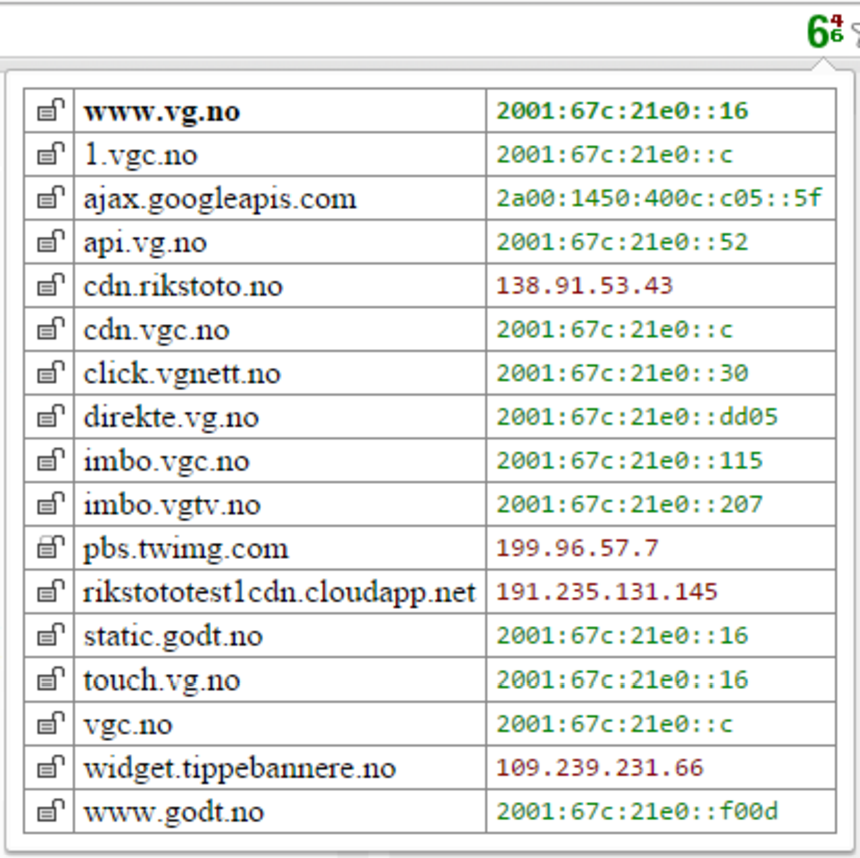
\includegraphics[scale=.4]{vg-dot-no-og-IPvFoo-i-Google-Chrome.pdf}
  \end{itemize}
\end{frame}

\section{Mozilla Firefox og IPvFox}
\begin{frame}%[allowframebreaks]
  \frametitle{Kort om IPv6}
  \framesubtitle{Mozilla Firefox og IPvFox}
  \pause
  \begin{itemize}[<+->]
  \item
    \href{https://addons.mozilla.org/en-US/firefox/addon/ipvfox/}{IPvFox}
    gjør det samme for Mozilla Firefox som IPvFoo gjør for Google
    Chrome
  \item Her er enda et eksempel fra \texttt{\url{http://vg.no/}}:\\
  \ifratio{43}{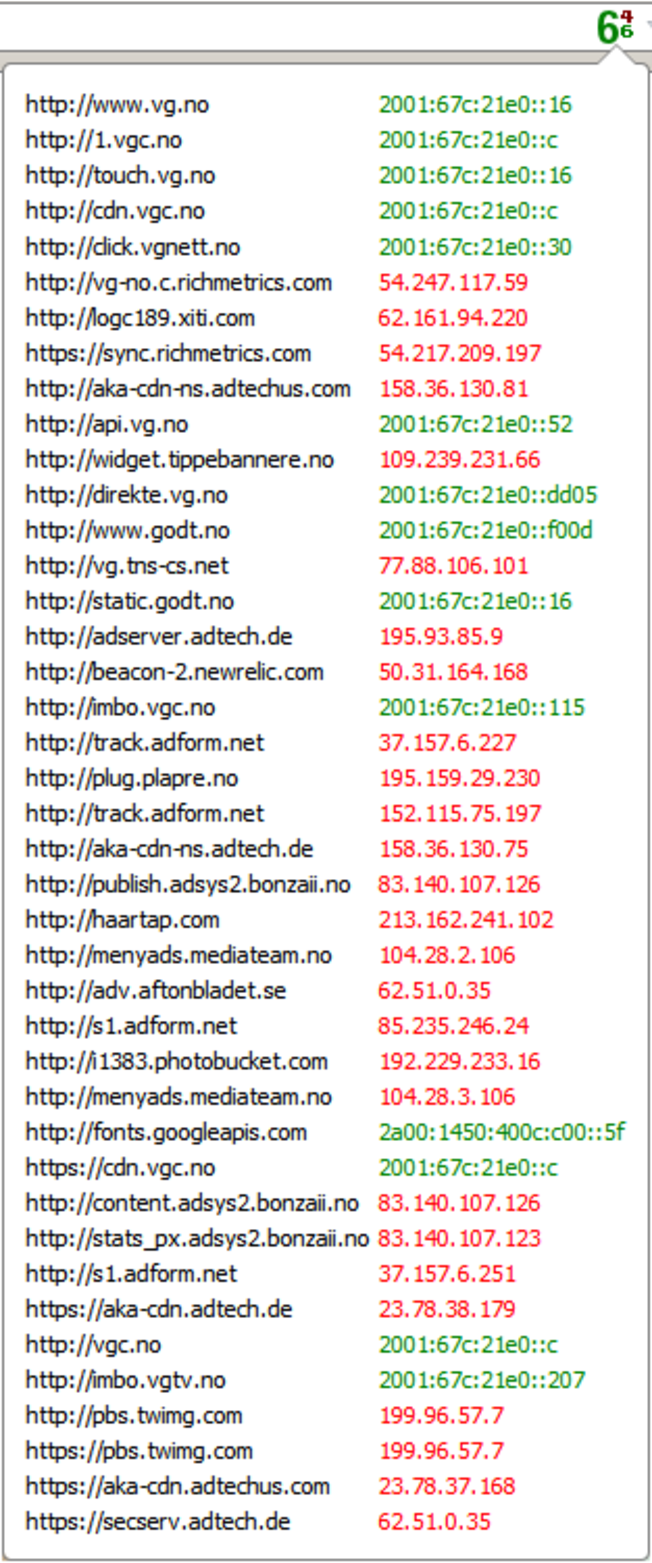
\includegraphics[scale=.8]{vg-dot-no-og-IPvFox-i-Mozilla-Firefox.pdf}}%
    {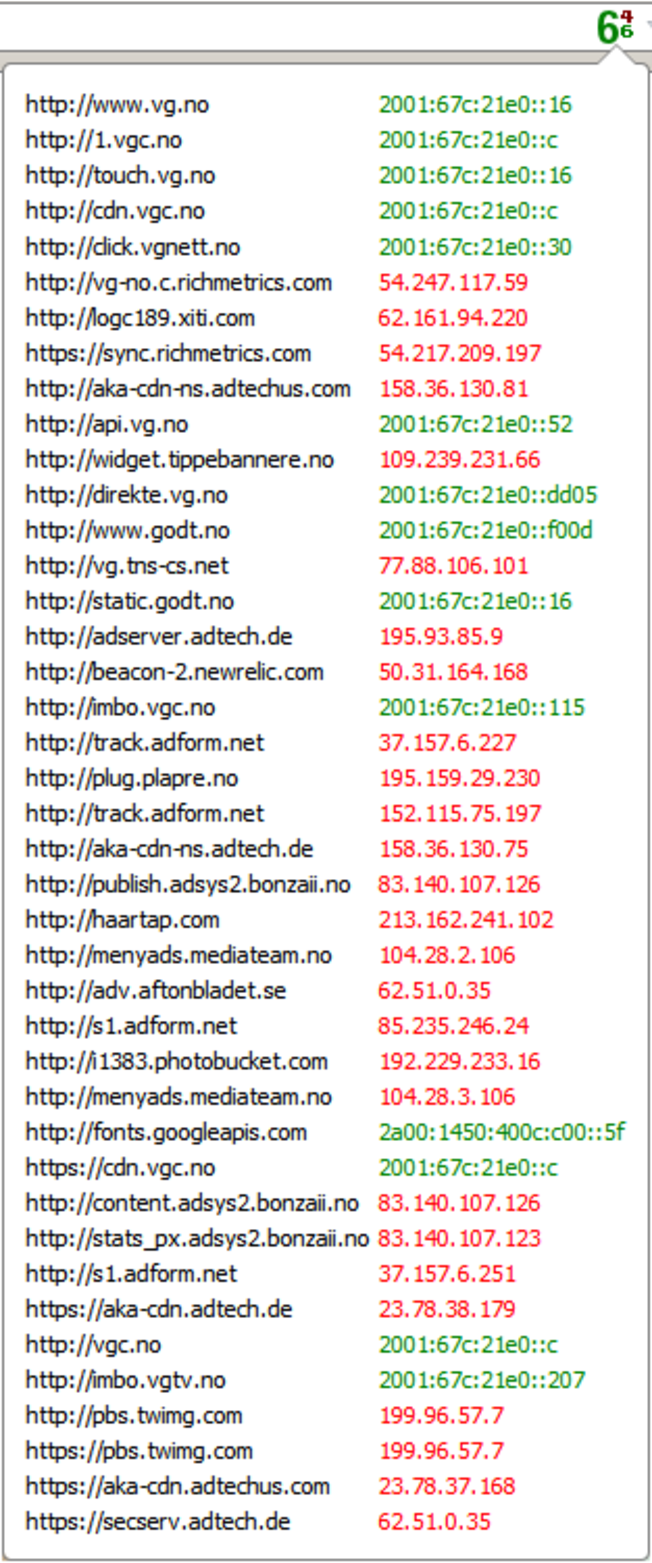
\includegraphics{vg-dot-no-og-IPvFox-i-Mozilla-Firefox.pdf}}
  \end{itemize}
\end{frame}

\part{IPv6-header}

\begin{frame}
  \partpage
\end{frame}

\section*{Oversikt over del~2: IPv6-header}
\begin{frame}[allowframebreaks]
  \frametitle{Oversikt over del~2: IPv6-header}
    \tableofcontents%[pausesections]
\end{frame}

\section{IPv6-header}
\begin{frame}%[allowframebreaks]
  \frametitle{IPv6-header}
  \pause
  \begin{center}
    \ifratio{43}{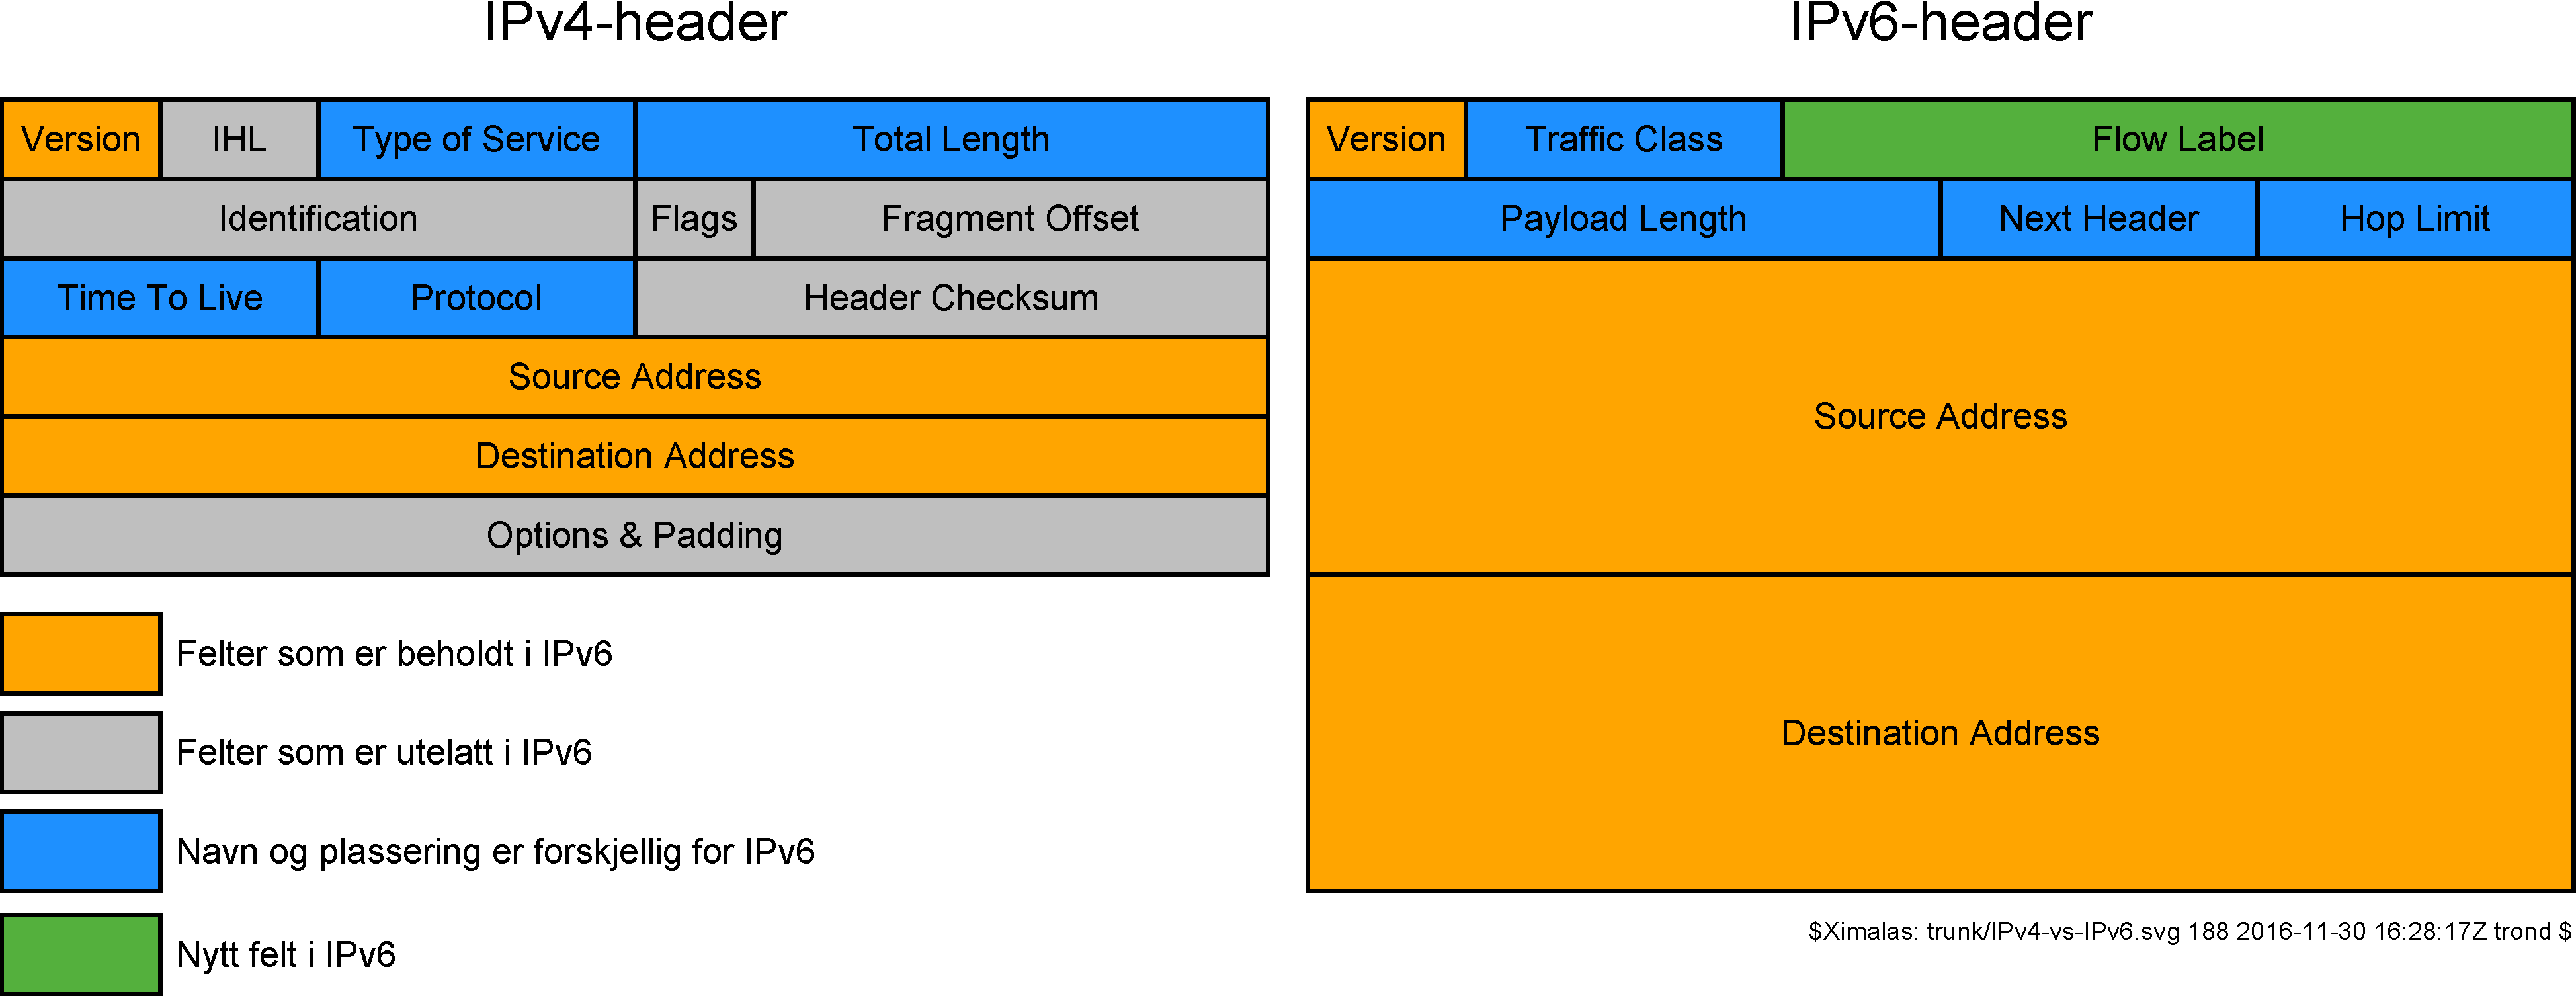
\includegraphics[scale=.18]{IPv4-vs-IPv6.pdf}}%
      {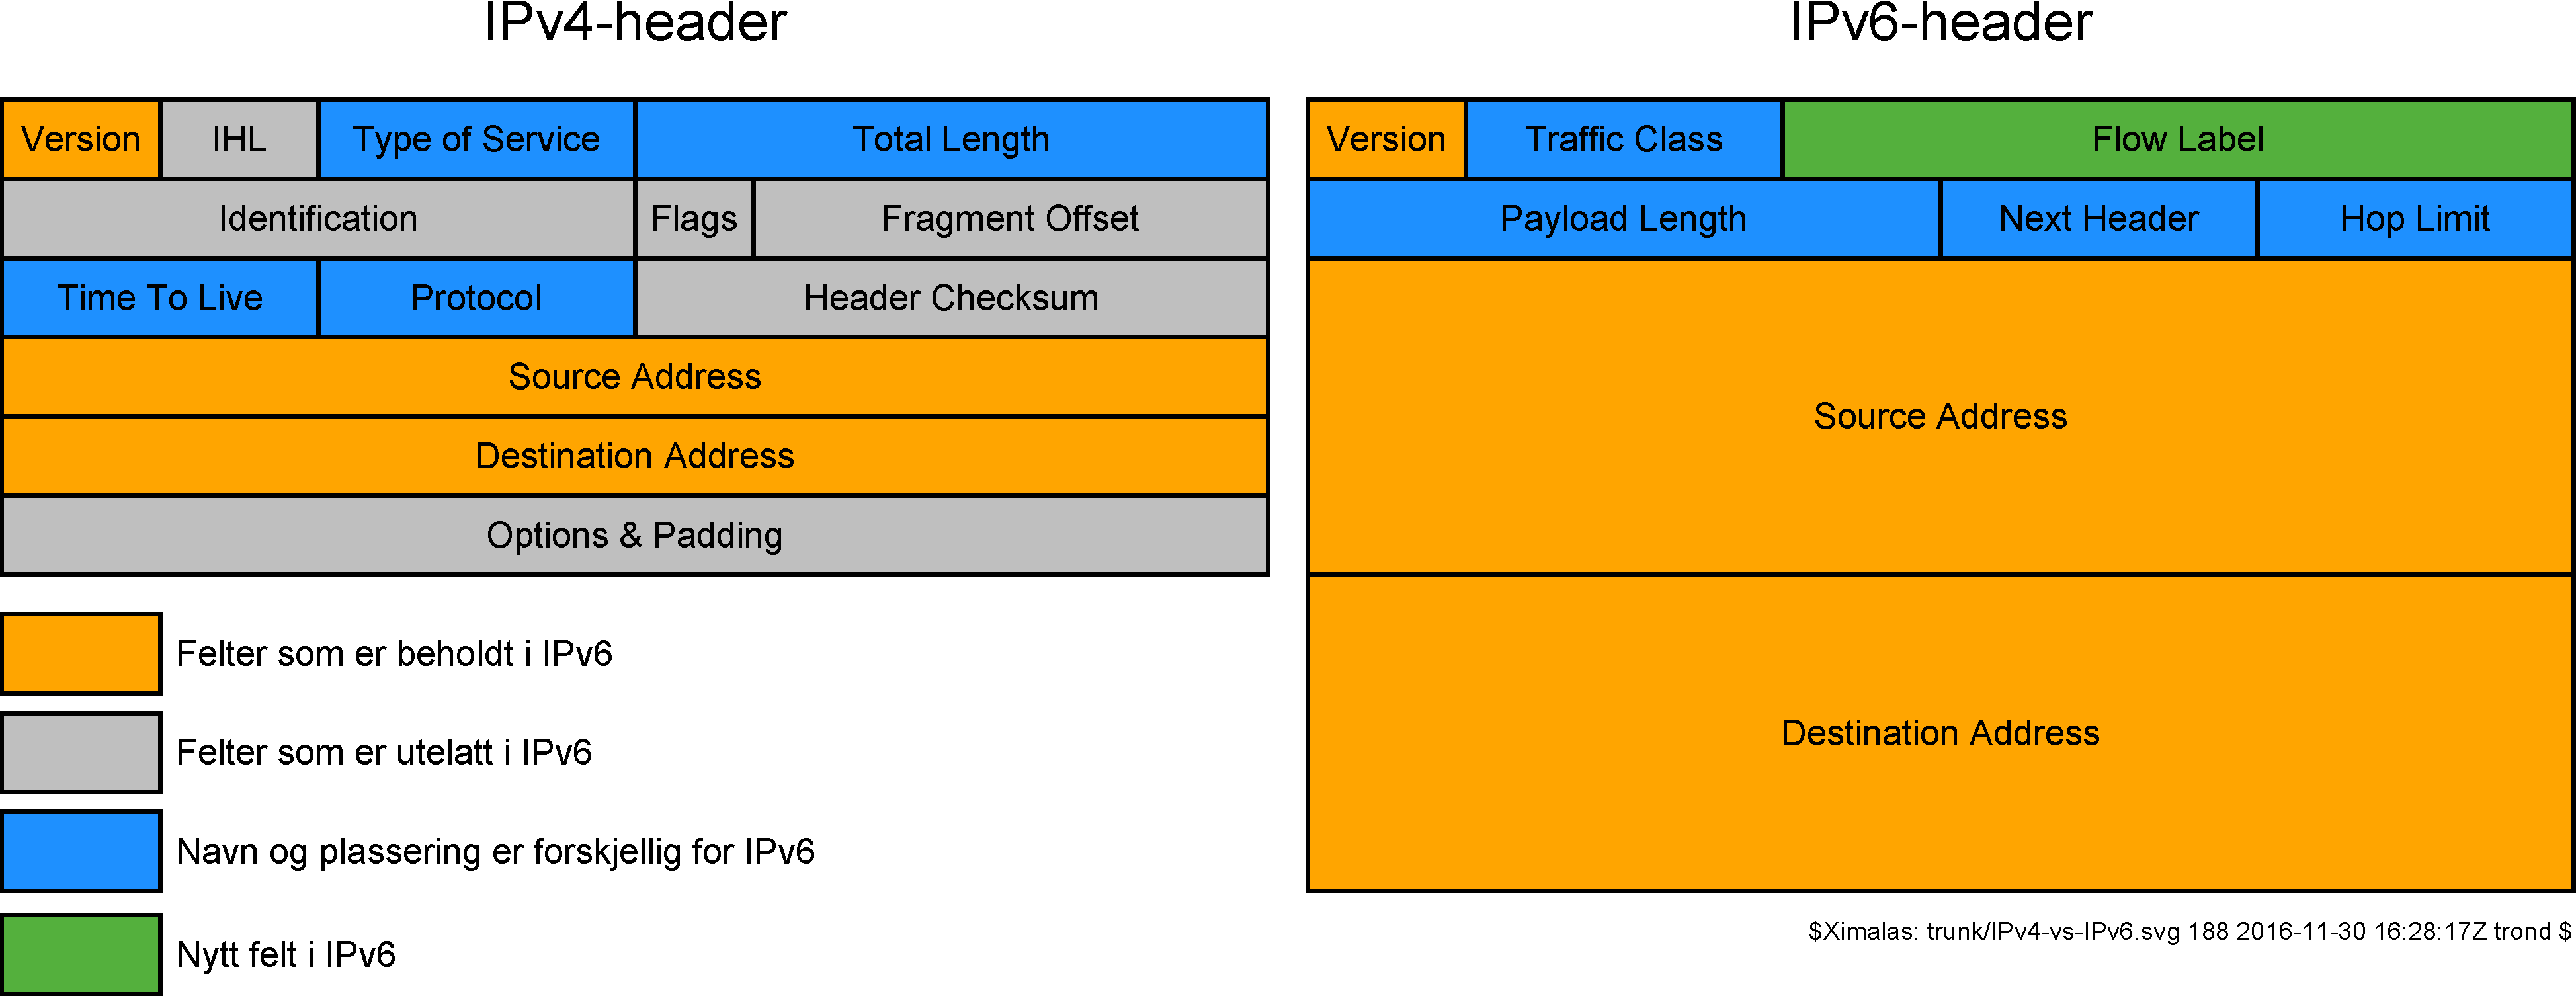
\includegraphics[scale=.2274]{IPv4-vs-IPv6.pdf}}
  \end{center}
\end{frame}

\begin{frame}%[allowframebreaks]
  \frametitle{IPv6-header}
  %\pause
  \begin{center}
    \ifratio{1610}{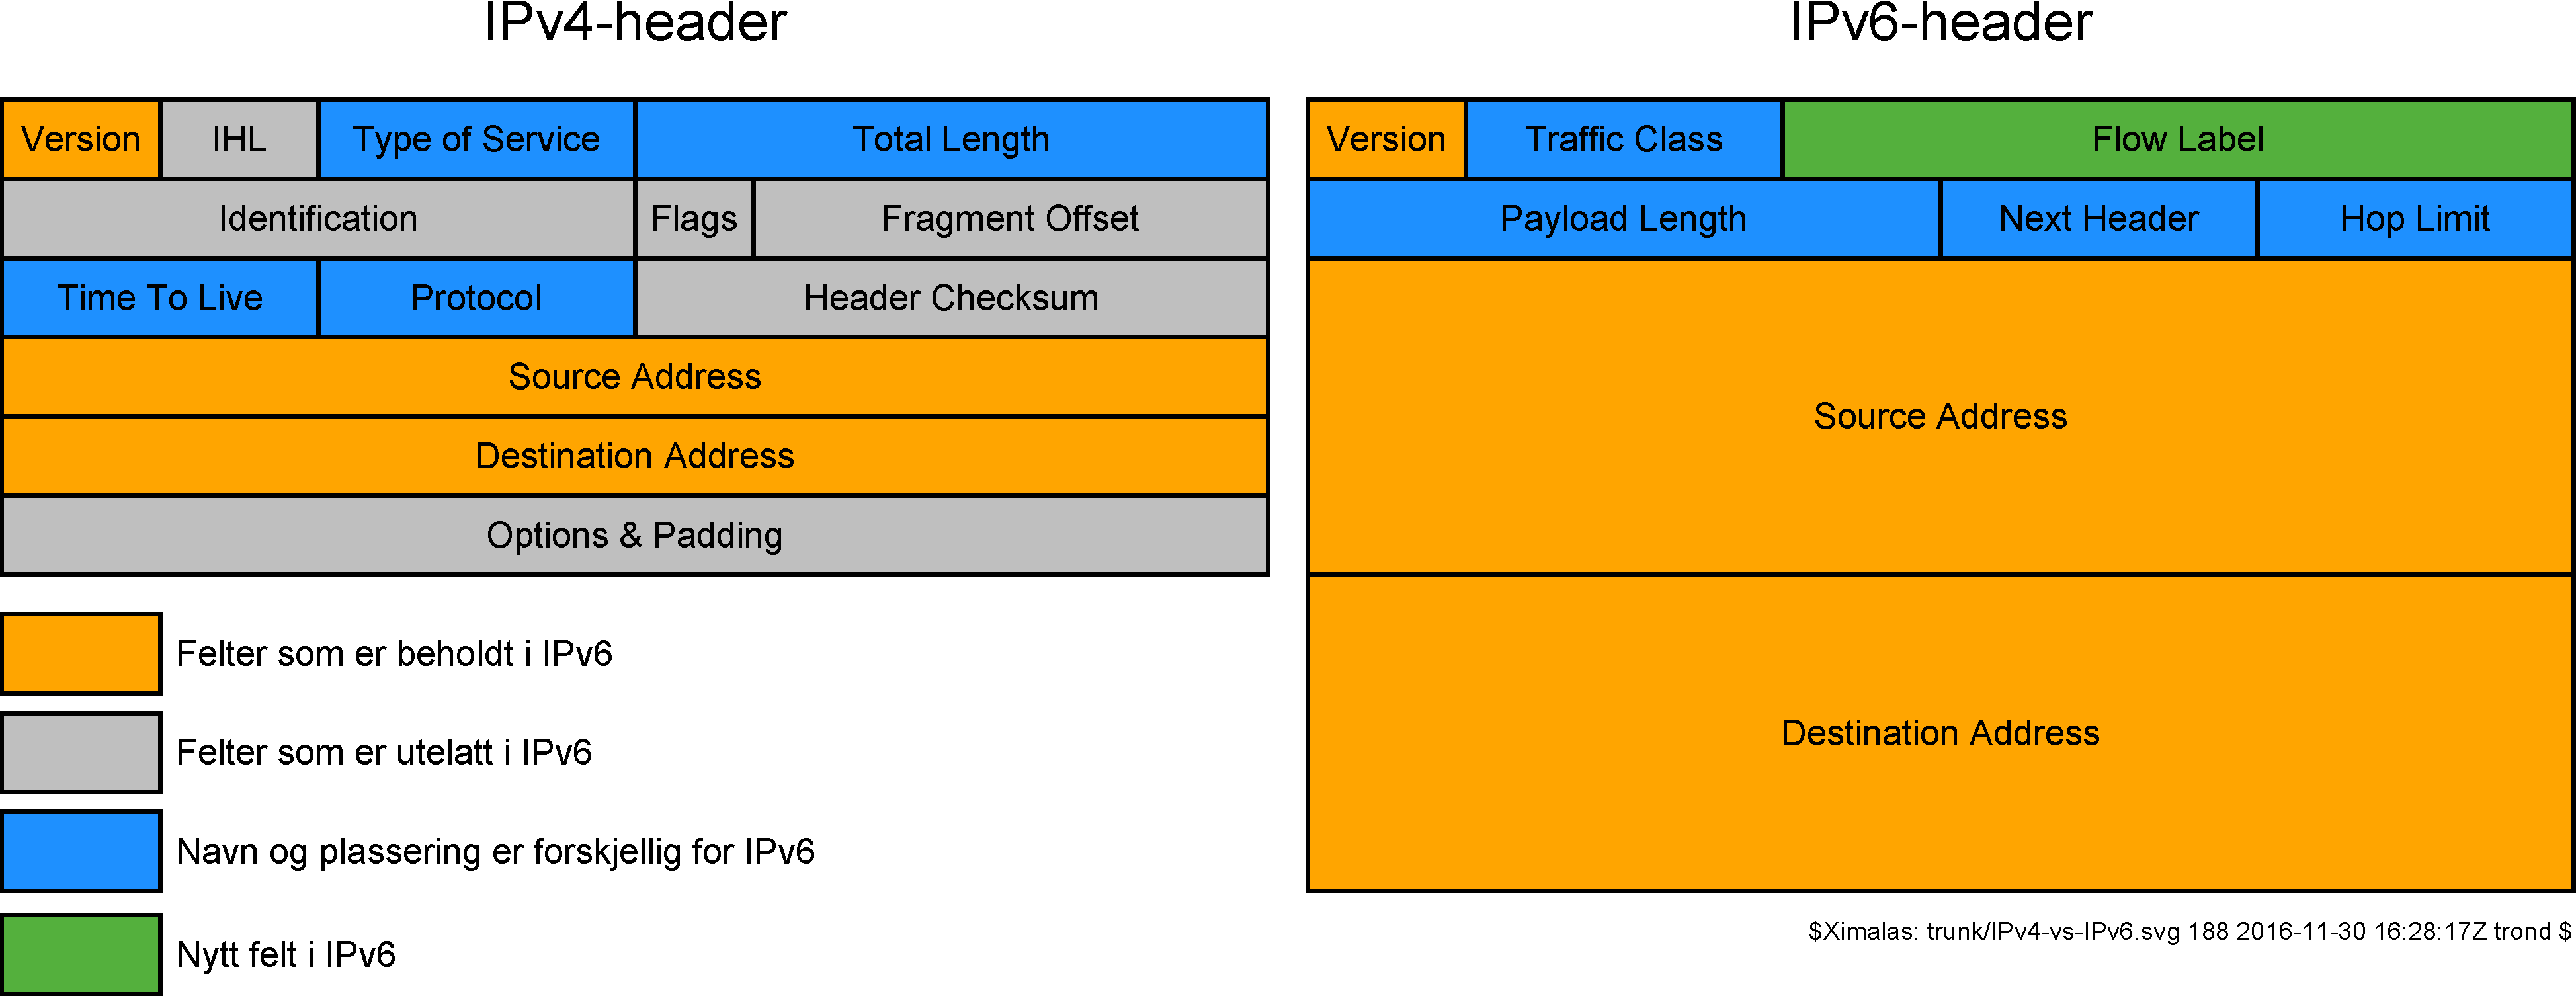
\includegraphics[scale=.190]{IPv4-vs-IPv6.pdf}}%
      {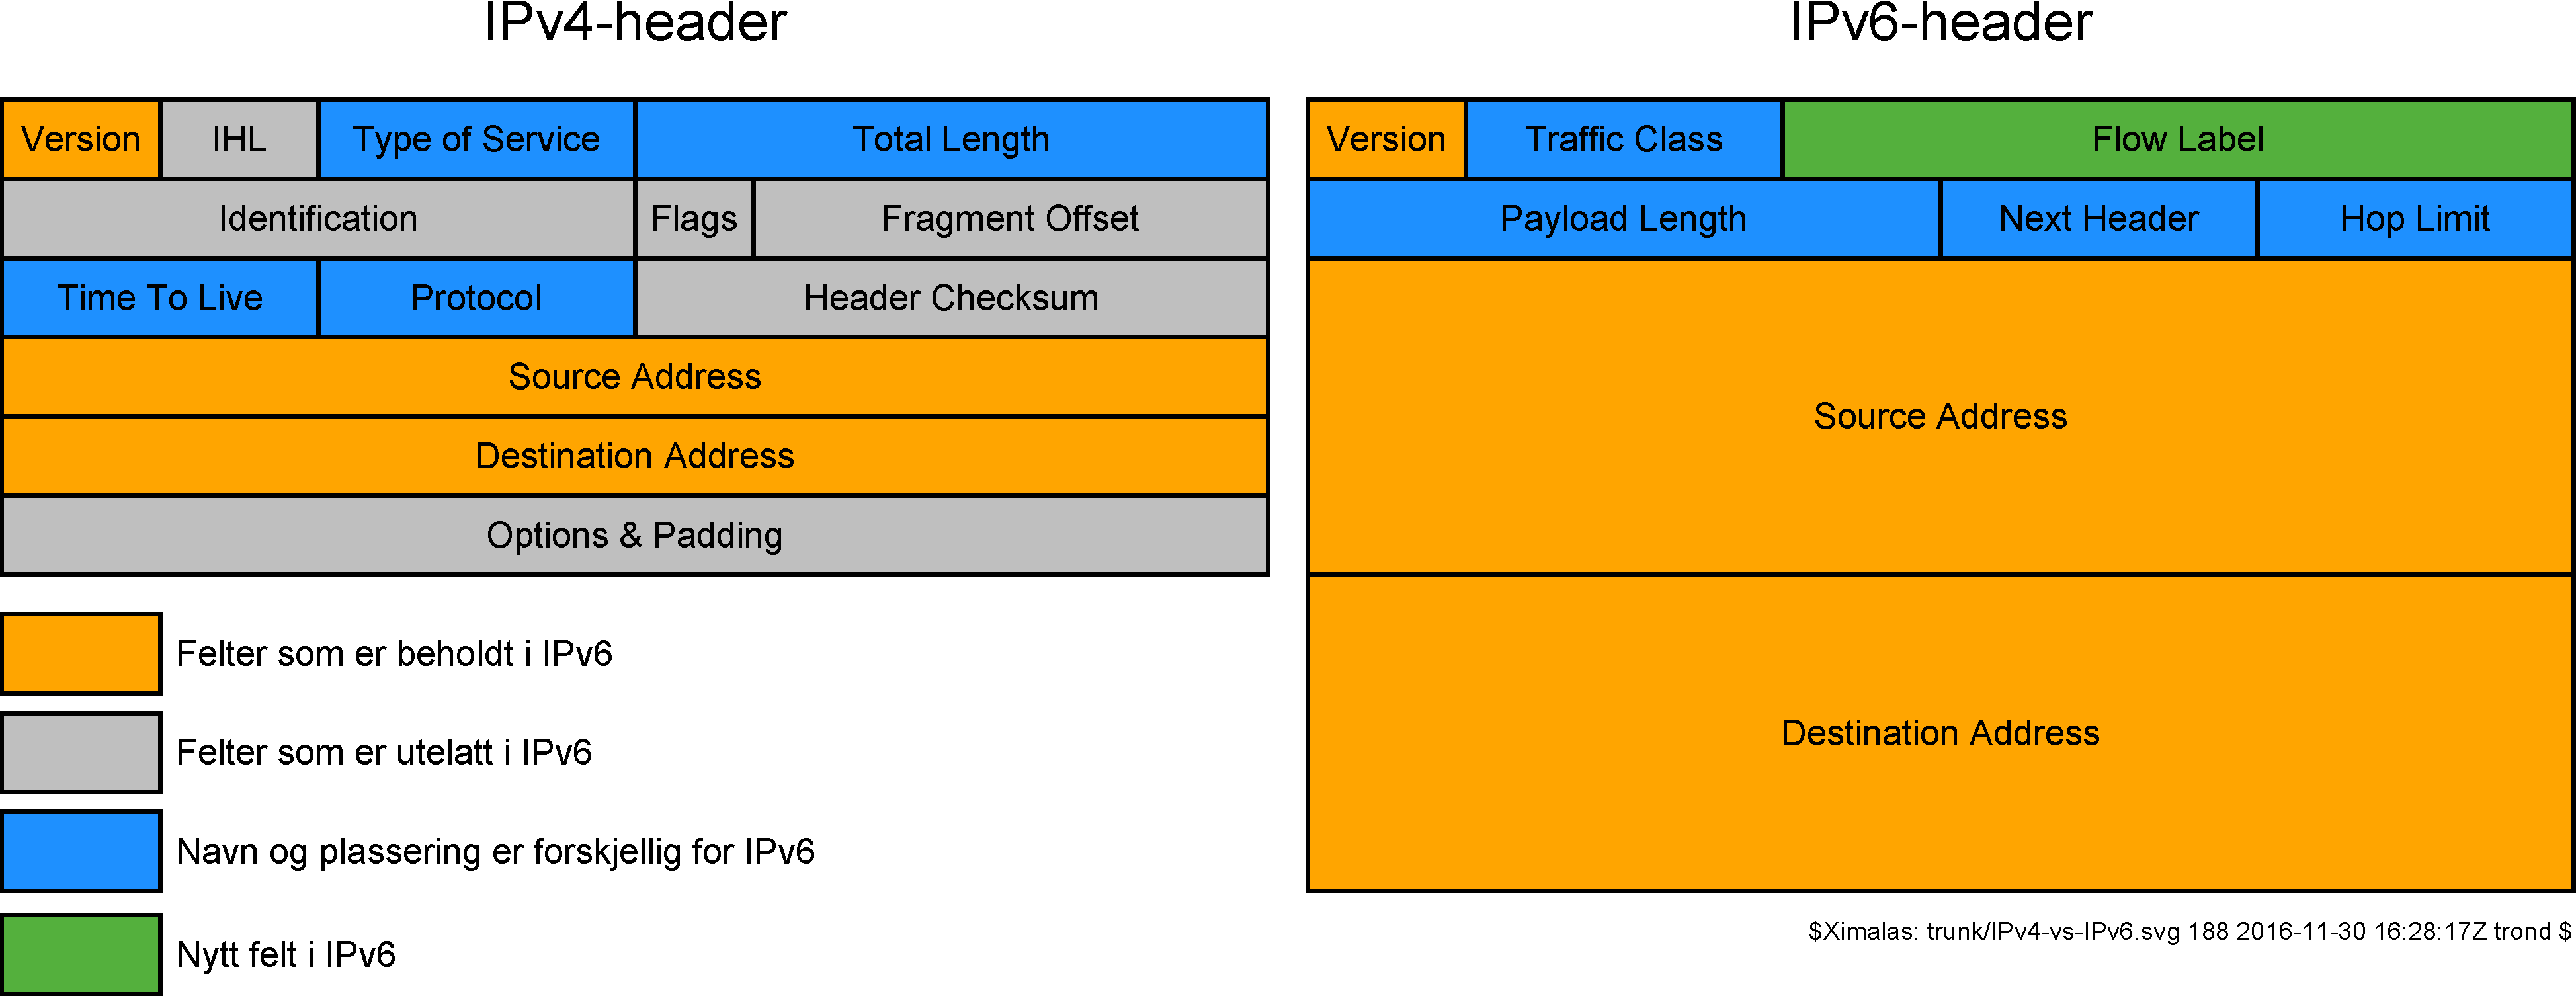
\includegraphics[scale=.17]{IPv4-vs-IPv6.pdf}}
  \end{center}

  \begin{itemize}
  \item IPv6-headeren er dobbelt så stor som IPv4-headeren
    (40/20~oktetter)
  \item IPv6-headeren har færre felter enn IPv4-headeren
  \item De utelatte feltene er i stor grad flyttet over til egne
    utvidelsesheadere
  \end{itemize}
\end{frame}

\begin{frame}%[allowframebreaks]
  \frametitle{IPv6-header}
  %\pause
  \begin{multicols}{2}
    \ifratio{43}{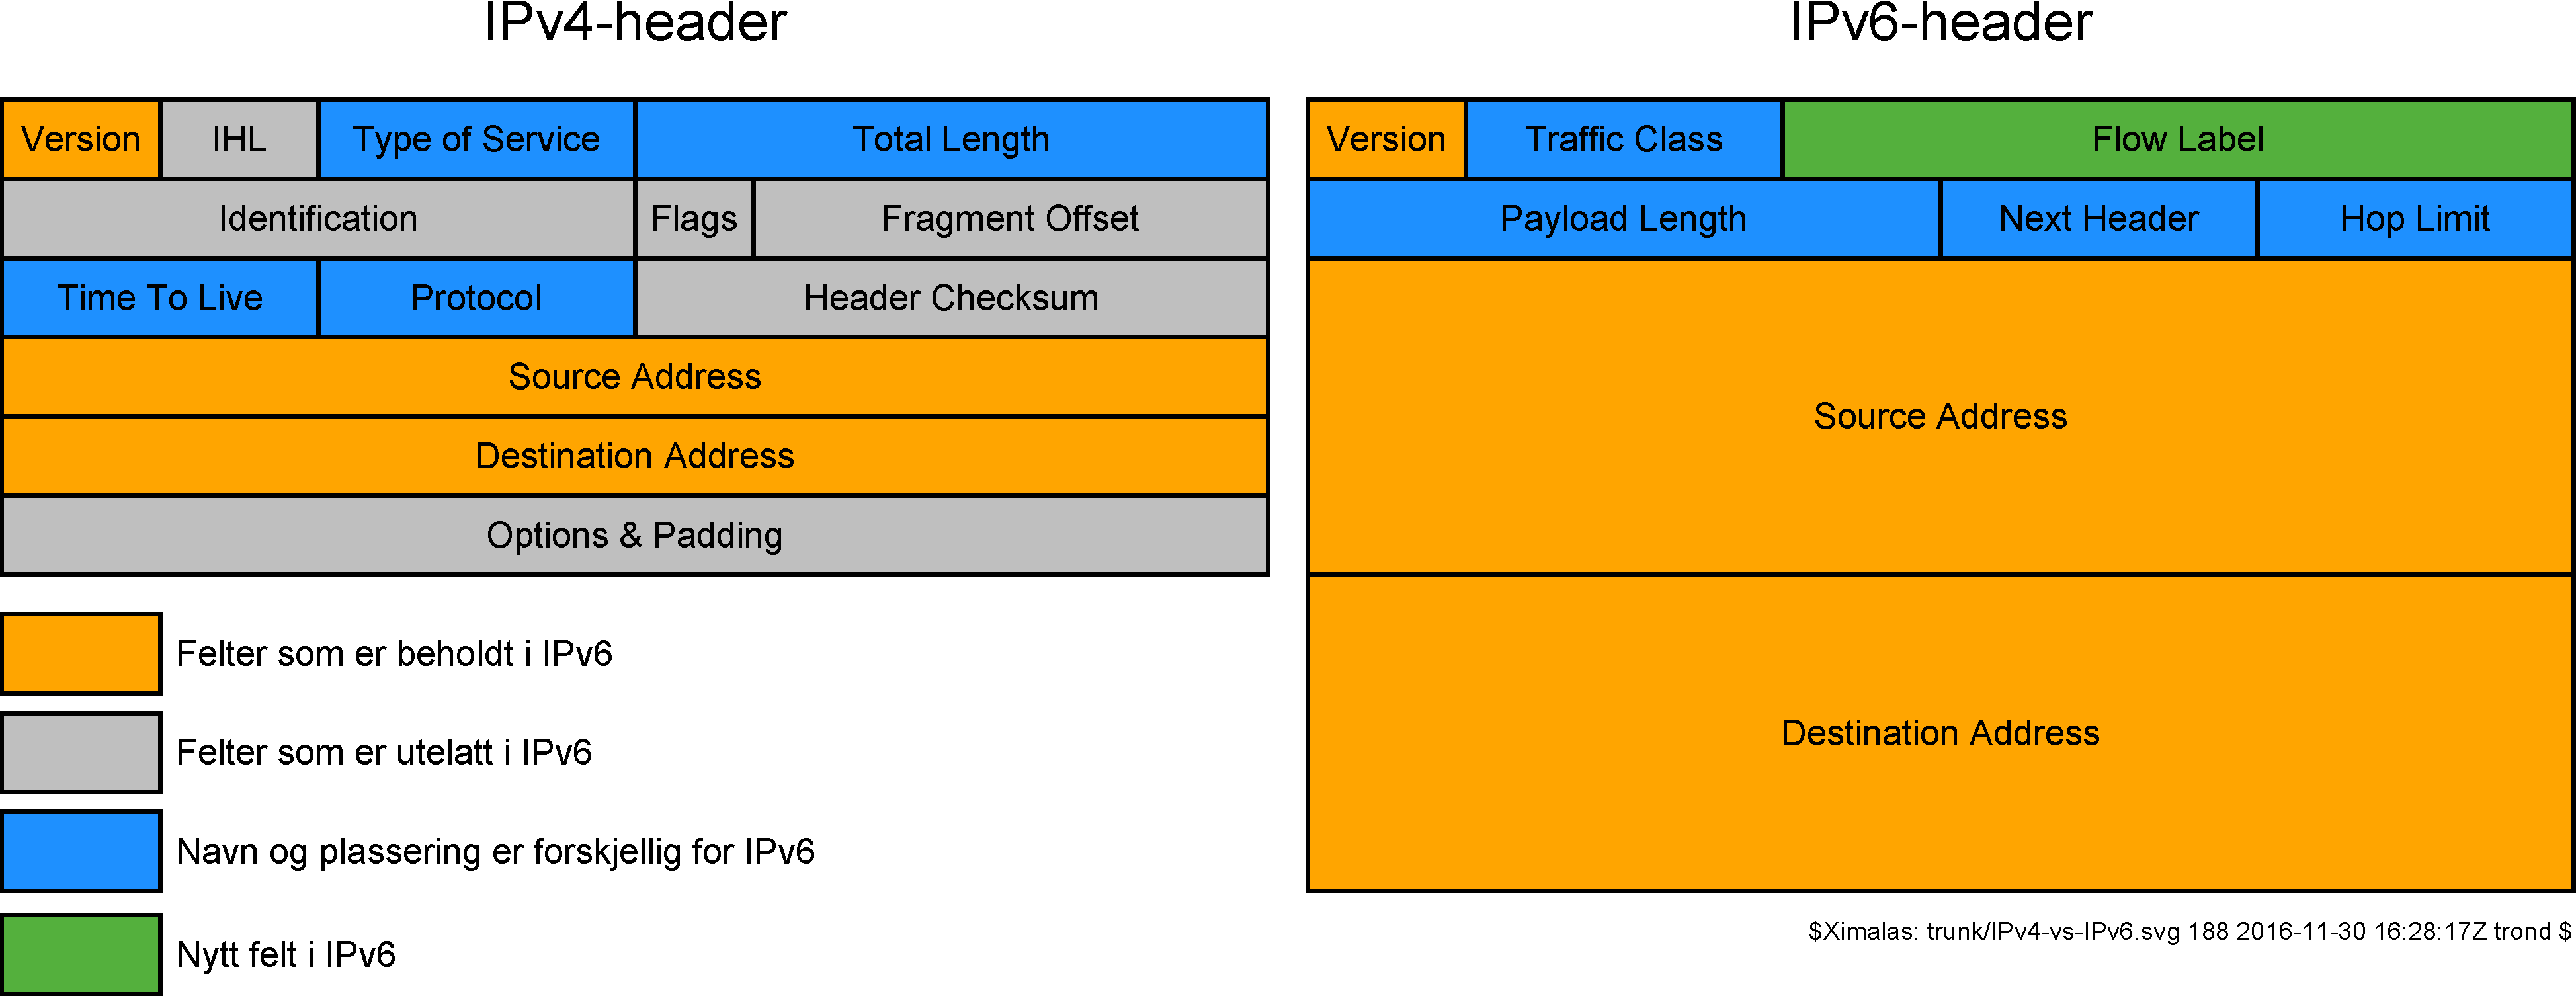
\includegraphics[scale=.0975]{IPv4-vs-IPv6.pdf}}%
      {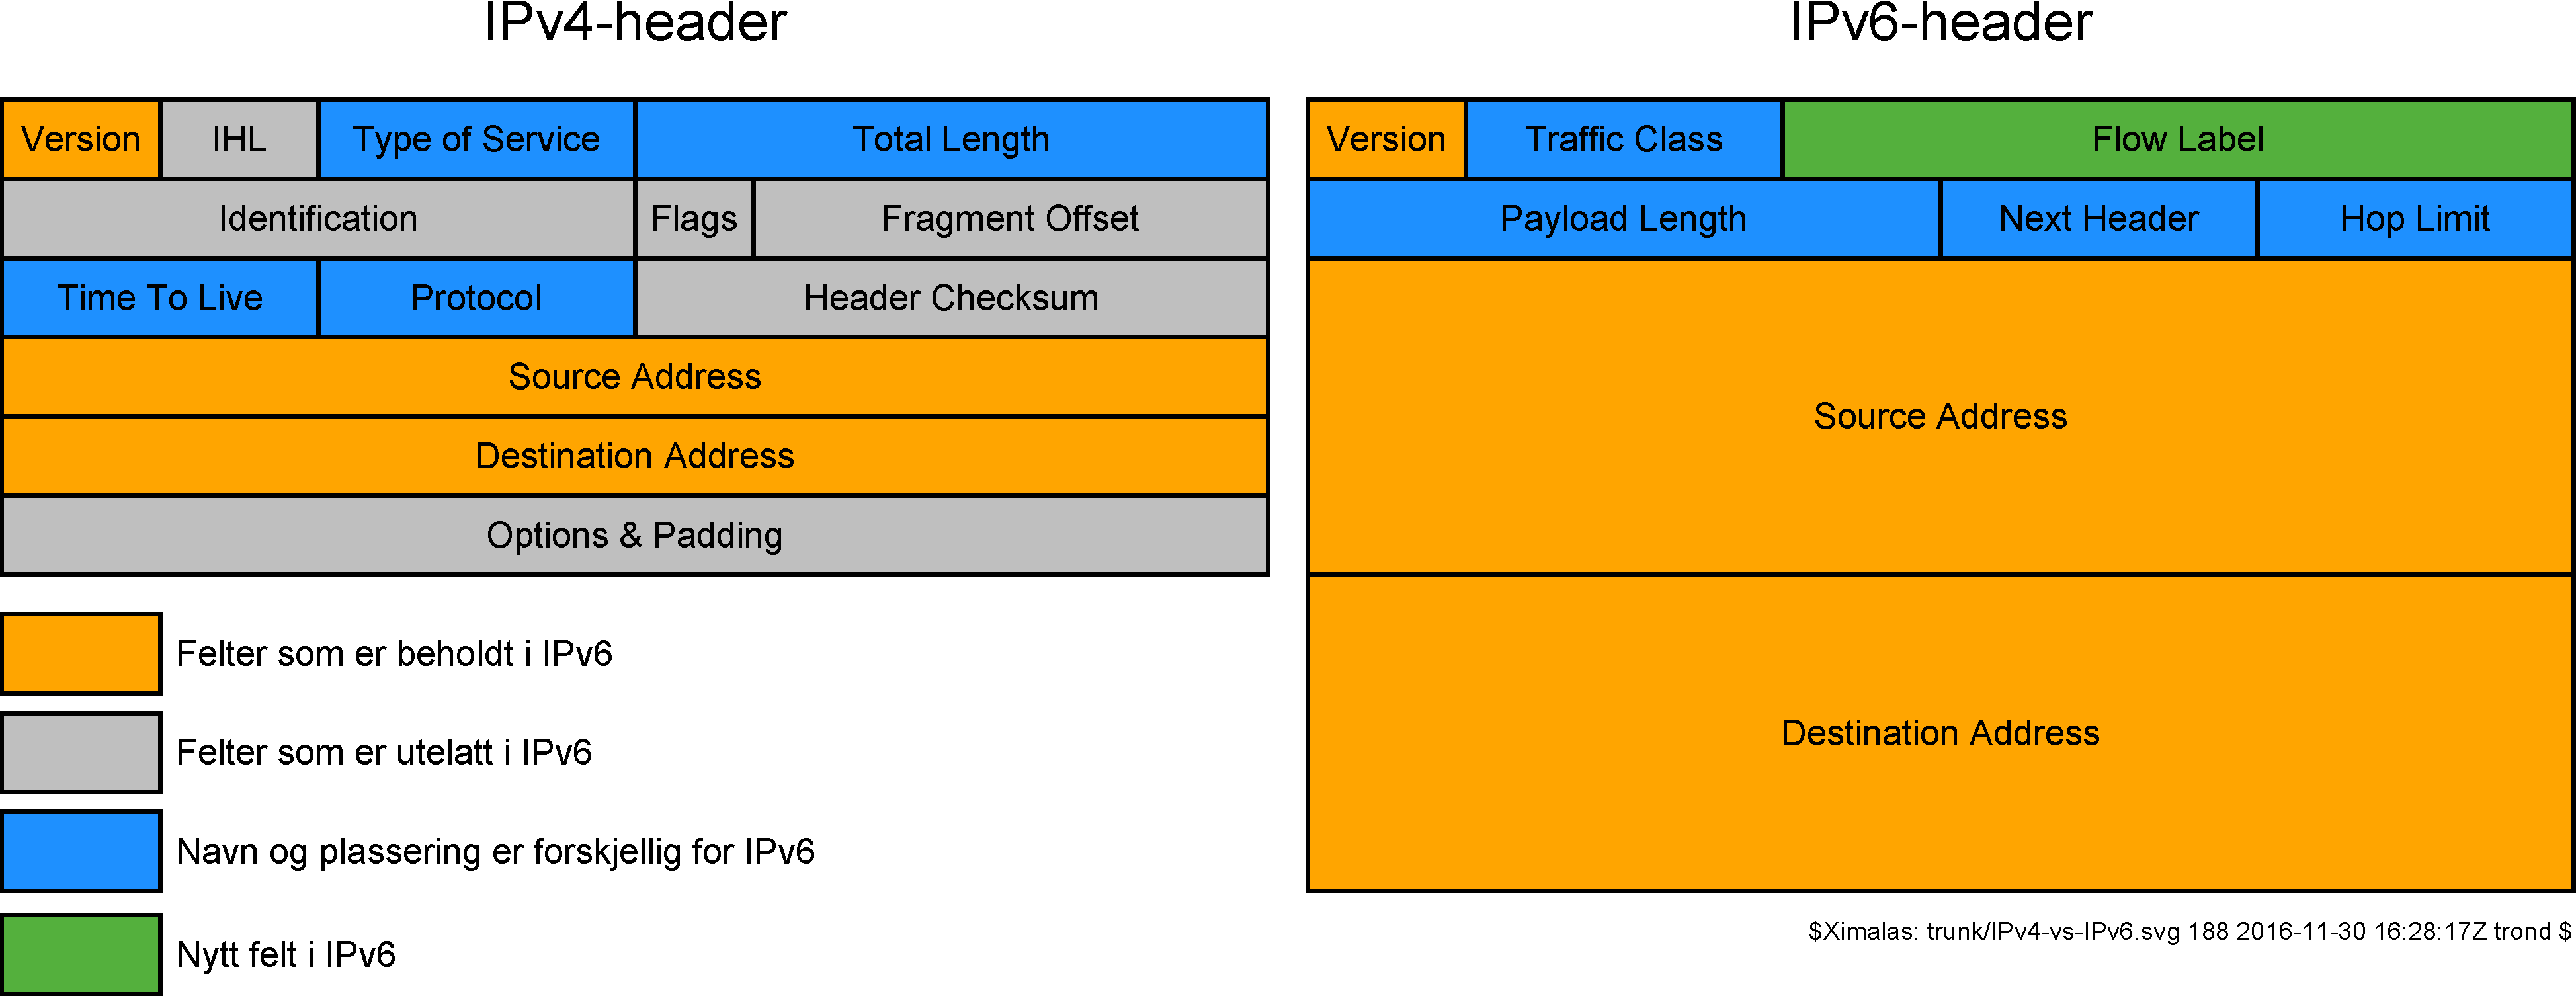
\includegraphics[scale=.1225]{IPv4-vs-IPv6.pdf}}

    \begin{itemize}[<+->]
    \item Versjonsfeltet (4 bit) settes til \texttt{0110}
    \item Traffic Class (8 bit) er det samme som Type of Service i
      IPv4
    \item Flow Label (20 bit) er et nytt felt, se neste slide
    \item Payload Length (16 bit) er det samme som Total Length i IPv4
    \item Next Header (8 bit) er det samme som Protocol i IPv4
    \item Hop Limit (8 bit) er det samme som Time To Live i IPv4
    \item Avsender og mottaker er 128-bit IPv6-adresser
    \item IPv4-feltene Internet Header Length (IHL), Identification,
      Flags, Fragment Offset, Header Checksum, Options og Padding, er
      enten fjernet for godt eller flyttet til egne utvidelsesheadere
    \end{itemize}
  \end{multicols}
\end{frame}

\subsection{Flow Label}
\begin{frame}%[allowframebreaks]
  \frametitle{IPv6-header}
  \framesubtitle{Flow Label}
  \pause
  \begin{itemize}[<+->]
  \item Flow Label-feltet kan brukes av sanntidsapplikasjoner
  \item Flow Label-verdien angir pakker som tilhører samme sesjon
  \item Routere bør videresende pakker med samme verdi i Flow
    Label-feltet fra samme avsender på samme grensesnitt, slik at
    rekkefølgen bevares
  \item Verdien 0 (null) brukes for individuelle pakker
  \item Routere bør videresende pakker med 0 i Flow Label-feltet fra
    samme avsender på samme grensesnitt, slik at rekkefølgen bevares
  \item Tilfeldig valgte verdier brukes for pakker som hører sammen
  \item Flow Label-feltet kan også brukes til å smugle data sammen med
    legitim trafikk, eller merke slik trafikk, se avsnitt 6.1 i
    \rfc{6437}
  \item Se \rfc{2460}, \rfc{3595}, \rfc{6294}, \rfc{6436} og \rfc{6437}
  \end{itemize}
\end{frame}

\section{Utvidelsesheadere}
\begin{frame}%[allowframebreaks]
  \frametitle{Utvidelsesheadere}
  \pause
  \begin{itemize}[<+->]
  \item Utvidelsesheaderne finnes i stort antall:
    \begin{enumerate}[<+->]
    \item Hop-by-hop Options Header
    \item Destination Options Header
    \item Routing Header
    \item Fragment Header
    \item Authentication Header
    \item Encapsulating Security Payload
    \item Mobility Header
    \end{enumerate}
  \item Se \rfc{2460}, \rfc{4302}, \rfc{4303}, \rfc{6275} og
    \rfc{7045}
  \end{itemize}
\end{frame}

\subsection{Hop-by-hop Options Header}
\begin{frame}[fragile]%[allowframebreaks]
  \frametitle{Utvidelsesheadere}
  \framesubtitle{Hop-by-hop Options Header}
  \pause
\begin{Verbatim}[fontsize=\tiny]
+-+-+-+-+-+-+-+-+-+-+-+-+-+-+-+-+-+-+-+-+-+-+-+-+-+-+-+-+-+-+-+-+
|  Next Header  |  Hdr Ext Len  |                               |
+-+-+-+-+-+-+-+-+-+-+-+-+-+-+-+-+                               +
|                                                               |
.                                                               .
.                            Options                            .
.                                                               .
|                                                               |
+-+-+-+-+-+-+-+-+-+-+-+-+-+-+-+-+-+-+-+-+-+-+-+-+-+-+-+-+-+-+-+-+
\end{Verbatim}

  \pause
  \begin{itemize}[<+->]
  \item Protokollnummer: 0
  \item Hop-by-hop Options Header må komme før andre Options Headere
    og før payload
  \item Alle ledd bør undersøke Hop-by-hop Options Header og dens innhold
  \item Høyhastighetsroutere vil enten ignorere H-b-H eller la en
    saktegående routingprosess ta seg av slike pakker
  \end{itemize}
\end{frame}

\begin{frame}[fragile]%[allowframebreaks]
  \frametitle{Utvidelsesheadere}
  \framesubtitle{Hop-by-hop Options Header}
  %\pause
  \begin{itemize}[<+->]
  \item Valgene \texttt{Pad1} og \texttt{PadN} er definert i
    \rfc{2460}
  \item Andre valg: Jumbo Payload \prfc{2675}, RPL Option \prfc{6553},
    Tunnel Encapsulation Limit \prfc{2473}, Router Alert \prfc{2711},
    Quick-Start \prfc{4782}, CALIPSO \prfc{5570}, SMF\_DPD
    \prfc{6621}, Home Address \prfc{6275}, ILNP nonce \prfc{6744},
    Line-Identification Option \prfc{6788}, IP\_DFF \prfc{6971}
  \item Ref.:
    \texttt{\url{http://www.iana.org/assignments/ipv6-parameters/ipv6-parameters.xhtml}}
  \end{itemize}
\end{frame}

\subsection{Destination Options Header}
\begin{frame}[fragile]%[allowframebreaks]
  \frametitle{Utvidelsesheadere}
  \framesubtitle{Destination Options Header}
  \pause
\begin{Verbatim}[fontsize=\tiny]
+-+-+-+-+-+-+-+-+-+-+-+-+-+-+-+-+-+-+-+-+-+-+-+-+-+-+-+-+-+-+-+-+
|  Next Header  |  Hdr Ext Len  |                               |
+-+-+-+-+-+-+-+-+-+-+-+-+-+-+-+-+                               +
|                                                               |
.                                                               .
.                            Options                            .
.                                                               .
|                                                               |
+-+-+-+-+-+-+-+-+-+-+-+-+-+-+-+-+-+-+-+-+-+-+-+-+-+-+-+-+-+-+-+-+
\end{Verbatim}

  \pause
  \begin{itemize}[<+->]
  \item Protokollnummer: 60
  \end{itemize}
\end{frame}

\subsection{Routing Header}
\begin{frame}[fragile]%[allowframebreaks]
  \frametitle{Utvidelsesheadere}
  \framesubtitle{Routing Header}
  \pause
\begin{Verbatim}[fontsize=\tiny]
+-+-+-+-+-+-+-+-+-+-+-+-+-+-+-+-+-+-+-+-+-+-+-+-+-+-+-+-+-+-+-+-+
|  Next Header  |  Hdr Ext Len  |  Routing Type | Segments Left |
+-+-+-+-+-+-+-+-+-+-+-+-+-+-+-+-+-+-+-+-+-+-+-+-+-+-+-+-+-+-+-+-+
|                                                               |
.                                                               .
.                       type-specific data                      .
.                                                               .
|                                                               |
+-+-+-+-+-+-+-+-+-+-+-+-+-+-+-+-+-+-+-+-+-+-+-+-+-+-+-+-+-+-+-+-+
\end{Verbatim}

  \pause
  \begin{itemize}[<+->]
  \item Protokollnummer: 43
  \end{itemize}
\end{frame}

\subsection{Fragment Header}
\begin{frame}[fragile]%[allowframebreaks]
  \frametitle{Utvidelsesheadere}
  \framesubtitle{Fragment Header}
  \pause
\begin{Verbatim}[fontsize=\tiny]
+-+-+-+-+-+-+-+-+-+-+-+-+-+-+-+-+-+-+-+-+-+-+-+-+-+-+-+-+-+-+-+-+
|  Next Header  |   Reserved    |      Fragment Offset    |Res|M|
+-+-+-+-+-+-+-+-+-+-+-+-+-+-+-+-+-+-+-+-+-+-+-+-+-+-+-+-+-+-+-+-+
|                         Identification                        |
+-+-+-+-+-+-+-+-+-+-+-+-+-+-+-+-+-+-+-+-+-+-+-+-+-+-+-+-+-+-+-+-+
\end{Verbatim}

  \pause
  \begin{itemize}[<+->]
  \item Protokollnummer: 44
  \end{itemize}
\end{frame}

\subsection{Authentication Header}
\begin{frame}[fragile]%[allowframebreaks]
  \frametitle{Utvidelsesheadere}
  \framesubtitle{Authentication Header}
  \pause
\begin{Verbatim}[fontsize=\tiny]
 0                   1                   2                   3
 0 1 2 3 4 5 6 7 8 9 0 1 2 3 4 5 6 7 8 9 0 1 2 3 4 5 6 7 8 9 0 1
+-+-+-+-+-+-+-+-+-+-+-+-+-+-+-+-+-+-+-+-+-+-+-+-+-+-+-+-+-+-+-+-+
| Next Header   |  Payload Len  |          RESERVED             |
+-+-+-+-+-+-+-+-+-+-+-+-+-+-+-+-+-+-+-+-+-+-+-+-+-+-+-+-+-+-+-+-+
|                 Security Parameters Index (SPI)               |
+-+-+-+-+-+-+-+-+-+-+-+-+-+-+-+-+-+-+-+-+-+-+-+-+-+-+-+-+-+-+-+-+
|                    Sequence Number Field                      |
+-+-+-+-+-+-+-+-+-+-+-+-+-+-+-+-+-+-+-+-+-+-+-+-+-+-+-+-+-+-+-+-+
|                                                               |
+                Integrity Check Value-ICV (variable)           |
|                                                               |
+-+-+-+-+-+-+-+-+-+-+-+-+-+-+-+-+-+-+-+-+-+-+-+-+-+-+-+-+-+-+-+-+
\end{Verbatim}

  \pause
  \begin{itemize}[<+->]
  \item Protokollnummer: 51
  \end{itemize}
\end{frame}

\subsection{Encapsulating Security Payload}
\begin{frame}[fragile]%[allowframebreaks]
  \frametitle{Utvidelsesheadere}
  \framesubtitle{Encapsulating Security Payload}
  \pause
\begin{Verbatim}[fontsize=\tiny]
 0                   1                   2                   3
 0 1 2 3 4 5 6 7 8 9 0 1 2 3 4 5 6 7 8 9 0 1 2 3 4 5 6 7 8 9 0 1
+-+-+-+-+-+-+-+-+-+-+-+-+-+-+-+-+-+-+-+-+-+-+-+-+-+-+-+-+-+-+-+-+
|               Security Parameters Index (SPI)                 |
+-+-+-+-+-+-+-+-+-+-+-+-+-+-+-+-+-+-+-+-+-+-+-+-+-+-+-+-+-+-+-+-+
|                      Sequence Number                          |
+-+-+-+-+-+-+-+-+-+-+-+-+-+-+-+-+-+-+-+-+-+-+-+-+-+-+-+-+-+-+-+-+
|                    Payload Data* (variable)                   |
~                                                               ~
|                                                               |
+               +-+-+-+-+-+-+-+-+-+-+-+-+-+-+-+-+-+-+-+-+-+-+-+-+
|               |     Padding (0-255 bytes)                     |
+-+-+-+-+-+-+-+-+               +-+-+-+-+-+-+-+-+-+-+-+-+-+-+-+-+
|                               |  Pad Length   | Next Header   |
+-+-+-+-+-+-+-+-+-+-+-+-+-+-+-+-+-+-+-+-+-+-+-+-+-+-+-+-+-+-+-+-+
|         Integrity Check Value-ICV   (variable)                |
~                                                               ~
|                                                               |
+-+-+-+-+-+-+-+-+-+-+-+-+-+-+-+-+-+-+-+-+-+-+-+-+-+-+-+-+-+-+-+-+
\end{Verbatim}

  \pause
  \begin{itemize}[<+->]
  \item Protokollnummer: 50
  \end{itemize}
\end{frame}

\subsection{Mobility Header}
\begin{frame}[fragile]%[allowframebreaks]
  \frametitle{Utvidelsesheadere}
  \framesubtitle{Mobility Header}
  \pause
\begin{Verbatim}[fontsize=\tiny]
+-+-+-+-+-+-+-+-+-+-+-+-+-+-+-+-+-+-+-+-+-+-+-+-+-+-+-+-+-+-+-+-+
| Payload Proto |  Header Len   |   MH Type     |   Reserved    |
+-+-+-+-+-+-+-+-+-+-+-+-+-+-+-+-+-+-+-+-+-+-+-+-+-+-+-+-+-+-+-+-+
|           Checksum            |                               |
+-+-+-+-+-+-+-+-+-+-+-+-+-+-+-+-+                               |
|                                                               |
.                                                               .
.                       Message Data                            .
.                                                               .
|                                                               |
+-+-+-+-+-+-+-+-+-+-+-+-+-+-+-+-+-+-+-+-+-+-+-+-+-+-+-+-+-+-+-+-+
\end{Verbatim}

  \pause
  \begin{itemize}[<+->]
  \item Protokollnummer: 135
  \end{itemize}
\end{frame}

\part{IPv6 over Ethernet}

\begin{frame}
  \partpage
\end{frame}

\section*{Oversikt over del~3: IPv6 over Ethernet}
\begin{frame}[allowframebreaks]
  \frametitle{Oversikt over del~3: IPv6 over Ethernet}
    \tableofcontents%[pausesections]
\end{frame}

\section{IPv6 over Ethernet}
\begin{frame}%[allowframebreaks]
  \frametitle{IPv6 over Ethernet}
  \pause
  \begin{itemize}[<+->]
  \item \rfc{2464} definerer frameformatet for IPv6-datagrammer over
    Ethernet
  \item IPv6-datagrammer fraktes i standard Ethernetformat, \rfc{894}
    \begin{itemize}[<+->]
    \item Først angis mottakerens MAC-48-adresse
    \item Deretter angis avsenders MAC-48-adresse
    \item Frametypen settes til \texttt{86DD} (heksadesimalt)
    \item Deretter følger IPv6-header og resten av datagrammet
    \end{itemize}
  \item Standard MTU for IPv6 over Ethernet er 1500 oktetter
  \item Minste tillatte MTU for IPv6 er 1280 oktetter
  \item Er største tilgjengelige MTU mindre enn 1280 oktetter, så må
    lagene under IPv6 sørge for fragmentering og sammensetting av
    IPv6-datagrammene \prfc{2460}
  \end{itemize}
\end{frame}

\begin{frame}[fragile]%[allowframebreaks]
  \frametitle{IPv6 over Ethernet}
  \pause
  \noindent
  Programmet \href{http://www.wireshark.org/}{Wireshark} fremstilte
  følgende lag-2-informasjon om en utsendt IPv6-pakke:

\begin{Verbatim}[fontsize=\tiny]
Ethernet II, Src: AsustekC_f2:72:40 (00:26:18:f2:72:40), Dst: Cisco_77:14:57 (00:17:e0:77:14:57)
    Destination: Cisco_77:14:57 (00:17:e0:77:14:57)
        Address: Cisco_77:14:57 (00:17:e0:77:14:57)
        .... ..0. .... .... .... .... = LG bit: Globally unique address (factory default)
        .... ...0 .... .... .... .... = IG bit: Individual address (unicast)
    Source: AsustekC_f2:72:40 (00:26:18:f2:72:40)
        Address: AsustekC_f2:72:40 (00:26:18:f2:72:40)
        .... ..0. .... .... .... .... = LG bit: Globally unique address (factory default)
        .... ...0 .... .... .... .... = IG bit: Individual address (unicast)
    Type: IPv6 (0x86dd)
\end{Verbatim}

  \pause
  \begin{itemize}[<+->]
  \item Presentert som heksadesimale oktetter/byter:
  \item \texttt{\color{red}00 17 E0 77 14 57 \color{violet}00 26 18 F2 72 40 \color{black}86 DD}
    \begin{itemize}[<+->]
    \item \texttt{\color{red}00 17 E0 77 14 57} er MAC-48-adressa til mottakeren, routeren
    \item \texttt{\color{violet}00 26 18 F2 72 40} er MAC-48-adressa til avsenderen, klienten
    \item \texttt{86 DD} angir at et IPv6-datagram følger etter i lag~3
    \end{itemize}
  \end{itemize}
\end{frame}

\section{IPv6 over andre lag-2-typer}
\begin{frame}%[allowframebreaks]
  \frametitle{IPv6 over andre lag-2-typer}
  \pause
  \begin{itemize}%[<+->]
  \item FDDI: \rfc{2467}
  \item Token Ring: \rfc{2470}
  \item Non-Broadcast Multiple Access (NBMA) networks: \rfc{2491}
  \item ATM: \rfc{2492}
  \item ARCnet: \rfc{2497}
  \item Frame Relay: \rfc{2590}
  \item IEEE 1394 (FireWire): \rfc{3146}
  \item Low-Power Wireless Personal Area Networks (6LoWPAN): \rfc{4919}
  \item Point-to-point protocol (PPP): \rfc{5072}
  \item Brevduer: \rfc{6214}, basert på \rfc{1149}
  \end{itemize}
\end{frame}

\part{Grunnleggende om adresser}

\begin{frame}
  \partpage
\end{frame}

\section*{Oversikt over del~4: Grunnleggende om adresser}
\begin{frame}[allowframebreaks]
  \frametitle{Oversikt over del~4: Grunnleggende om adresser}
    \tableofcontents%[pausesections]
\end{frame}

\section{Grunnleggende om adresser}
\begin{frame}%[allowframebreaks]
  \frametitle{Grunnleggende om adresser}
  \pause
  \begin{itemize}[<+->]
  \item 128 bit
  \item Heksadesimal notasjon
  \item 16 og 16 bit grupperes og adskilles med kolon
  \item Ledende nuller kan sløyfes
  \item To eller flere \textit{sammenhengende\/} 16-bitblokker med
    nuller kan slås sammen til \texttt{::} (dobbelkolon), bare én gang
    pr.\ adresse
  \item Prefikslengde angis ved å sette på en skråstrek og oppgi
    riktig antall av signifikante bit fra venstre mot høyre i adressa
    \begin{itemize}[<+->]
    \item Dette er helt likt CIDR-notasjon for IPv4 \prfc{4632}
    \end{itemize}
  \end{itemize}
\end{frame}

\section{Adressedemo}
\begin{frame}%[allowframebreaks]
  \frametitle{Grunnleggende om adresser}
  \framesubtitle{Adressedemo}
  \pause
  \begin{itemize}[<+->]
  \item Uninett:\\\texttt{2001:0700:0000:0000:0000:0000:0000:0000\phantom{/32}}
  \item FSI:\\\texttt{2001:0700:1100:0000:0000:0000:0000:0000\phantom{/48}}
  \item IT-avdelingen@FSI:\\\texttt{2001:0700:1100:0003:0000:0000:0000:0000\phantom{/64}}
  \item Tronds D531 i IT-avdelingen@FSI:\\\texttt{2001:0700:1100:0003:0221:70FF:FE73:686E\phantom{/128}}
  \end{itemize}
\end{frame}

\begin{frame}%[allowframebreaks]
  \frametitle{Grunnleggende om adresser}
  \framesubtitle{Adressedemo: Hierarkisk struktur}
  %\pause
  \begin{itemize}%[<+->]
  \item Uninett:\\\texttt{\alert{2001:0700}:0000:0000:0000:0000:0000:0000\phantom{/32}}
  \item FSI:\\\texttt{2001:0700:\alert{1100}:0000:0000:0000:0000:0000\phantom{/48}}
  \item IT-avdelingen@FSI:\\\texttt{2001:0700:1100:\alert{0003}:0000:0000:0000:0000\phantom{/64}}
  \item Tronds D531 i IT-avdelingen@FSI:\\\texttt{2001:0700:1100:0003:\alert{0221:70FF:FE73:686E}\phantom{/128}}
  \end{itemize}
\end{frame}

\begin{frame}%[allowframebreaks]
  \frametitle{Grunnleggende om adresser}
  \framesubtitle{Adressedemo: La oss forenkle adressene}
  %\pause
  \begin{itemize}%[<+->]
  \item Uninett:\\\texttt{2001:0700:0000:0000:0000:0000:0000:0000\phantom{/32}}
  \item FSI:\\\texttt{2001:0700:1100:0000:0000:0000:0000:0000\phantom{/48}}
  \item IT-avdelingen@FSI:\\\texttt{2001:0700:1100:0003:0000:0000:0000:0000\phantom{/64}}
  \item Tronds D531 i IT-avdelingen@FSI:\\\texttt{2001:0700:1100:0003:0221:70FF:FE73:686E\phantom{/128}}
  \end{itemize}
\end{frame}

\begin{frame}%[allowframebreaks]
  \frametitle{Grunnleggende om adresser}
  \framesubtitle{Adressedemo: Ledende nuller}
  %\pause
  \begin{itemize}%[<+->]
  \item Uninett:\\\texttt{2001:\alert{0}700:\alert{000}0:\alert{000}0:\alert{000}0:\alert{000}0:\alert{000}0:\alert{000}0\phantom{/32}}
  \item FSI:\\\texttt{2001:\alert{0}700:1100:\alert{000}0:\alert{000}0:\alert{000}0:\alert{000}0:\alert{000}0\phantom{/48}}
  \item IT-avdelingen@FSI:\\\texttt{2001:\alert{0}700:1100:\alert{000}3:\alert{000}0:\alert{000}0:\alert{000}0:\alert{000}0\phantom{/64}}
  \item Tronds D531 i IT-avdelingen@FSI:\\\texttt{2001:\alert{0}700:1100:\alert{000}3:\alert{0}221:70FF:FE73:686E\phantom{/128}}
  \end{itemize}
\end{frame}

\begin{frame}%[allowframebreaks]
  \frametitle{Grunnleggende om adresser}
  \framesubtitle{Adressedemo: Fjernet ledende nuller}
  %\pause
  \begin{itemize}%[<+->]
  \item Uninett:\\\texttt{2001:\alert{700}:\alert{0}:\alert{0}:\alert{0}:\alert{0}:\alert{0}:\alert{0}\phantom{/32}}
  \item FSI:\\\texttt{2001:\alert{700}:1100:\alert{0}:\alert{0}:\alert{0}:\alert{0}:\alert{0}\phantom{/48}}
  \item IT-avdelingen@FSI:\\\texttt{2001:\alert{700}:1100:\alert{3}:\alert{0}:\alert{0}:\alert{0}:\alert{0}\phantom{/64}}
  \item Tronds D531 i IT-avdelingen@FSI:\\\texttt{2001:\alert{700}:1100:\alert{3}:\alert{221}:70FF:FE73:686E\phantom{/128}}
  \end{itemize}
\end{frame}

\begin{frame}%[allowframebreaks]
  \frametitle{Grunnleggende om adresser}
  \framesubtitle{Adressedemo: La oss forenkle litt til}
  %\pause
  \begin{itemize}%[<+->]
  \item Uninett:\\\texttt{2001:700:0:0:0:0:0:0\phantom{/32}}
  \item FSI:\\\texttt{2001:700:1100:0:0:0:0:0\phantom{/48}}
  \item IT-avdelingen@FSI:\\\texttt{2001:700:1100:3:0:0:0:0\phantom{/64}}
  \item Tronds D531 i IT-avdelingen@FSI:\\\texttt{2001:700:1100:3:221:70FF:FE73:686E\phantom{/128}}
  \end{itemize}
\end{frame}

\begin{frame}%[allowframebreaks]
  \frametitle{Grunnleggende om adresser}
  \framesubtitle{Adressedemo: To eller flere sammenhengende 16-bitblokker med bare 0}
  %\pause
  \begin{itemize}%[<+->]
  \item Uninett:\\\texttt{2001:700:\alert{0:0:0:0:0:0}\phantom{/32}}
  \item FSI:\\\texttt{2001:700:1100:\alert{0:0:0:0:0}\phantom{/48}}
  \item IT-avdelingen@FSI:\\\texttt{2001:700:1100:3:\alert{0:0:0:0}\phantom{/64}}
  \item Tronds D531 i IT-avdelingen@FSI:\\\texttt{2001:700:1100:3:221:70FF:FE73:686E\phantom{/128}}
  \end{itemize}
\end{frame}

\begin{frame}%[allowframebreaks]
  \frametitle{Grunnleggende om adresser}
  \framesubtitle{Adressedemo: Erstattet med dobbelkolon}
  %\pause
  \begin{itemize}%[<+->]
  \item Uninett:\\\texttt{2001:700\alert{::}\phantom{/32}}
  \item FSI:\\\texttt{2001:700:1100\alert{::}\phantom{/48}}
  \item IT-avdelingen@FSI:\\\texttt{2001:700:1100:3\alert{::}\phantom{/64}}
  \item Tronds D531 i IT-avdelingen@FSI:\\\texttt{2001:700:1100:3:221:70FF:FE73:686E\phantom{/128}}
  \end{itemize}
\end{frame}

\begin{frame}%[allowframebreaks]
  \frametitle{Grunnleggende om adresser}
  \framesubtitle{Adressedemo: Kompakt form}
  %\pause
  \begin{itemize}%[<+->]
  \item Uninett:\\\texttt{2001:700::\phantom{/32}}
  \item FSI:\\\texttt{2001:700:1100::\phantom{/48}}
  \item IT-avdelingen@FSI:\\\texttt{2001:700:1100:3::\phantom{/64}}
  \item Tronds D531 i IT-avdelingen@FSI:\\\texttt{2001:700:1100:3:221:70FF:FE73:686E\phantom{/128}}
  \end{itemize}
\end{frame}

\begin{frame}%[allowframebreaks]
  \frametitle{Grunnleggende om adresser}
  \framesubtitle{Adressedemo: Vis prefikslengde}
  %\pause
  \begin{itemize}%[<+->]
  \item Uninett:\\\texttt{2001:700::\alert{/32}}
  \item FSI:\\\texttt{2001:700:1100::\alert{/48}}
  \item IT-avdelingen@FSI:\\\texttt{2001:700:1100:3::\alert{/64}}
  \item Tronds D531 i IT-avdelingen@FSI:\\\texttt{2001:700:1100:3:221:70FF:FE73:686E\alert{/128}}
  \end{itemize}
\end{frame}

\begin{frame}%[allowframebreaks]
  \frametitle{Grunnleggende om adresser}
  \framesubtitle{Adressedemo: Kompakte adresser med prefikslengde}
  %\pause
  \begin{itemize}%[<+->]
  \item Uninett:\\\texttt{2001:700::/32}
  \item FSI:\\\texttt{2001:700:1100::/48}
  \item IT-avdelingen@FSI:\\\texttt{2001:700:1100:3::/64}
  \item Tronds D531 i IT-avdelingen@FSI:\\\texttt{2001:700:1100:3:221:70FF:FE73:686E/128}
  \end{itemize}
\end{frame}

\section{MAC-48-adresser}
\begin{frame}%[allowframebreaks]
  \frametitle{Grunnleggende om adresser}
  \framesubtitle{MAC-48-adresser}
  \pause
  \begin{itemize}[<+->]
  \item MAC-48-adresser har følgende oppbygging, gitt av
    \href{http://www.ieee.org/index.html}{IEEE}
    \href{http://standards.ieee.org/getieee802/download/802-2001.pdf}{802-2001}:
    \begin{itemize}[<+->]
    \item \texttt{CC:cc:cc:nn:nn:nn}\hfill(heksadesimalt)
    \item Den første halvparten er produsentnummer: \texttt{CC:cc:cc}
    \item Den andre halvparten er løpenummer: \texttt{nn:nn:nn}
    \end{itemize}
  \item Den første oktetten i produsentnummeret, \texttt{CC}, har en
    spesiell oppbygging:
    \begin{itemize}[<+->]
    \item \texttt{CCCCCC\alert{ug}}\hfill(binært)
    \item Når \texttt{u}-bitet er satt til \texttt{0} (null), så
      gjelder formatet som er oppgitt her, altså
      \texttt{CC:cc:cc:nn:nn:nn}\hfill(heksadesimalt)
    \item Når \texttt{u}-bitet er satt til \texttt{1}, så er alle
      \texttt{C}- og \texttt{c}-sifrene løpenummer, mens \texttt{u}-
      og \texttt{g}-bitene beholder sine spesielle betydninger
    \item Når \texttt{g}-bitet er \texttt{0} så angir adressa en
      individuell node, og når \texttt{g}-bitet er \texttt{1} så er
      adressa en multicastgruppe
    \end{itemize}
  \end{itemize}
\end{frame}

\begin{frame}%[allowframebreaks]
  \frametitle{Grunnleggende om adresser}
  \framesubtitle{MAC-48-adresser}
  %\pause
  \begin{itemize}[<+->]
  \item Gitt denne MAC-48-adressa: \texttt{\alert{00}:21:70:73:68:6E}
  \item \texttt{CC}-oktetten har verdien \texttt{\alert{00}}
    \hfill(heksadesimalt)
  \item På binær form er dette \texttt{000000\alert{00}}
    \hfill(\texttt{CCCCCC\alert{ug}})
  \item Vi ser at både \texttt{u}- og \texttt{g}-bitene er satt til
    \texttt{0}
  \item Dette er en MAC-48-adresse som:
    \begin{itemize}[<+->]
    \item følger det vanlige mønsteret med produsent- og løpenummer
    \item angir en individuell node
    \item er produsert av «Dell Inc» ifølge
      \href{http://standards.ieee.org/develop/regauth/oui/oui.txt}{OUI-lista}
      hos \href{http://www.ieee.org/index.html}{IEEE} (søk i fila
      etter \texttt{00-21-70})
    \end{itemize}
  \end{itemize}
\end{frame}

\section{Modda IEEE EUI-64-format}
\begin{frame}%[allowframebreaks]
  \frametitle{Grunnleggende om adresser}
  \framesubtitle{Modda IEEE EUI-64-format}
  \pause
  \begin{itemize}[<+->]
  \item Unicast-adresser består av 2 ting:
    \begin{enumerate}
    \item Prefiks
    \item Grensesnittidentifikator
    \end{enumerate}
  \item Bestemt av \rfc{4941}
  \item Grensesnittidentifikatorer er alltid på 64 bit
    \begin{itemize}[<+->]
    \item Dette gjelder ikke for adresser som starter på \texttt{000} (binært)
    \end{itemize}
  \item Grensesnittidentifikatorer kan lages automatisk fra
    MAC-48-adresser
  \item Grensesnittidentifikatorer kan også angis manuelt eller velges
    tilfeldig
  \item Angis grensesnittidentifikatoren manuelt, så angis som regel
    en fullstendig IPv6-adresse
  \item Grensesnittidentifikatorer følger
    \href{http://www.ieee.org/index.html}{IEEE}
    \href{http://grouper.ieee.org/groups/msc/MSC200407/OnlineTutorialsD/EUI64.htm}{EUI-64}-formatet
    med to unntak:
    \begin{enumerate}[<+->]
    \item Universal/local-bitet brukes med \textit{invertert\/}
      betydning/verdi
      \begin{itemize}[<+->]
      \item Gruppebitet mister sin vanlige betydning i forbindelse med
        grensesnittidentifikatorer
      \end{itemize}
    \item Oktettene på midten skal være \texttt{FF:FE} ved automatisk
      konvertering fra MAC-48 til EUI-64
    \end{enumerate}
  \end{itemize}
\end{frame}

\begin{frame}%[allowframebreaks]
  \frametitle{Grunnleggende om adresser}
  \framesubtitle{Modda IEEE EUI-64-format}
  %\pause
  \begin{itemize}[<+->]
  \item Grensesnittidentifikatorer lages fra MAC-48-adresser etter
    oppskriften i \rfc{4291}:
    \begin{itemize}[<+->]
    \item Gitt denne MAC-48-adressa: \texttt{00:21:70:73:68:6E}
    \item Invertér universal/local-bitet: \texttt{0\alert{2}:21:70:73:68:6E}
      \begin{itemize}[<+->]
      \item Før: \texttt{0\alert{0}} (heksadesimalt) \({}={}\) \texttt{000000\alert{0}0} (binært)
      \item Etter: \texttt{000000\alert{1}0} (binært) \({}={}\) \texttt{0\alert{2}} (heksadesimalt)
      \end{itemize}
    \item Sett inn \texttt{FF:FE} på midten: \texttt{02:21:70:\alert{FF:FE}:73:68:6E}
    \item Ta bort overflødig kolon og nuller: \texttt{221:70FF:FE73:686E}
    \item Høyreskift hele stasen: \texttt{::221:70FF:FE73:686E}
    \item Nå er grensesnittidentifikatoren klar til å bli kombinert med ønsket prefiks
    \item Prefiks annonsert av router: \texttt{2001:700:1100:3::/64}
    \item Fullstendig adresse: \texttt{2001:700:1100:3:221:70FF:FE73:686E}
    \end{itemize}
  \end{itemize}
\end{frame}

\begin{frame}%[allowframebreaks]
  \frametitle{Grunnleggende om adresser}
  \framesubtitle{Modda IEEE EUI-64-format}
  %\pause
  \begin{itemize}[<+->]
  \item OBS! Arbeidsuhell!
  \item Det skulle egentlig ha vært \texttt{FF:FF} i stedet for
    \texttt{FF:FE}
    \begin{itemize}
    \item MAC-48 \(\to\) EUI-64 skal bruke \texttt{FF:FF}
    \item EUI-48 \(\to\) EUI-64 skal bruke \texttt{FF:FE}
    \end{itemize}
  \item Se \texttt{\url{http://standards.ieee.org/develop/regauth/tut/eui.pdf}}
  \item Fordi IPv6 bruker universal/local-bitet med invertert
    betydning/verdi, så er arbeidsuhellet akseptert
  \item Se \rfc{4291}
  \item \href{http://en.wikipedia.org/wiki/IEEE_802.15}{IEEE 802.15
      WPAN}, \href{http://en.wikipedia.org/wiki/IEEE_1394}{IEEE 1394
      FireWire}, og \href{http://en.wikipedia.org/wiki/ZigBee}{ZigBee}
    bruker EUI-64-adresser i lag~2
  \end{itemize}
\end{frame}

\section{Manuell grensesnittidentifikator}
\begin{frame}%[allowframebreaks]
  \frametitle{Grunnleggende om adresser}
  \framesubtitle{Manuell grensesnittidentifikator}
  \pause
  \begin{itemize}[<+->]
  \item Manuell grensesnittidentifikator innebærer at
    universal/local-bitet som regel er satt til \texttt{0}
  \item De øvrige 63 bitene kan være hva som helst, bare verdien ikke
    skaper adressekollisjon i samme VLAN
  \item Normalt bruker man manuelle grensesnittidentifikatorer satt
    til lave verdier
  \item For eksempel \texttt{::53} \hfill(DNS-tjener, kanskje)
  \item Samme eksempel, men med et vilkårlig prefiks:
    \texttt{2001:db8:1234:8::\alert{53}}
  \end{itemize}
\end{frame}

\begin{frame}%[allowframebreaks]
  \frametitle{Grunnleggende om adresser}
  \framesubtitle{Manuell grensesnittidentifikator}
  %\pause
  \begin{itemize}[<+->]
  \item Lav verdi for grensesnittidentifikatorer gjør at
    universal/local-bitet blir satt til null:
    \begin{itemize}[<+->]
    \item \texttt{::53}\hfill(heksadesimalt)
    \item \texttt{::\alert{0}:0:0:53}\hfill(heksadesimalt)
    \item \texttt{::000000\alert{0}000000000:00~\dots~00:0000000001010011}
      \hfill(binært)
    \item Veldig praktisk for lokalgitte adresser, ikke sant?
    \end{itemize}
  \item \textit{Uten\/} invertering av universal/local-bitet, måtte vi
    bruke manuelle grensesnittidentifikatorer på denne måten:
    \begin{itemize}[<+->]
    \item \texttt{::0\alert{2}00:0:0:53}\hfill(heksadesimalt)
    \item \texttt{::000000\alert{1}000000000:00~\dots~00:0000000001010011}
      \hfill(binært)
    \item Tungvint og upraktisk, ikke sant?
    \end{itemize}
  \item Se her:
    \begin{itemize}[<+->]
    \item \texttt{2001:db8:1234:1:0200:0:0:53}\quad vs
    \item \texttt{2001:db8:1234:1::53}
    \item Ja til den siste, nei til den forrige
    \end{itemize}
  \end{itemize}
\end{frame}

\begin{frame}%[allowframebreaks]
  \frametitle{Grunnleggende om adresser}
  \framesubtitle{Manuell grensesnittidentifikator}
  %\pause
  \begin{itemize}[<+->]
  \item Det er ingenting i veien for å «kode» IPv4-adressa inn i
    IPv6-adressa:
  \item \texttt{2001:700:1100:3:\alert{128:39:174:67}}\hfill(\texttt{excelsior.fig.ol.no})
  \item Man må bare passe på verdien til universal/local-bitet
  \item \texttt{128} \(=\) \texttt{0 1 2 8} \(=\) \texttt{0000 00\alert{0}1 0010 1000}\hfill(heks, heks, bin)
  \item \texttt{u}-bitet er \(0\), altså en lokalgitt adresse
  \item Dette gikk bra!
  \end{itemize}
\end{frame}

\begin{frame}%[allowframebreaks]
  \frametitle{Grunnleggende om adresser}
  \framesubtitle{Manuell grensesnittidentifikator}
  %\pause
  \begin{itemize}[<+->]
  \item Verdiene
    \begin{itemize}[<+->]
    \item \texttt{0} \(=\) \texttt{00\alert{0}0},
    \item \texttt{1} \(=\) \texttt{00\alert{0}1},
    \item \texttt{4} \(=\) \texttt{01\alert{0}0},
    \item \texttt{5} \(=\) \texttt{01\alert{0}1},
    \item \texttt{8} \(=\) \texttt{10\alert{0}0},
    \item \texttt{9} \(=\) \texttt{10\alert{0}1},
    \item \texttt{C} \(=\) \texttt{11\alert{0}0}, og
    \item \texttt{D} \(=\) \texttt{11\alert{0}1},
    \end{itemize}
    medfører \(0\) i \texttt{u}-bitet
  \end{itemize}
\end{frame}

\section{Tilfeldig grensesnittidentifikator}
\begin{frame}%[allowframebreaks]
  \frametitle{Grunnleggende om adresser}
  \framesubtitle{Tilfeldig grensesnittidentifikator}
  \pause
  \begin{itemize}[<+->]
  \item Konstant grensesnittidentifikator truer personvernet
  \item Eksempel med Tronds D531-læppis:
    \begin{itemize}[<+->]
    \item \texttt{2001:700:1100:3:\alert{221:70FF:FE73:686E}}\hfill(IT-avdelingen@FSI)
    \item \texttt{2001:700:1D00:8:\alert{221:70FF:FE73:686E}}\hfill(public-nettet@HiG)
    \end{itemize}
  \item \rfc{4941} beskriver bruk av tilfeldig grensesnittidentifikator
  \item Med tilfeldig grensesnittidentifikator:
    \begin{itemize}[<+->]
    \item \texttt{2001:700:1100:3:\alert{B9D9:B729:6CDD:4E5}}\hfill(IT-avdelingen@FSI)
    \item \texttt{2001:700:1D00:8:\alert{B9D9:B729:6CDD:4E5}}\hfill(public-nettet@HiG)
    \end{itemize}
  \item Disse byttes ut typisk hver dag:
    \begin{itemize}[<+->]
    \item \texttt{2001:700:1100:3:\alert{F503:1E6F:5F2F:F5F2}}\hfill(IT-avdelingen@FSI)
    \item \texttt{2001:700:1D00:8:\alert{F503:1E6F:5F2F:F5F2}}\hfill(public-nettet@HiG)
    \end{itemize}
  \item Man må bare passe på u/l-bitet og passe seg for adressekollisjon
  \end{itemize}
\end{frame}

\begin{frame}%[allowframebreaks]
  \frametitle{Grunnleggende om adresser}
  \framesubtitle{Tilfeldig grensesnittidentifikator}
  %\pause
  \begin{itemize}[<+->]
  \item \rfc{4941} angir en metode for generering av tilfeldig
    grensesnittidentifikator:
    \begin{enumerate}[<+->]
    \item Sett sammen historisk verdi fra forrige runde (eller et
      tilfeldig 64-bit heltall) med den konstante
      grensesnittidentifikatoren til et 128-bit heltall
    \item Beregn MD5-hash av resultatet fra trinn 1
    \item Bruk de 64 \textit{mest\/} signifikante bitene og sett det
      sjuende mest signifikante bitet til null (dette indikerer en
      lokalgitt grensesnittidentifikator)
    \item Sammenlign den nye tilfeldige grensesnittidentifikatoren med
      lista over reserverte identifikatorer; oppdages en uakseptabel
      identifikator, gå til trinn 1 og bruk de 64 \textit{minst\/}
      signifikante bitene fra trinn 2 som historisk verdi
    \item Ta i bruk den nye tilfeldige grensesnittidentifikatoren
    \item Lagre de 64 \textit{minst\/} signifikante bitene fra trinn 2
      som historisk verdi for bruk den neste gangen denne algoritmen
      brukes
    \end{enumerate}
  \end{itemize}
\end{frame}

% Bør ha med en egen slide som viser (generering av) tilfeldig ifid i praksis.

\section{Spesialadresser}
\begin{frame}%[allowframebreaks]
  \frametitle{Grunnleggende om adresser}
  \framesubtitle{Spesialadresser}
  \pause
  \begin{itemize}[<+->]
  \item Nulladressa:
    \begin{itemize}[<+->]
    \item \texttt{0:0:0:0:0:0:0:0/128} eller \texttt{::/128}
      \begin{itemize}[<+->]
      \item Brukes av klienter som ennå ikke vet sin egen adresse
        (DHCPv6)
      \item Brukes av tjenester som godtar forespørsler fra alle
        grensesnitt (sjekk ut
        \href{http://www.freebsd.org/cgi/man.cgi?query=bind&apropos=0&sektion=2&manpath=FreeBSD+9.1-RELEASE&arch=default&format=html}{\texttt{bind}(2)}-systemkallet
        i «Juniks»)
      \end{itemize}
    \item \texttt{0:0:0:0:0:0:0:0/0} eller \texttt{::/0}
      \begin{itemize}[<+->]
      \item Brukes for å angi default route
      \end{itemize}
    \item Tilsvarer \texttt{0.0.0.0/32} og \texttt{0/32}, og \texttt{0.0.0.0/0} og \texttt{0/0} i IPv4
    \end{itemize}
  \end{itemize}
\end{frame}

\begin{frame}%[allowframebreaks]
  \frametitle{Grunnleggende om adresser}
  \framesubtitle{Spesialadresser}
  %\pause
  \begin{itemize}[<+->]
  \item Loopbackadressa: \texttt{0:0:0:0:0:0:0:1/128} eller
    \texttt{::1/128}
    \begin{itemize}[<+->]
    \item Velkjent adresse for å snakke med tjenester i samme node
    \item Tilsvarer \texttt{127.0.0.1/32} i IPv4
    \end{itemize}
  \end{itemize}
\end{frame}

\begin{frame}%[allowframebreaks]
  \frametitle{Grunnleggende om adresser}
  \framesubtitle{Spesialadresser}
  %\pause
  \begin{itemize}[<+->]
  \item Dokumentasjonsprefiks: \texttt{2001:db8::/32}
    \begin{itemize}[<+->]
    \item Brukes for beskrivelse av IPv6-oppsett i lærebøker og annen
      generell dokumentasjon \prfc{3849}
    \item Forbudt å bruke på det offentlige internettet
    \item Bør blokkeres i \textit{inngående\/} og utgående ACL-er for
      internettgrensesnittet til routere
    \end{itemize}
  \end{itemize}
\end{frame}

\begin{frame}%[allowframebreaks]
  \frametitle{Grunnleggende om adresser}
  \framesubtitle{Spesialadresser}
  %\pause
  \begin{itemize}[<+->]
  \item IPv4-mapped IPv6 addresses:
    \texttt{::FFFF:\textit{w}.\textit{x}.\textit{y}.\textit{z}}
    \begin{itemize}[<+->]
    \item Hvor \texttt{\textit{w}.\textit{x}.\textit{y}.\textit{z}} er
      den opprinnelige IPv4-adressa skrevet på vanlige måte for IPv4-adresser
    \item Eksempel: \texttt{::FFFF:128.39.174.1}
    \item Brukes i systemer som har både IPv4- og IPv6-adresser, men
      hvor den enkelte tjeneste bare bruker IPv6-socketer og har slått
      av \texttt{IPV6\_V6ONLY} med
      \href{http://www.freebsd.org/cgi/man.cgi?query=setsockopt&apropos=0&sektion=2&manpath=FreeBSD+9.1-RELEASE&arch=default&format=html}{\texttt{setsockopt}(2)}
      for lyttesocketen
    \item Forbudt av sikkerhetshensyn i enkelte OS-er som
      \href{http://www.openbsd.org/}{OpenBSD}, se OpenBSDs
      \href{http://www.openbsd.org/cgi-bin/man.cgi?query=ip6&sektion=4}{\texttt{ip6}(4)}
    \item Tjenestene må da åpne separate lyttesocketer for IPv4 og
      IPv6
    \end{itemize}
  \item \rfc{6890} inneholder en oversikt over alle spesialadresser
    for både IPv4 og IPv6
  \end{itemize}
\end{frame}

\section{Duplicate Address Detection --- DAD}
\begin{frame}%[allowframebreaks]
  \frametitle{Grunnleggende om adresser}
  \framesubtitle{Duplicate Address Detection --- DAD}
  \pause
  \begin{itemize}[<+->]
  \item Når en unicast-adresse er generert skal man alltid sjekke at
    ingen andre bruker den samme adressa\hfill\prfc{4862}
  \item Dette gjøres ved å sende en «ICMPv6 Neighbor
    Solicitation-melding» til den genererte adressas «Solicited-node
    multicast address»
  \item ICMPv6-meldinga inneholder den genererte adressa i feltet for
    «Target Address»\hfill\prfc{4861}
  \item En «Solicited-node multicast address» er på formen
    \texttt{FF02::1:FF\alert<8->{\textit{aa}}:\alert<8->{\textit{bbcc}}},
    hvor \alert<8->{\texttt{\textit{aabbcc}}} er de 24 minst
    signifikante bitene fra den opprinnelige adressa\hfill\prfc{4291}
  \item Sett at den genererte adressa er
    \texttt{2001:700:1100:3:221:70FF:FE\alert<8->{73}:\alert<8->{686E}}
  \item «Solicited-node multicast address» vil da være
    \texttt{FF02::1:FF\alert<8->{73}:\alert<8->{686E}}
  \pause
  \item Vanligvis kommer det ikke noe svar på slike ICMPv6-meldinger
    \dots
  \end{itemize}
\end{frame}

\begin{frame}%[allowframebreaks]
  \frametitle{Grunnleggende om adresser}
  \framesubtitle{Duplicate Address Detection --- DAD}
  %\pause
  \begin{itemize}[<+->]
  \item \dots\ trodde vi \dots
  \item «\href{http://en.wikipedia.org/wiki/Danger,_Will_Robinson}{Danger, Will Robinson!}»
  \item Det er et stort potensiale for Denial of Service --- DoS\hfill\prfc{3756}
  \item En «slabbedask» kan velge å svare på DAD og nekte oss å bruke
    \textit{enhver\/} adresse
  \item Svaret kommer i form av en «ICMPv6 Neighbor
    Advertisement»-melding som forteller oss at en annen node bruker
    den samme adressa\hfill\prfc{4862}
  \item Resultat: «slabbedasken» kan bruke nettverket uforstyrra
  \item Dersom det er 2 eller flere «slabbedasker» i samme nettverk, hva da?
  \item Problemet kan løses med «SEcure Neighbor Discovery» (SEND), \rfc{3971}
  \end{itemize}
\end{frame}

\part{Adressetyper}

\begin{frame}
  \partpage
\end{frame}

\section*{Oversikt over del~5: Adressetyper}
\begin{frame}%[allowframebreaks]
  \frametitle{Oversikt over del~5: Adressetyper}
    \tableofcontents%[pausesections]
\end{frame}

\section{Adressetyper}
\begin{frame}%[allowframebreaks]
  \frametitle{Adressetyper}
  \pause
  \begin{itemize}[<+->]
  \item Det finnes flere adressetyper med forskjellige bruksområder:
    \begin{itemize}[<+->]
    \item Unicast-adresser:
      \begin{itemize}[<+->]
      \item Link-local-adresser
      \item Site-local-adresser
      \item Offentlige unicast-adresser
      \item Unike, lokale, aggregerbare adresser
      \end{itemize}
    \item Anycast-adresser
    \item Multicast-adresser
    \end{itemize}
  \item Merk at broadcast er avskaffa og er i stor grad erstatta med
    link-local-multicast
  \end{itemize}
\end{frame}

\section{Link-local-adresser}
\begin{frame}%[allowframebreaks]
  \frametitle{Adressetyper}
  \framesubtitle{Link-local-adresser}
  \pause
  \begin{itemize}[<+->]
  \item Definert: \rfc{4291}
  \item Bruksområde:
    \begin{itemize}[<+->]
    \item Lokal kommunikasjon internt i VLAN-et
    \item Sentral for autokonfigurasjon (av unicastadresser)
    \item Blir ikke videresendt av routere til andre VLAN eller til internett
    \item Kan brukes i ad-hoc-nett
    \end{itemize}
  \item Prefiks: \texttt{FE80::/10}
  \item De neste 54 bitene skal settes til null
  \item De siste 64 bitene er grensesnittidentifikator i modda
    EUI-64-format
  \item Eksempel: \texttt{FE80::221:70FF:FE73:686E}
  \end{itemize}
\end{frame}

\section{Site-local-adresser}
\begin{frame}%[allowframebreaks]
  \frametitle{Adressetyper}
  \framesubtitle{Site-local-adresser}
  \pause
  \begin{itemize}[<+->]
  \item Definert: \rfc{3513}
  \item Bruksområde: private adresser på lik linje med \rfc{1918}
  \item Prefiks: \texttt{FEC0::/10}
  \item De neste 54 bitene brukes til subnet-ID
  \item De siste 64 bitene er grensesnittidentifikator i modda
    EUI-64-format
  \item Eksempel: \texttt{FEC0::DEAD:BEEF:1337}
  \item Ikke bruk site-local-adresser \prfc{3879}
  \item Site-local-adresser er erstatta med ULA \prfc{4193}
  \end{itemize}
\end{frame}

\section{Offentlige unicast-adresser}
\begin{frame}%[allowframebreaks]
  \frametitle{Adressetyper}
  \framesubtitle{Offentlige unicast-adresser}
  \pause
  \begin{itemize}[<+->]
  \item Definert: \rfc{4291} og \rfc{3587}
  \item Bruksområde: ende-til-ende-kommunikasjon på det offentlige internett
  \item Prefiks: \texttt{2000::/3}
  \item De neste bitene allokeres hierarkisk, minimum i 4-bitblokker,
    men gjerne i 8- eller 16-bitblokker
  \item De siste 64 bitene er grensesnittidentifikator i modda
    EUI-64-format
  \item Det er vanlig at kundene blir tildelt \texttt{/48}-, \texttt{/56}- eller
    \texttt{/62}-bits prefiks av ISP-ene:
    \begin{itemize}[<+->]
    \item \texttt{/48}-bits prefiks gir \(128-64-48=16\) subnetbit \(\to\) \(2^{16}=65536\) subnett
    \item \texttt{/56}-bits prefiks gir \(128-64-56=\phantom{1}8\) subnetbit \(\to\) \(2^{8\phantom{6}}=\phantom{65}256\) subnett
    \item \texttt{/62}-bits prefiks gir \(128-64-62=\phantom{1}2\) subnetbit \(\to\) \(2^{2\phantom{6}}=\phantom{6525}4\) subnett
    \end{itemize}
  \item Eksempel: \texttt{2001:700:1100:1::1/128}
  \end{itemize}
\end{frame}

\section{Unike, lokale, aggregerbare adresser}
\begin{frame}%[allowframebreaks]
  \frametitle{Adressetyper}
  \framesubtitle{Unike, lokale, aggregerbare adresser}
  \pause
  \begin{itemize}[<+->]
  \item Definert: \rfc{4193}
  \item Bruksområde: ende-til-ende-kommunikasjon internt i nettverket
  \item Veldig praktisk å ha faste, interne adresser uavhengig av
    offentlig prefiks tildelt av ISP
  \item Prefiks: \texttt{FC00::/7}
  \item Det åttende mest signifikante bitet skal settes til \texttt{1}
    inntil videre
  \item Det reelle prefikset er dermed
    \texttt{\alert{FD}00::/\alert{8}}
  \item Prefikset \texttt{\alert{FC}00::/\alert{8}} er reservert
    inntil videre
  \end{itemize}
\end{frame}

\begin{frame}%[allowframebreaks]
  \frametitle{Adressetyper}
  \framesubtitle{Unike, lokale, aggregerbare adresser}
  %\pause
  \begin{itemize}[<+->]
  \item Reelt prefiks: \texttt{FD00::/8}
  \item De neste 40 bitene genereres tilfeldig, gjerne som beskrevet i
    \rfc{4193}
  \item De neste 16 bitene brukes til subnett-ID
  \item De siste 64 bitene er grensesnittidentifikator i modda
    EUI-64-format
  \item Eksempel: \texttt{FD\alert{5C:14CF:C300}:31::1/128}
  \end{itemize}
\end{frame}

\begin{frame}%[allowframebreaks]
  \frametitle{Adressetyper}
  \framesubtitle{Unike, lokale, aggregerbare adresser}
  %\pause
  \begin{itemize}[<+->]
  \item \href{http://www.sixxs.net/}{SixXS} tilbyr bl.a.:
    \begin{itemize}[<+->]
    \item Generering av ULA-prefiks:
      \texttt{\url{http://www.sixxs.net/tools/grh/ula/}}
    \item Registrering av ULA-prefiks:
      \texttt{\url{http://www.sixxs.net/tools/grh/ula/list/}}
    \end{itemize}
  \item
    \href{http://www.apnic.net/events/apnic-speakers/george-michaelson}{George
      Michaelson}, seniorforsker ved
    \href{http://www.apnic.net/}{APNIC}, har oppdaget ULA-adresser i
    fri dressur ute på internett:
    \begin{itemize}[<+->]
    \item Tydeligvis klarer ikke folk å lese RFC-ene og holde seg til
      de fastsatte reglene
    \item
      \texttt{\url{http://www.sixxs.net/archive/docs/IEPG2013_ULA_in_the_wild.pdf}}
    \end{itemize}
  \end{itemize}
\end{frame}

\begin{frame}%[allowframebreaks]
  \frametitle{Adressetyper}
  \framesubtitle{Unike, lokale, aggregerbare adresser}
  %\pause
  \begin{itemize}[<+->]
  \item Her er algoritmen fra \rfc{4193} for å generere de 40
    tilfeldige bitene:
    \begin{enumerate}[<+->]
    \item Uttrykk nåværende øyeblikk som et 64-bit heltall i
      NTP-format \prfc{5905}
    \item Bruk en EUI-64-identifikator fra systemet som kjører denne
      algoritmen
      \begin{itemize}[<+->]
      \item Mangler du en EUI-64-identifikator, så kan du lage en fra
        en 48-bit MAC-adresse som angitt i \rfc{4291}
      \item Kan du ikke lage en EUI-64-identifikator, så bruk en annen
        unik verdi som serienummeret til systemet
      \end{itemize}
    \item Sett sammen de to 64-bit heltallene til et 128-bit heltall
    \item Beregn en SHA-1-hash som beskrevet i \rfc{3174}.  Resultatet
      er et heltall på 160 bit
    \item Bruk de 40 minst signifikante bitene som global
      identifikator
    \end{enumerate}
  \item Har man tilgang på tilfeldige tall av god kvalitet, så kan man
    bruke de i stedet for metoden over
  \end{itemize}
\end{frame}

\section{Anycast-adresser}
\begin{frame}%[allowframebreaks]
  \frametitle{Adressetyper}
  \framesubtitle{Anycast-adresser}
  \pause
  \begin{itemize}[<+->]
  \item Definert: \rfc{4291}
  \item Bruksområde: felles adresse for distribuerte tjenester,
    routerne bestemmer hvilken server som er nærmest og sender
    trafikken dit
  \item Prefiks: ingen, allokeres fra dine egne unicast-adresser og
    markeres som en anycast-adresse hos routerne og serverne
  \item Alle IPv6-adresser hvor alle bit i grensesnittidentifikatoren
    satt til null, er reservert som «Subnet-Router anycast address»
  \item Denne anycast-adressa brukes når man vil kontakte én av
    potensielt flere routere i subnettet der du er
  \item Eksempel: \texttt{2001:700:1100:1::/128 \alert{anycast}}
  \item Se også \rfc{2526}
  \end{itemize}
\end{frame}

\section{Multicast-adresser}
\begin{frame}%[allowframebreaks]
  \frametitle{Adressetyper}
  \framesubtitle{Multicast-adresser}
  \pause
  \begin{itemize}[<+->]
  \item Definert: \rfc{4291}
  \item Bruksområde: én-til-mange-kommunikasjon
  \item Prefiks: \texttt{FF::/8}
  \item Flagg \texttt{\textit{f\/}} og rekkevidde
    \texttt{\textit{r\/}} er innebygget i adressa:
    \texttt{FF\textit{fr}::/16}
  \item Eksempel: \texttt{FF0E::101/128}\hfill(global multicast-adresse
    for NTP)
  \end{itemize}
\end{frame}

\begin{frame}%[allowframebreaks]
  \frametitle{Adressetyper}
  \framesubtitle{Multicast-adresser}
  %\pause
  \begin{itemize}[<+->]
  \item Flaggene heter \texttt{0RPT}\hfill(null, err, pe, te)
  \item Flagget \texttt{T} angir med \texttt{0} at adressa er velkjent
    (definert av \href{http://www.iana.org/}{IANA}), og med \texttt{1}
    at adressa er midlertidig (lokalt definert)
  \item Flagget \texttt{P} angir med \texttt{1} at adressa inneholder
    et unicast-prefiks og skal følge reglene i \rfc{3306}
  \item Flagget \texttt{R} angir med \texttt{1} at adressa også
    inneholder et møtepunkt («rendezvous point») og skal følge reglene
    i \rfc{3956}
  \item Flaggene \texttt{P} og \texttt{R} gjør det enkelt å lage egne
    multicast-adresser for internt bruk i organisasjonen
  \item Bruk av flaggene \texttt{R}, \texttt{P} og \texttt{T}
    gjennomgås i detalj i del~10
  \end{itemize}
\end{frame}

\begin{frame}[fragile]%[allowframebreaks]
  \frametitle{Adressetyper}
  \framesubtitle{Multicast-adresser}
  %\pause
  \begin{multicols}{2}
    \begin{itemize}[<+->]
    \item Følgende rekkevidder er definert i \rfc{4921}:
    \item \texttt{0}: reservert
    \item \texttt{1}: interface-local
    \item \texttt{2}: link-local
    \item \texttt{3}: reservert
    \item \texttt{4}: admin-local
    \item \texttt{5}: site-local
    \item \texttt{6}: ikke definert
    \item \texttt{7}: ikke definert
    \item \texttt{8}: organization-local
    \item \texttt{9}: ikke definert
    \item \texttt{A}: ikke definert,\\ brukt av Uninett til å
      \href{http://drift.uninett.no/nett/ip-nett/ipv6-multicastadresser.html}{begrense}
      trafikken innenfor «Uninettet»
    \item \texttt{B}: ikke definert
    \item \texttt{C}: ikke definert
    \item \texttt{D}: ikke definert
    \item \texttt{E}: global
    \item \texttt{F}: reservert
    \end{itemize}
  \end{multicols}
\end{frame}

\newcommand{\multicastadresser}{
  \frametitle{Adressetyper}
  \framesubtitle{Multicast-adresser}
  %\pause
  \begin{itemize}[<+->]
  \item Noen kjente IPv6-multicastadresser:
    \begin{itemize}[<+->]
    \item \texttt{FF02::1}\quad All nodes on the local network segment
    \item \texttt{FF02::2}\quad All routers on the local network segment
    \item \texttt{FF02::5}\quad OSPFv3 All SPF routers
    \item \texttt{FF02::6}\quad OSPFv3 All DR routers
    \item \texttt{FF02::8}\quad IS-IS for IPv6 routers
    \item \texttt{FF02::9}\quad RIP routers
    \item \texttt{FF02::A}\quad EIGRP routers
    \item \texttt{FF02::D}\quad PIM routers
    \item \texttt{FF02::16}\quad MLDv2 reports
    \item \texttt{FF02::1:2}\quad All DHCP servers and relay agents on the local network segment
    \item \texttt{FF02::1:3}\quad All LLMNR hosts on the local network segment
    \item \texttt{FF05::1:3}\quad All DHCP servers on the local network site
    \item \texttt{FF0\textit{x}::C}\quad Simple Service Discovery Protocol
    \item \texttt{FF0\textit{x}::FB}\quad Multicast DNS
    \item \texttt{FF0\textit{x}::101}\quad Network Time Protocol
    \item \texttt{FF0\textit{x}::108}\quad Network Information Service
    \item \texttt{FF0\textit{x}::114}\quad Used for experiments
    \end{itemize}
  \end{itemize}
}

\ifratio{43}{% 4:3
\begin{frame}[shrink=12.73]%[allowframebreaks]
\multicastadresser%
\end{frame}%
}{%
\ifratio{169}{% 16:9
\begin{frame}[shrink=15.60]%[allowframebreaks]
\multicastadresser%
\end{frame}%
}{% 16:10
\begin{frame}%[allowframebreaks]
\multicastadresser%
\end{frame}%
}%
}

\begin{frame}%[allowframebreaks]
  \frametitle{Adressetyper}
  \framesubtitle{Multicast-adresser}
  %\pause
  \begin{itemize}[<+->]
  \item Kobling av multicast-adresser til lag-2-adresser:
    \begin{itemize}[<+->]
    \item Eksempel:
      \begin{itemize}[<+->]
      \item IPv6: \texttt{FF02::1} \(=\)
        \texttt{FF02::\alert<5->{0000}:\alert<5->{0001}}
      \item MAC-48:
        \texttt{33:33:\alert<5->{00}:\alert<5->{00}:\alert<5->{00}:\alert<5->{01}}
      \item De 32 minst signifikante bitene kopieres fra IPv6-adressa
        og til MAC-48-adressa
      \item Dette gir en viss overlapp for de multicast-adresser som
        tilfeldigvis slutter på de samme 32 bitene
      \item Det går ganske bra i praksis
      \item Se \rfc{2464} og \rfc{6085}
      \end{itemize}
    \end{itemize}
  \end{itemize}
\end{frame}

\part{DNS}

\begin{frame}
  \partpage
\end{frame}

\section*{Oversikt over del~6: DNS}
\begin{frame}[allowframebreaks]
  \frametitle{Oversikt over del~6: DNS}
    \tableofcontents%[pausesections]
\end{frame}

\section{\texttt{AAAA} og \texttt{PTR}}
\begin{frame}[fragile]%[allowframebreaks]
  \frametitle{DNS}
  \framesubtitle{\texttt{AAAA} og \texttt{PTR}}
  \pause
  \begin{itemize}[<+->]
  \item Navn-til-IPv6-adresser bruker \texttt{AAAA}-poster
    \begin{itemize}[<+->]
    \item Eksempel:
\begin{verbatim}
$ORIGIN fig.ol.no.
svabu IN AAAA 2001:700:1100:1::4
\end{verbatim}
    \end{itemize}
  \item IPv6-adresser-til-navn bruker \texttt{PTR}-poster plassert i \texttt{ip6.arpa.}
    \begin{itemize}[<+->]
    \item Eksempel:
\begin{verbatim}
$ORIGIN 1.0.0.0.0.0.1.1.0.0.7.0.1.0.0.2.ip6.arpa.
4.0.0.0.0.0.0.0.0.0.0.0.0.0.0.0 IN PTR svabu.fig.ol.no.
\end{verbatim}
    \end{itemize}
  \item Se \rfc{3596}
  \end{itemize}
\end{frame}

\section{\texttt{A6}}
\begin{frame}%[allowframebreaks]
  \frametitle{DNS}
  \framesubtitle{\texttt{A6}}
  \pause
  \begin{itemize}[<+->]
  \item \texttt{A6}-poster var foreslått som erstatning for
    \texttt{AAAA}-poster av \rfc{2874}, men er endret til
    eksperimentell av \rfc{3363}
  \item \rfc{3364} diskuterer
    fordeler og ulemper med \texttt{AAAA} og \texttt{A6}
  \item En \texttt{A6}-post består av 2--3 ting:
    \begin{enumerate}[<+->]
    \item Prefikslengde fra og med \(0\) til og med \(128\)
    \item Utdrag av IPv6-adressa
    \item Navn som henviser til resten av adressa
    \end{enumerate}
  \item Settes prefikslengda til:
    \begin{itemize}[<+->]
    \item \(0\), så er det \alert{ikke} lov å oppgi noen henvisning,
      fordi dette navnet er det øverste eller det eneste nivået i en
      kjede
    \item \(128\), så er det \alert{ikke} lov å oppgi noen IPv6-adresse,
      fordi man henviser til et helt annet navn, tydeligvis et
      overflødig alternativ til \texttt{CNAME}
    \end{itemize}
  \end{itemize}
\end{frame}

\begin{frame}%[allowframebreaks]
  \frametitle{DNS}
  \framesubtitle{\texttt{A6}}
  %\pause
  \begin{itemize}[<+->]
  \item Avsnittene 3.1.1 og 3.1.3 i \rfc{2874} er ikke enige med
    hverandre når prefikslengda settes til \(128\)
    \begin{itemize}[<+->]
    \item Avsnitt 3.1.1:\\
      \textit{The address suffix component SHALL NOT be present if the prefix
      length is 128.\/}
  \item Avsnitt 3.1.3:\\
    \textit{The IPv6 address MAY be be\textnormal{[sic]} absent if the
      prefix length is 128.\/}
    \end{itemize}
  \item Med andre ord, avsnitt 3.1.1 forbyr IPv6-adresse når
    prefikslengda er \(128\), mens avsnitt 3.1.3 sier at IPv6-adresse
    \textit{kan utelates\/} i det \textit{samme\/} tilfellet.
  \item Er det noe rart at noen av oss kan bli forvirra?
  \end{itemize}
\end{frame}

\begin{frame}[fragile]%[allowframebreaks]
  \frametitle{DNS}
  \framesubtitle{\texttt{A6}}
  %\pause
  \begin{itemize}[<+->]
  \item Et tenkt eksempel med \texttt{A6}:
  \item 
\begin{verbatim}
$ORIGIN ip6.uninett.no.
uninett IN A6  0 2001:700::
fig     IN A6 32 0:0:1100:: uninett

$ORIGIN fig.ol.no.
ext-servere.ip6 IN A6 48 0:0:0:1:: fig.ip6.uninett.no.
svabu           IN A6 64       ::4 ext-servere.ip6
\end{verbatim}
  \item Vi vil vite IPv6-adressa for \texttt{svabu.fig.ol.no.} og vi
    vil bruke \texttt{A6}-poster for å finne svaret
  \end{itemize}
\end{frame}

\begin{frame}[fragile]%[allowframebreaks]
  \frametitle{DNS}
  \framesubtitle{\texttt{A6}}
  %\pause
  \begin{itemize}%[<+->]
  \item Et tenkt eksempel med \texttt{A6}:
  \item 
\begin{verbatim}
$ORIGIN fig.ol.no.
svabu           IN A6 64       ::4 ext-servere.ip6
\end{verbatim}
  \item Forklaring:
    \begin{itemize}%[<+->]
    \item \texttt{svabu.fig.ol.no.} oppgir \texttt{::4}, mangler de 64
      mest signifikante bitene og henviser til
      \texttt{ext-servere.ip6.fig.ol.no.}
    \end{itemize}
  \end{itemize}
\end{frame}

\begin{frame}[fragile]%[allowframebreaks]
  \frametitle{DNS}
  \framesubtitle{\texttt{A6}}
  %\pause
  \begin{itemize}%[<+->]
  \item Et tenkt eksempel med \texttt{A6}:
  \item 
\begin{verbatim}
$ORIGIN fig.ol.no.
svabu           IN A6 64       ::4 ext-servere.ip6
ext-servere.ip6 IN A6 48 0:0:0:1:: fig.ip6.uninett.no.
\end{verbatim}
  \item Forklaring:
    \begin{itemize}%[<+->]
    \item \texttt{ext-servere.ip6.fig.ol.no.} oppgir
      \texttt{0:0:0:1::}, mangler de 48 mest signifikante bitene og
      henviser til \texttt{fig.ip6.uninett.no.}
    \end{itemize}
  \end{itemize}
\end{frame}

\begin{frame}[fragile]%[allowframebreaks]
  \frametitle{DNS}
  \framesubtitle{\texttt{A6}}
  %\pause
  \begin{itemize}%[<+->]
  \item Et tenkt eksempel med \texttt{A6}:
  \item 
\begin{verbatim}
$ORIGIN fig.ol.no.
svabu           IN A6 64       ::4 ext-servere.ip6
ext-servere.ip6 IN A6 48 0:0:0:1:: fig.ip6.uninett.no.

$ORIGIN ip6.uninett.no.
fig     IN A6 32 0:0:1100:: uninett
\end{verbatim}
  \item Forklaring:
    \begin{itemize}%[<+->]
    \item \texttt{fig.ip6.uninett.no.} oppgir \texttt{0:0:1100::},
      mangler de 32 mest signifikante bitene og henviser til
      \texttt{uninett.ip6.uninett.no.}
    \end{itemize}
  \end{itemize}
\end{frame}

\begin{frame}[fragile]%[allowframebreaks]
  \frametitle{DNS}
  \framesubtitle{\texttt{A6}}
  %\pause
  \begin{itemize}%[<+->]
  \item Et tenkt eksempel med \texttt{A6}:
  \item 
\begin{verbatim}
$ORIGIN fig.ol.no.
svabu           IN A6 64       ::4 ext-servere.ip6
ext-servere.ip6 IN A6 48 0:0:0:1:: fig.ip6.uninett.no.

$ORIGIN ip6.uninett.no.
fig     IN A6 32 0:0:1100:: uninett
uninett IN A6  0 2001:700::
\end{verbatim}
  \item Forklaring:
    \begin{itemize}%[<+->]
    \item Kjeden slutter med \texttt{uninett.ip6.uninett.no.} og her
      angis de 32 mest signifikante bitene, \texttt{2001:700::}
    \end{itemize}
  \end{itemize}
\end{frame}

\begin{frame}[fragile]%[allowframebreaks]
  \frametitle{DNS}
  \framesubtitle{\texttt{A6}}
  %\pause
  \begin{itemize}%[<+->]
  \item Et tenkt eksempel med \texttt{A6}:
  \item 
\begin{verbatim}
$ORIGIN fig.ol.no.
svabu           IN A6 64       ::4 ext-servere.ip6
ext-servere.ip6 IN A6 48 0:0:0:1:: fig.ip6.uninett.no.

$ORIGIN ip6.uninett.no.
fig     IN A6 32 0:0:1100:: uninett
uninett IN A6  0 2001:700::
\end{verbatim}
    \item Vi har påvist følgende adressekjede:
      \begin{itemize}%[<+->]
      \item \texttt{0000:0000:0000:0000::\alert{4}}\hfill\texttt{svabu.fig.ol.no.}
      \item \texttt{0000:0000:0000:000\alert{1}::}\hfill\texttt{ext-servere.ip6.fig.ol.no.}
      \item \texttt{0000:0000:\alert{1100}:0000::}\hfill\texttt{fig.ip6.uninett.no.}
      \item \texttt{\alert{2001}:0\alert{700}:0000:0000::}\hfill\texttt{uninett.ip6.uninett.no.}
      \end{itemize}
    \item Bitvis-\texttt{OR} gir den fullstendige adressa \texttt{2001:700:1100:1::4}
  \end{itemize}
\end{frame}

\part{ICMPv6}

\begin{frame}
  \partpage
\end{frame}

\section*{Oversikt over del~7: ICMPv6}
\begin{frame}[allowframebreaks]
  \frametitle{Oversikt over del~7: ICMPv6}
    \tableofcontents%[pausesections]
\end{frame}

\section{ICMPv6}
\begin{frame}[fragile]%[allowframebreaks]
  \frametitle{ICMPv6}
  \pause
  \begin{itemize}[<+->]
  \item Feilrapportering- og feilsøkingstjeneste for IPv6
  \item Definert: \rfc{4443} og \rfc{4844}
  \item ICMPv6-meldinger inneholder to tall som forteller noe om
    budskapets mening og innhold:
    \begin{itemize}[<+->]
    \item Type: hovednummer
    \item Code: undernummer, settes til 0 når det ikke er definert
      noen undernummer
    \end{itemize}
  \item I tillegg er det felter for sjekksum og andre opplysninger som
    er unike for hver type (og underkode) av meldingene
  \item Den generelle formen for ICMPv6-meldinger vises under
  %\pause
\begin{Verbatim}[fontsize=\tiny]
 0                   1                   2                   3
 0 1 2 3 4 5 6 7 8 9 0 1 2 3 4 5 6 7 8 9 0 1 2 3 4 5 6 7 8 9 0 1
+-+-+-+-+-+-+-+-+-+-+-+-+-+-+-+-+-+-+-+-+-+-+-+-+-+-+-+-+-+-+-+-+
|     Type      |     Code      |          Checksum             |
+-+-+-+-+-+-+-+-+-+-+-+-+-+-+-+-+-+-+-+-+-+-+-+-+-+-+-+-+-+-+-+-+
|                                                               |
+                         Message Body                          +
|                                                               |
\end{Verbatim}
  \end{itemize}
\end{frame}

\begin{frame}%[allowframebreaks]
  \frametitle{ICMPv6}
  %\pause
  \begin{itemize}[<+->]
  \item Fra \rfc{4443}
  \item Feilmeldinger:
    \begin{itemize}[<+->]
    \item 1: Destination Unreachable
    \item 2: Packet Too Big
    \item 3: Time Exceeded
    \item 4: Parameter Problem
    \item 100: Private eksperimenter
    \item 101: Private eksperimenter
    \item 127: Reservert for utvidelse av feilmeldingene
    \end{itemize}
  \item Informative meldinger:
    \begin{itemize}[<+->]
    \item 128: Echo request\hfill(ping)
    \item 129: Echo reply\hfill(pong)
    \item 200: Private eksperimenter
    \item 201: Private eksperimenter
    \item 255: Reservert for utvidelse av informative meldinger
    \end{itemize}
  \end{itemize}
\end{frame}

\section{Multicast Listener Discovery}
\begin{frame}%[allowframebreaks]
  \frametitle{ICMPv6}
  \framesubtitle{Multicast Listener Discovery}
  %\pause
  \begin{itemize}%[<+->]
  \item Definert: \rfc{2710}
  \item Angir tre nye ICMPv6-meldinger:
    \begin{itemize}%[<+->]
    \item 130: Multicast Listener Query
    \item 131: Multicast Listener Report
    \item 132: Multicast Listener Done
    \end{itemize}
  \item Brukes for å fortelle routere hvilke multicastadresser man vil
    motta trafikk for
  \end{itemize}
\end{frame}

\section{Neighbor Discovery}
\begin{frame}%[allowframebreaks]
  \frametitle{ICMPv6}
  \framesubtitle{Neighbor Discovery}
  \pause
  \begin{itemize}[<+->]
  \item Definert: \rfc{4861}
  \item Angir fem nye ICMPv6-meldinger:
    \begin{itemize}[<+->]
    \item 133: Router Solicitation
    \item 134: Router Advertisement
    \item 135: Neighbor Solicitation
    \item 136: Neighbor Advertisement
    \item 137: Redirect
    \end{itemize}
  \item Sentral ved autokonfigurering av adresser
  \item Brukes for å bekrefte at nodene er oppegående og bestemme
    lag-2-adressene til mottakere
  \item Neighbor Discovery gjennomgås i detalj i del~8
  \end{itemize}
\end{frame}

\section{Router Renumbering}
\begin{frame}%[allowframebreaks]
  \frametitle{ICMPv6}
  \framesubtitle{Router Renumbering}
  %\pause
  \begin{itemize}%[<+->]
  \item Definert: \rfc{2894}
  \item Angir én ny ICMPv6-melding:
    \begin{itemize}%[<+->]
    \item 138: Router Renumbering
    \end{itemize}
  \item \rfc{2894} angir
    følgende underkoder:
    \begin{itemize}%[<+->]
    \item 0: Router Renumbering Command
    \item 1: Router Renumbering Result
    \item 255: Sequence Number Reset
    \end{itemize}
  \end{itemize}
\end{frame}

\section{Node Information}
\begin{frame}%[allowframebreaks]
  \frametitle{ICMPv6}
  \framesubtitle{Node Information}
  %\pause
  \begin{itemize}%[<+->]
  \item Definert: \rfc{4620}
  \item Angir to nye ICMPv6-meldinger:
    \begin{itemize}%[<+->]
    \item 139: Node Information Query
    \item 140: Node Information Reply
    \end{itemize}
  \item \rfc{4620} angir
    følgende underkoder for type 139:
    \begin{itemize}%[<+->]
    \item 0: Datafeltet inneholder en IPv6-adresse
    \item 1: Datafeltet inneholder et navn
    \item 2: Datafeltet inneholder en IPv4-adresse
    \end{itemize}
  \item \rfc{4620} angir
    følgende underkoder for type 140:
    \begin{itemize}%[<+->]
    \item 0: Vellykket svar
    \item 1: Svaret vil ikke bli avslørt
    \item 2: Underkoden i forespørselen er ukjent
    \end{itemize}
  \end{itemize}
\end{frame}

\section{Inverse Neighbor Discovery}
\begin{frame}%[allowframebreaks]
  \frametitle{ICMPv6}
  \framesubtitle{Inverse Neighbor Discovery}
  %\pause
  \begin{itemize}%[<+->]
  \item Definert: \rfc{3122}
  \item Angir to nye ICMPv6-meldinger:
    \begin{itemize}%[<+->]
    \item 141: Inverse Neighbor Discovery Solicitation
    \item 142: Inverse Neighbor Discovery Advertisement
    \end{itemize}
  \item Gjør det mulig for én node å lære IPv6-adressen(e) til en
    annen node i samme VLAN, når man bare vet lag-2-adressa til den
    andre noden
  \end{itemize}
\end{frame}

\section{Version 2 Multicast Listener Report}
\begin{frame}%[allowframebreaks]
  \frametitle{ICMPv6}
  \framesubtitle{Version 2 Multicast Listener Report}
  %\pause
  \begin{itemize}%[<+->]
  \item Definert: \rfc{3810}
  \item Angir én ny ICMPv6-melding:
    \begin{itemize}%[<+->]
    \item 143: Version 2 Multicast Listener Report
    \end{itemize}
  \item Utvider MLDv1 \prfc{2710} med slik at bare bestemte avsendere
    er interessante (Source-Specific Multicast, \rfc{3569})
  \end{itemize}
\end{frame}

\section{Mobile IPv6}
\begin{frame}%[allowframebreaks]
  \frametitle{ICMPv6}
  \framesubtitle{Mobile IPv6}
  %\pause
  \begin{itemize}%[<+->]
  \item Definert: \rfc{6275}
  \item Angir fire nye ICMPv6-meldinger:
    \begin{itemize}%[<+->]
    \item 144: Home Agent Address Discovery Request
    \item 145: Home Agent Address Discovery Reply
    \item 146: Mobile Prefix Solicitation
    \item 147: Mobile Prefix Advertisement
    \end{itemize}
  \item Brukes for å tilrettelegge for digitale nomader
  \end{itemize}
\end{frame}

\section{SEcure Neighbor Discovery (SEND)}
\begin{frame}%[allowframebreaks]
  \frametitle{ICMPv6}
  \framesubtitle{SEcure Neighbor Discovery (SEND)}
  %\pause
  \begin{itemize}%[<+->]
  \item Definert: \rfc{3971}
  \item Angir to nye ICMPv6-meldinger:
    \begin{itemize}%[<+->]
    \item 148: Certification Path Solicitation
    \item 149: Certification Path Advertisement
    \end{itemize}
  \item Med SEND unngås DoS-problemene til Neighbor Discovery
  \item Routerne deler ut kryptografisk genererte adresser \rfc{3972}
  \item Dette krever sertifikatstruktur (RPKI, \rfc{6494}) i routere og i klienter
  \item Ikke implementert i Cisco IOS 12.2(55)SE for Catalyst 3560G
  \item Ikke spesielt aktuelt for FSI, for annet enn ansattnett, på
    grunn av den administrative byrden
  \end{itemize}
\end{frame}

\section{Experimental Mobility Type}
\begin{frame}%[allowframebreaks]
  \frametitle{ICMPv6}
  \framesubtitle{Experimental Mobility Type}
  %\pause
  \begin{itemize}%[<+->]
  \item Definert: \rfc{4065}
  \item Angir én ny ICMPv6-melding:
    \begin{itemize}%[<+->]
    \item 150: Experimental Mobility Type
    \end{itemize}
  \item «The Seamoby Candidate Access Router Discovery (CARD) protocol
    [\rfc{4066}] and the Context Transfer Protocol (CXTP) [\rfc{4067}]
    are experimental protocols designed to accelerate IP handover
    between wireless access routers»
  \end{itemize}
\end{frame}

\section{Multicast Router Discovery}
\begin{frame}%[allowframebreaks]
  \frametitle{ICMPv6}
  \framesubtitle{Multicast Router Discovery}
  %\pause
  \begin{itemize}%[<+->]
  \item Definert: \rfc{4286}
  \item Angir tre nye ICMPv6-meldinger:
    \begin{itemize}%[<+->]
    \item 151: Multicast Router Advertisement
    \item 152: Multicast Router Solicitation
    \item 153: Multicast Router Termination
    \end{itemize}
  \item Catalyst 3560G har ikke støtte for annet enn IPv4-multicast
  \item Ved FSI har vi ikke fått testet IPv6-multicast
  \end{itemize}
\end{frame}

\section{FMIPv6}
\begin{frame}%[allowframebreaks]
  \frametitle{ICMPv6}
  \framesubtitle{FMIPv6}
  %\pause
  \begin{itemize}%[<+->]
  \item Definert: \rfc{5568}
  \item Angir én ny ICMPv6-melding:
    \begin{itemize}%[<+->]
    \item 154: FMIPv6, Fast handovers, Mobile IPv6
    \end{itemize}
  \end{itemize}
\end{frame}

\section{RPL Control Message}
\begin{frame}%[allowframebreaks]
  \frametitle{ICMPv6}
  \framesubtitle{RPL Control Message}
  %\pause
  \begin{itemize}%[<+->]
  \item Definert: \rfc{6550}
  \item Angir én ny ICMPv6-melding:
    \begin{itemize}%[<+->]
    \item 155: RPL Control Message
    \end{itemize}
  \item IPv6 Routing Protocol for Low-Power and Lossy Networks
  \end{itemize}
\end{frame}

\section{ILNPv6 Locator Update Message}
\begin{frame}%[allowframebreaks]
  \frametitle{ICMPv6}
  \framesubtitle{ILNPv6 Locator Update Message}
  %\pause
  \begin{itemize}%[<+->]
  \item Definert: \rfc{6743}
  \item Angir én ny ICMPv6-melding:
    \begin{itemize}%[<+->]
    \item 156: ILNPv6 Locator Update Message
    \end{itemize}
  \item Identifier-Locator Network Protocol
  \item En eksperimentell måte å håndtere digitale nomader
  \end{itemize}
\end{frame}

\section{Duplicate Address}
\begin{frame}%[allowframebreaks]
  \frametitle{ICMPv6}
  \framesubtitle{Duplicate Address}
  %\pause
  \begin{itemize}%[<+->]
  \item Definert: \rfc{6775}
  \item Angir to nye ICMPv6-meldinger:
    \begin{itemize}%[<+->]
    \item 157: Duplicate Address Request
    \item 158: Duplicate Address Confirmation
    \end{itemize}
  \item Neighbor Discovery Optimization for IPv6 over Low-Power
    Wireless Personal Area Networks (6LoWPANs)
  \end{itemize}
\end{frame}

\part{Neighbor Discovery}

\begin{frame}
  \partpage
\end{frame}

\section*{Oversikt over del~8: Neighbor Discovery}
\begin{frame}[allowframebreaks]
  \frametitle{Oversikt over del~8: Neighbor Discovery}
  \tableofcontents%[pausesections]
\end{frame}

\begin{frame}%[allowframebreaks]
  \frametitle{Neighbor Discovery}
  \pause
  \begin{itemize}[<+->]
  \item Definert: \rfc{4861}
  \item Angir fem nye ICMPv6-meldinger:
    \begin{itemize}[<+->]
    \item 133: Router Solicitation
    \item 134: Router Advertisement
    \item 135: Neighbor Solicitation
    \item 136: Neighbor Advertisement
    \item 137: Redirect
    \end{itemize}
  \item Sentral ved autokonfigurering av adresser
  \item Brukes for å bekrefte at nodene er oppegående og bestemme
    lag-2-adressene til mottakere
  \end{itemize}
\end{frame}

\section{Router Solicitation}
\begin{frame}[fragile]%[allowframebreaks]
  \frametitle{Neighbor Discovery}
  \framesubtitle{Router Solititation}
  \pause
\begin{Verbatim}[fontsize=\tiny]
Internet Control Message Protocol v6
    Type: Router Solicitation (133)
    Code: 0
    Checksum: 0xc065 [correct]
    Reserved: 00000000
    ICMPv6 Option (Source link-layer address : 00:21:70:73:68:6e)
        Type: Source link-layer address (1)
        Length: 1 (8 bytes)
        Link-layer address: Dell_73:68:6e (00:21:70:73:68:6e)
\end{Verbatim}
  \pause
  \begin{itemize}[<+->]
  \item Avsenders IPv6-adresse er enten \texttt{::/0} eller en av
    utgående grensesnitts IPv6-adresser
  \item Mottakers IPv6-adresse er vanligvis \texttt{FF02::2}
  \item «Hop Limit» i IPv6-headeren skal settes til \texttt{255}
  \item Det er god sedvane å angi sin egen lag-2-adresse i ICMPv6-meldinga
  \end{itemize}
\end{frame}

\section{Router Advertisement}
\begin{frame}[fragile]%[allowframebreaks]
  \frametitle{Neighbor Discovery}
  \framesubtitle{Router Advertisement}
  \pause
  \begin{multicols}{2}
\begin{Verbatim}[fontsize=\tiny]
Internet Control Message Protocol v6
    Type: Router Advertisement (134)
    Code: 0
    Checksum: 0xfa8c [correct]
    Cur hop limit: 64
    Flags: 0x48
        0... .... = Managed address configuration: Not set
        .1.. .... = Other configuration: Set
        ..0. .... = Home Agent: Not set
        ...0 1... = Prf (Default Router Preference): High (1)
        .... .0.. = Proxy: Not set
        .... ..0. = Reserved: 0
    Router lifetime (s): 1800
    Reachable time (ms): 0
    Retrans timer (ms): 0
    ICMPv6 Option (Source link-layer address : 00:17:e0:77:14:57)
        Type: Source link-layer address (1)
        Length: 1 (8 bytes)
        Link-layer address: Cisco_77:14:57 (00:17:e0:77:14:57)
    ICMPv6 Option (MTU : 1500)
        Type: MTU (5)
        Length: 1 (8 bytes)
        Reserved
        MTU: 1500
\end{Verbatim}
  \columnbreak
  \pause
  \begin{itemize}[<+->]
  \item Avsenders IPv6-adresse må være routerens link-local-adresse
    for utgående grensesnitt
  \item Mottakers IPv6-adresse er enten adressa til den noden som
    sendte «Router Solicitation» eller til \texttt{FF02::1} for
    generell annonsering
  \item «Hop Limit» i IPv6-headeren skal settes til \texttt{255}
  \end{itemize}
  \end{multicols}
\end{frame}

\begin{frame}[fragile]%[allowframebreaks]
  \frametitle{Neighbor Discovery}
  \framesubtitle{Router Advertisement}
  %\pause
  \begin{multicols}{2}
\begin{Verbatim}[fontsize=\tiny]
Internet Control Message Protocol v6
    Type: Router Advertisement (134)
    Code: 0
    Checksum: 0xfa8c [correct]
    Cur hop limit: 64
    Flags: 0x48
        0... .... = Managed address configuration: Not set
        .1.. .... = Other configuration: Set
        ..0. .... = Home Agent: Not set
        ...0 1... = Prf (Default Router Preference): High (1)
        .... .0.. = Proxy: Not set
        .... ..0. = Reserved: 0
    Router lifetime (s): 1800
    Reachable time (ms): 0
    Retrans timer (ms): 0
    ICMPv6 Option (Source link-layer address : 00:17:e0:77:14:57)
        Type: Source link-layer address (1)
        Length: 1 (8 bytes)
        Link-layer address: Cisco_77:14:57 (00:17:e0:77:14:57)
    ICMPv6 Option (MTU : 1500)
        Type: MTU (5)
        Length: 1 (8 bytes)
        Reserved
        MTU: 1500
\end{Verbatim}
  \columnbreak
  %\pause
  \begin{itemize}[<+->]
  \item Routeren er snill og oppgir:
    \begin{itemize}[<+->]
    \item Autokonfigurasjon av adresser skal utføres
    \item Andre opplysninger er tilgjengelig med DHCPv6
    \item Dette er ingen «Home Agent»
    \item Routerens preferansenivå er «High»
    \item Annonseringens levetid er 1800~s \(=\) 30~min
    \item Routerens lag-2-adresse
    \item Linkens MTU-verdi
    \end{itemize}
  \end{itemize}
  \end{multicols}
\end{frame}

\begin{frame}[fragile]%[allowframebreaks]
  \frametitle{Neighbor Discovery}
  \framesubtitle{Router Advertisement}
  %\pause
  \begin{multicols}{2}
\begin{Verbatim}[fontsize=\tiny]
    ICMPv6 Option (Prefix information : 2001:700:1100:3::/64)
        Type: Prefix information (3)
        Length: 4 (32 bytes)
        Prefix Length: 64
        Flag: 0xc0
            1... .... = On-link flag(L): Set
            .1.. .... = Autonomous address-configuration flag(A): Set
            ..0. .... = Router address flag(R): Not set
            ...0 0000 = Reserved: 0
        Valid Lifetime: 2592000
        Preferred Lifetime: 604800
        Reserved
        Prefix: it.ip6.fig.ol.no (2001:700:1100:3::)
\end{Verbatim}
  \columnbreak
  %\pause
  \begin{itemize}[<+->]
  \item Routeren oppgir følgende om \texttt{2001:700:1100:3::/64}
    \begin{itemize}[<+->]
    \item Prefikset er direkte tilgjengelig
    \item Autokonfigurasjon er tillatt
    \item Genererte adresser er gyldige i 30~dager, med foretrukket
      levetid på 7~dager
    \end{itemize}
  \end{itemize}
  \end{multicols}
\end{frame}

\section{Neighbor Solicitation}
\begin{frame}[fragile]%[allowframebreaks]
  \frametitle{Neighbor Discovery}
  \framesubtitle{Neighbor Solititation}
  \pause
\begin{Verbatim}[fontsize=\tiny]
Internet Protocol Version 6, Src: 2001:700:1100:3:226:18ff:fef2:7240, Dst: ff02::1:ff52:67e2
    0110 .... = Version: 6
    .... 0000 0000 .... .... .... .... .... = Traffic class: 0x00000000
    .... .... .... 0000 0000 0000 0000 0000 = Flowlabel: 0x00000000
    Payload length: 32
    Next header: ICMPv6 (58)
    Hop limit: 255
    Source: pc226-02-w7.fig.ol.no (2001:700:1100:3:226:18ff:fef2:7240)
    Destination: ff02::1:ff52:67e2
Internet Control Message Protocol v6
    Type: Neighbor Solicitation (135)
    Code: 0
    Checksum: 0x4571 [correct]
    Reserved: 00000000
    Target Address: monitor2.fig.ol.no (2001:700:1100:3:20b:dbff:fe52:67e2)
    ICMPv6 Option (Source link-layer address : 00:26:18:f2:72:40)
        Type: Source link-layer address (1)
        Length: 1 (8 bytes)
        Link-layer address: AsustekC_f2:72:40 (00:26:18:f2:72:40)
\end{Verbatim}
  \pause
  \begin{itemize}[<+->]
  \item I dette tilfellet ville
    \begin{enumerate}[<+->]
    \item \texttt{2001:700:1100:3:226:18FF:FEF2:7240} sjekke om
    \item \texttt{2001:700:1100:3:20B:DBFF:FE\alert<7>{52}:\alert<7>{67E2}}
      fortsatt var i live
    \end{enumerate}
  \item Forespørselen ble sendt til «Solicited-node multicast-adressa»
    \texttt{FF02::1:FF\alert<7>{52}:\alert<7>{67E2}}
  \end{itemize}
\end{frame}

\section{Neighbor Advertisement}
\begin{frame}[fragile]%[allowframebreaks]
  \frametitle{Neighbor Discovery}
  \framesubtitle{Neighbor Advertisement}
  \pause
\begin{Verbatim}[fontsize=\tiny]
Internet Protocol Version 6, Src: 2001:700:1100:3:20b:dbff:fe52:67e2, Dst: 2001:700:1100:3:226:18ff:fef2:7240
    0110 .... = Version: 6
    .... 0000 0000 .... .... .... .... .... = Traffic class: 0x00000000
    .... .... .... 0000 0000 0000 0000 0000 = Flowlabel: 0x00000000
    Payload length: 32
    Next header: ICMPv6 (58)
    Hop limit: 255
    Source: monitor2.fig.ol.no (2001:700:1100:3:20b:dbff:fe52:67e2)
    Destination: pc226-02-w7.fig.ol.no (2001:700:1100:3:226:18ff:fef2:7240)
Internet Control Message Protocol v6
    Type: Neighbor Advertisement (136)
    Code: 0
    Checksum: 0x157e [correct]
    Flags: 0x60000000
        0... .... .... .... .... .... .... .... = Router: Not set
        .1.. .... .... .... .... .... .... .... = Solicited: Set
        ..1. .... .... .... .... .... .... .... = Override: Set
        ...0 0000 0000 0000 0000 0000 0000 0000 = Reserved: 0
    Target Address: monitor2.fig.ol.no (2001:700:1100:3:20b:dbff:fe52:67e2)
    ICMPv6 Option (Target link-layer address : 00:0b:db:52:67:e2)
        Type: Target link-layer address (2)
        Length: 1 (8 bytes)
        Link-layer address: DellEsgP_52:67:e2 (00:0b:db:52:67:e2)
\end{Verbatim}
\end{frame}

\begin{frame}[fragile]%[allowframebreaks]
  \frametitle{Neighbor Discovery}
  \framesubtitle{Neighbor Advertisement}
  %\pause
\begin{Verbatim}[fontsize=\tiny]
Internet Control Message Protocol v6
    Type: Neighbor Advertisement (136)
    Code: 0
    Checksum: 0x157e [correct]
    Flags: 0x60000000
        0... .... .... .... .... .... .... .... = Router: Not set
        .1.. .... .... .... .... .... .... .... = Solicited: Set
        ..1. .... .... .... .... .... .... .... = Override: Set
        ...0 0000 0000 0000 0000 0000 0000 0000 = Reserved: 0
    Target Address: monitor2.fig.ol.no (2001:700:1100:3:20b:dbff:fe52:67e2)
    ICMPv6 Option (Target link-layer address : 00:0b:db:52:67:e2)
        Type: Target link-layer address (2)
        Length: 1 (8 bytes)
        Link-layer address: DellEsgP_52:67:e2 (00:0b:db:52:67:e2)
\end{Verbatim}
  \pause
  \begin{itemize}[<+->]
  \item \texttt{2001:700:1100:3:20B:DBFF:FE52:67E2} sendte svar
    tilbake til \texttt{2001:700:1100:3:226:18FF:FEF2:7240} med klar
    beskjed om at
    \begin{itemize}[<+->]
    \item Den er ikke en router
    \item Dette er et svar på en forespørsel og ikke en tilfeldig annonsering
    \item Gamle opplysninger om \texttt{2001:700:1100:3:20B:DBFF:FE52:67E2} skal slettes
    \item Lag-2-adressa er stadig \texttt{00:0B:DB:52:67:E2}
    \end{itemize}
  \end{itemize}
\end{frame}

\section{Redirect}
\begin{frame}[fragile]%[allowframebreaks]
  \frametitle{Neighbor Discovery}
  \framesubtitle{Redirect}
  \pause
\begin{Verbatim}[fontsize=\tiny]
 0                   1                   2                   3
 0 1 2 3 4 5 6 7 8 9 0 1 2 3 4 5 6 7 8 9 0 1 2 3 4 5 6 7 8 9 0 1
+-+-+-+-+-+-+-+-+-+-+-+-+-+-+-+-+-+-+-+-+-+-+-+-+-+-+-+-+-+-+-+-+
|     Type      |     Code      |          Checksum             |
+-+-+-+-+-+-+-+-+-+-+-+-+-+-+-+-+-+-+-+-+-+-+-+-+-+-+-+-+-+-+-+-+
|                           Reserved                            |
+-+-+-+-+-+-+-+-+-+-+-+-+-+-+-+-+-+-+-+-+-+-+-+-+-+-+-+-+-+-+-+-+
|                                                               |
+                                                               +
|                                                               |
+                       Target Address                          +
|                                                               |
+                                                               +
|                                                               |
+-+-+-+-+-+-+-+-+-+-+-+-+-+-+-+-+-+-+-+-+-+-+-+-+-+-+-+-+-+-+-+-+
|                                                               |
+                                                               +
|                                                               |
+                     Destination Address                       +
|                                                               |
+                                                               +
|                                                               |
+-+-+-+-+-+-+-+-+-+-+-+-+-+-+-+-+-+-+-+-+-+-+-+-+-+-+-+-+-+-+-+-+
|   Options ...
+-+-+-+-+-+-+-+-+-+-+-+-
\end{Verbatim}
  \pause
  \begin{itemize}[<+->]
  \item Jeg har hittil ikke sett en eneste ICMPv6 redirect-melding
  \end{itemize}
\end{frame}

\part{DHCPv6}

\begin{frame}
  \partpage
\end{frame}

\section*{Oversikt over del~9: DHCPv6}
\begin{frame}[allowframebreaks]
  \frametitle{Oversikt over del~9: DHCPv6}
    \tableofcontents%[pausesections]
\end{frame}

\section{DHCPv6}
\begin{frame}%[allowframebreaks]
  \frametitle{DHCPv6}
  \pause
  \begin{itemize}[<+->]
  \item DHCPv6 er definert i \rfc{3315} med oppdateringer fra
    \rfc{3319}, \rfc{3633}, \rfc{3646}, \rfc{3736}, \rfc{4361},
    \rfc{5007}, \rfc{5494}, \rfc{6221}, \rfc{6422}, \rfc{6603},
    \rfc{6644} og \rfc{7083}
  \item Kommunikasjonen foregår først med multicast og UDP, og kan
    senere bytte til unicast og UDP
  \item Klientene bruker port 546, mens serverne og relay-agentene
    bruker port 547
  \item Klientene bruker sin egen link-local-adresse som avsender og
    multicast-adressa \texttt{FF02::1:2} som mottaker
  \item Relay-agentene videresender til multicast-adressa
    \texttt{FF05::1:3}, med mindre de kjenner og vil bruke
    unicast-adressa til serveren
  \item Serverne svarer med sin link-local-adresser som avsender og
    klientens link-local-adresse som mottaker
  \end{itemize}
\end{frame}

\section{Meldinger}
\begin{frame}%[allowframebreaks]
  \frametitle{DHCPv6}
  \framesubtitle{Meldinger}
  \pause
  \begin{itemize}[<+->]
  \item Solicit
    \begin{itemize}[<+->]
    \item Fra klient til server/relay
    \item Brukes for å oppdage servere
    \end{itemize}
  \item Advertise
    \begin{itemize}[<+->]
    \item Fra server/relay til klient
    \item Brukes for å varsle klienten om tjenestetilbudet
    \end{itemize}
  \item Request
    \begin{itemize}[<+->]
    \item Fra klient til spesifikk server
    \item Bruker for å etterspørre om adresser og andre opplysninger
      fra en bestemt server
    \end{itemize}
  \item Confirm
    \begin{itemize}[<+->]
    \item Fra server/relay til klient
    \item Brukes for å bestemme om tidligere oppgitt adresse fortsatt
      er gyldig
    \end{itemize}
  \end{itemize}
\end{frame}

\begin{frame}%[allowframebreaks]
  \frametitle{DHCPv6}
  \framesubtitle{Meldinger}
  %\pause
  \begin{itemize}[<+->]
  \item Renew
    \begin{itemize}[<+->]
    \item Fra klient til server/relay
    \item Brukes for å fornye leieavtalen og oppdatere andre
      opplysninger
    \end{itemize}
  \item Rebind
    \begin{itemize}[<+->]
    \item Fra klient til server/relay
    \item Brukes til annonsering i etterkant av en renew-melding,
      dersom det ikke kom noe svar på fornyelsen
    \end{itemize}
  \end{itemize}
\end{frame}

\begin{frame}%[allowframebreaks]
  \frametitle{DHCPv6}
  \framesubtitle{Meldinger}
  %\pause
  \begin{itemize}[<+->]
  \item Reply
    \begin{itemize}[<+->]
    \item Fra server til klient
    \item Serveren sender tildelt adresse og andre opplysninger i en
      reply-melding som svar på solicit-, request-, renew- og
      rebind-meldinger
    \item Serveren sender konfigurasjonsparametre i en reply-melding
      som svar på en information-request-melding
    \item Serveren sender en reply-melding som svar på en
      confirm-melding for å bekrefte eller avkrefte at adressa
      tilordnet klienten er gyldig eller ikke
    \item Serveren sender en reply-melding for å kvittere for mottatt
      release- eller decline-meldinger
    \end{itemize}
  \item Release
    \begin{itemize}[<+->]
    \item Fra klient til server/relay
    \item Brukes for å frigjøre en utleid adresse
    \end{itemize}
  \end{itemize}
\end{frame}

\begin{frame}%[allowframebreaks]
  \frametitle{DHCPv6}
  \framesubtitle{Meldinger}
  %\pause
  \begin{itemize}[<+->]
  \item Decline
    \begin{itemize}[<+->]
    \item Fra klient til server/relay
    \item Brukes for å fortelle at en eller flere utdelte adresser
      allerede er tatt i bruk i nabolaget til klienten
    \end{itemize}
  \item Reconfigure
    \begin{itemize}[<+->]
    \item Fra server til klient
    \item Brukes for å gjøre klienten oppmerksom på nye opplysninger
      og at klienten må gjennomføre renew/reply- eller
      information-request/reply-transaksjoner for å få de nye
      opplysningene
    \end{itemize}
  \item Information-request
    \begin{itemize}[<+->]
    \item Fra klient til server/relay
    \item Brukes for å be om konfigurasjonsparametre uten å bli
      tildelt en adresse
    \end{itemize}
  \end{itemize}
\end{frame}

\begin{frame}%[allowframebreaks]
  \frametitle{DHCPv6}
  \framesubtitle{Meldinger}
  %\pause
  \begin{itemize}[<+->]
  \item Relay-forward
    \begin{itemize}[<+->]
    \item Fra relay til relay/server
    \item Brukes av relay for å videresende forespørsler fra klienter
      eller andre relay til en ny relay eller server
    \end{itemize}
  \item Relay-reply
    \begin{itemize}[<+->]
    \item Fra server/relay til relay
    \item Brukes av server for å videresende svar tilbake til klienter
      gjennom relay(kjeden)
    \end{itemize}
  \end{itemize}
\end{frame}

\section{DHCP Unique Identifier}
\begin{frame}%[allowframebreaks]
  \frametitle{DHCPv6}
  \framesubtitle{DHCP Unique Identifier, DUID}
  \pause
  \begin{itemize}[<+->]
  \item Klientene identifiseres med DHCP Unique Identifier, DUID, som
    har variabel lengde og format
  \item Klientene kan ha flere nettverksgrensesnitt
  \item Hvert grensesnitt har i tillegg sin Identity Association
    Identifier, IAID, lengde 32 bit
  \item Klientene oppgir aktuell DUID og IAID i forespørslene
  \item DHCPv6-serverne har sine egne DUID og IAID, og oppgir disse i
    svarene
  \end{itemize}
\end{frame}

\begin{frame}%[allowframebreaks]
  \frametitle{DHCPv6}
  \framesubtitle{DHCP Unique Identifier, DUID}
  \pause
  \begin{itemize}[<+->]
  \item DUID finnes i tre varianter:
    \begin{itemize}[<+->]
    \item Type 1: Linklagsadresse med tidspunkt for generering,
      \texttt{DUID-LLT}
    \item Type 2: Unik identifikator basert på Enterprise-nummer
      utdelt av IANA, \texttt{DUID-EN}
    \item Type 3: Linklagsadresse, \texttt{DUID-LL}
    \end{itemize}
 \end{itemize}
\end{frame}

\begin{frame}%[allowframebreaks]
  \frametitle{DHCPv6}
  \framesubtitle{DHCP Unique Identifier, DUID}
  \pause
  \begin{itemize}[<+->]
  \item Type 1 kan se slik ut:\\ \texttt{\color{red}00 01
      \color{violet}00 01 \color{brown}13 10 43 9B \color{black}00 26
      18 F2 72 40}
    \begin{itemize}[<+->]
    \item \texttt{\color{red}00 01} angir at dette er DUID type 1.
    \item \texttt{\color{violet}00 01} angir at det kommer en
      MAC-48-adresse til slutt
    \item \texttt{\color{brown}13 10 43 9B} angir klokkeslettet målt i
      sekunder siden 1.~januar 2000 UTC
      \begin{itemize}[<+->]
      \item I dette tilfellet: \texttt{0x1310439B}~s, 319832987~s,
        10.1351038909~år etter 1.~januar 2000 UTC, altså 18.~februar
        2010, kl.~18:29:47 UTC
      \end{itemize}
    \item \texttt{00 26 18 F2 72 40} er MAC-48-adressa for systemet
      som dette eksempelet er hentet fra
    \end{itemize} 
  \item Type 3 kan se slik ut:\\ \texttt{\color{red}00 03
      \color{violet}00 01 \color{black}00 26 18 F2 72 40}
    \begin{itemize}[<+->]
    \item \texttt{\color{red}00 03} angir at dette er DUID type 3.
    \item \texttt{\color{violet}00 01} angir at det kommer en
      MAC-48-adresse til slutt
    \item \texttt{00 26 18 F2 72 40} er MAC-48-adressa for systemet
      som dette eksempelet er hentet fra
    \end{itemize}
 \end{itemize}
\end{frame}

\begin{frame}%[allowframebreaks]
  \frametitle{DHCPv6}
  \framesubtitle{DHCP Unique Identifier, DUID}
  \pause
  \begin{itemize}[<+->]
  \item Type 1 er vanlig i Windows, og lagres i \texttt{Dhcpv6DUID} i
    \texttt{HKEY\_LOCAL\_MACHINE\Textbackslash SYSTEM\Textbackslash
      CurrentControlSet\Textbackslash services\Textbackslash
      TCPIP6\Textbackslash Parameters}
  \item Denne verdien må slettes før man lager et image av oppsettet,
    ellers vil alle maskinene identifisere seg som den samme klienten
  \item Type 3 er enklere og mer forutsigbart, og er det beste valget
    for statisk tildeling av IPv6-adresse via DHCPv6, spesielt med
    tanke på reinstallasjon av OS
  \item Jeg har ikke funnet noen måte å tvinge en bestemt DUID-type i
    Windows, annet enn å sette \texttt{Dhcpv6DUID} manuelt eller
    gjennom skript, og naturlig nok restarte Windows etterpå
  \item \href{http://klub.com.pl/dhcpv6/}{Dibbler} og Unix-systemer er
    tradisjonelt langt snillere, og lar oss angi i konfigurasjonen de
    gangene vi ønsker \texttt{DUID-LL} istedet for \texttt{DUID-LLT}
  \end{itemize}
\end{frame}

\section{Identity association}
\begin{frame}%[allowframebreaks]
  \frametitle{DHCPv6}
  \framesubtitle{Identity association, IA}
  \pause
  \begin{itemize}[<+->]
  \item \rfc{3315}
  \item Bla, bla, bla
 \end{itemize}
\end{frame}

\section{Identity association identifier}
\begin{frame}%[allowframebreaks]
  \frametitle{DHCPv6}
  \framesubtitle{Identity association identifier, IAID}
  \pause
  \begin{itemize}[<+->]
  \item \rfc{3315}
  \item Bla, bla, bla
 \end{itemize}
\end{frame}

\part{Avansert multicast}

\begin{frame}
  \partpage
\end{frame}

\section*{Oversikt over del~10: Avansert multicast}
\begin{frame}[allowframebreaks]
  \frametitle{Oversikt over del~10: Avansert multicast}
    \tableofcontents%[pausesections]
\end{frame}

\section{Multicastflaggene}
\begin{frame}%[allowframebreaks]
  \frametitle{Avansert multicast}
  \framesubtitle{Multicastflaggene}
  \pause
  \begin{itemize}[<+->]
  \item Flaggene heter \texttt{0RPT}\hfill(null, err, pe, te)
  \item Flagget \texttt{T} angir med \texttt{0} at adressa er velkjent
    (definert av \href{http://www.iana.org/}{IANA}), og med \texttt{1}
    at adressa er midlertidig (lokalt definert)
  \item Flagget \texttt{P} angir med \texttt{1} at adressa inneholder
    et unicast-prefiks og skal følge reglene i \rfc{3306}
  \item Flagget \texttt{R} angir med \texttt{1} at adressa også
    inneholder et møtepunkt («rendezvous point») og skal følge reglene
    i \rfc{3956}
  \item Flaggene \texttt{P} og \texttt{R} gjør det enkelt å lage egne
    multicast-adresser for internt bruk i organisasjonen
  \end{itemize}
\end{frame}

\section{Når \texttt{T} er satt til \texttt{1}}
\begin{frame}[fragile]%[allowframebreaks]
  \frametitle{Avansert multicast}
  \framesubtitle{Når \texttt{T} er satt til \texttt{1}}
  \pause
\begin{Verbatim}[commandchars=\\\{\},fontsize=\tiny]
|   8    |  4 |  4 |                  112 bits                   |
+--------+----+----+---------------------------------------------+
|\Alert{4}{11111111}|\Alert{4}{0001}|\Alert{5}{scop}|                  \Alert{6}{group ID}                   |
+--------+----+----+---------------------------------------------+
\end{Verbatim}
  \pause
  \begin{itemize}[<+->]
  \item Adresseformatet er gitt av \rfc{4291}
  \item \alert<4>{De 12 mest signifikante bitene} må beholdes som vist
  \item \alert<5>{Rekkevidden} settes til ønsket, lovlig verdi
  \item \alert<6>{De 112 øvrige bitene} kan settes fritt
  \item Eksempel:
    \begin{itemize}[<+->]
    \item \texttt{FF\alert<9>{1}\alert<10>{2}:DEAD:BEEF:CAFE:0:FACE:B00C:1}
    \item En \alert<9>{midlertidig}, \alert<10>{link-local} multicast-adresse
    \end{itemize}
  \end{itemize}
\end{frame}

\section{Når \texttt{PT} er satt til \texttt{11}}
\begin{frame}[fragile]%[allowframebreaks]
  \frametitle{Avansert multicast}
  \framesubtitle{Når \texttt{PT} er satt til \texttt{11}}
  \pause
\begin{Verbatim}[commandchars=\\\{\},fontsize=\tiny]
|   8    |  4 |  4 |   8    |    8   |       64       |    32    |
+--------+----+----+--------+--------+----------------+----------+
|\Alert{4}{11111111}|\Alert{4}{0011}|\Alert{5}{scop}|reserved|  \Alert{6}{plen}  | \Alert{7}{network prefix} | \Alert{8}{group ID} |
+--------+----+----+--------+--------+----------------+----------+
\end{Verbatim}
  \pause
  \begin{itemize}[<+->]
  \item Adresseformatet er gitt av \rfc{3306}
  \item \alert<4>{De 12 mest signifikante bitene} må beholdes som vist
  \item \alert<5>{Rekkevidden} settes til ønsket, lovlig verdi, og
    rekkevidden skal ikke overskride \textit{utbredelsen\/} av det
    angitte nettverksprefikset
  \item Feltet «plen» settes til \alert<6>{prefikslengden til
      nettverksprefikset for subnettet ditt}, \(0<\mathtt{plen}\le64\)
  \item \alert<7>{Nettverksprefikset} er unicast-prefikset for
    subnettet ditt
  \item \alert<8>{«Group ID»} settes i tråd med retningslinjene til \rfc{3307}
  \end{itemize}
\end{frame}

\begin{frame}[fragile]%[allowframebreaks]
  \frametitle{Avansert multicast}
  \framesubtitle{Når \texttt{PT} er satt til \texttt{11}}
  %\pause
\begin{Verbatim}[fontsize=\tiny]
|   8    |  4 |  4 |   8    |    8   |       64       |    32    |
+--------+----+----+--------+--------+----------------+----------+
|11111111|0011|scop|reserved|  plen  | network prefix | group ID |
+--------+----+----+--------+--------+----------------+----------+
\end{Verbatim}
  %\pause
  \begin{itemize}[<+->]
  \item Eksempler:
    \begin{itemize}[<+->]
    \item \texttt{FF3\alert<3>{E}:00\alert<3>{30}:2001:700:1100:0:1337:1337}
    \item Den første adressa er begrenset til internett (global,
      48-bit)
    \item \texttt{FF3\alert<5>{8}:00\alert<5>{30}:2001:700:1100:0:1337:1337}
    \item Den andre adressa er begrenset til FSI, gitt at FSI er
      utgangspunktet (organizational-local, 48-bit)
    \item \texttt{FF3\alert<7>{2}:00\alert<7>{40}:2001:700:1100:3:1337:1337}
    \item Den tredje adressa er begrenset til IT-avdelingen ved FSI,
      gitt at IT-avdelingen er utgangspunktet (link-local, 64-bit)
    \end{itemize}
  \end{itemize}
\end{frame}

\section{Når \texttt{RPT} er satt til \texttt{111}}
\begin{frame}[fragile]%[allowframebreaks]
  \frametitle{Avansert multicast}
  \framesubtitle{Når \texttt{RPT} er satt til \texttt{111}}
  \pause
\begin{Verbatim}[commandchars=\\\{\},fontsize=\tiny]
|   8    |  4 |  4 |  4 |  4 | 8  |       64       |    32    |
+--------+----+----+----+----+----+----------------+----------+
|\Alert{4}{11111111}|\Alert{4}{0111}|\Alert{5}{scop}|rsvd|\Alert{6-7}{RIID}|\Alert{8}{plen}| \Alert{9}{network prefix} | \Alert{10}{group ID} |
+--------+----+----+----+----+----+----------------+----------+
\end{Verbatim}
  \pause
  \begin{itemize}[<+->]
  \item Adresseformatet er gitt av \rfc{3956}
  \item \alert<4>{De 12 mest signifikante bitene} må beholdes som vist
  \item \alert<5>{Rekkevidden} settes til ønsket, lovlig verdi, og
    rekkevidden skal ikke overskride \textit{utbredelsen\/} av det
    angitte nettverksprefikset
  \item Feltet «RIID» settes til \alert<6>{møtepunktets
      grensesnittidentifikator}
    \begin{itemize}[<+->]
    \item Feltet \alert<7>{«RIID»} kan ikke være \(0\), for dette skaper
      konflikt med «Subnet-Router Anycast Address» fra \rfc{3513}
    \end{itemize}
  \item Feltet «plen» settes til \alert<8>{prefikslengden til
      nettverksprefikset for subnettet ditt}, \(0<\mathtt{plen}\le64\)
  \item \alert<9>{Nettverksprefikset} er unicast-prefikset for
    subnettet ditt
  \item \alert<10>{«Group ID»} settes i tråd med retningslinjene til
    \rfc{3307}
  \end{itemize}
\end{frame}

\begin{frame}[fragile]%[allowframebreaks]
  \frametitle{Avansert multicast}
  \framesubtitle{Når \texttt{RPT} er satt til \texttt{111}}
  %pause
\begin{Verbatim}[commandchars=\\\{\},fontsize=\tiny]
|   8    |  4 |  4 |  4 |  4 | 8  |       64       |    32    |
+--------+----+----+----+----+----+----------------+----------+
|11111111|0111|\Alert{3}{scop}|rsvd|\Alert{5}{RIID}|\Alert{4}{plen}| \Alert{4-5}{network prefix} | group ID |
+--------+----+----+----+----+----+----------------+----------+
\end{Verbatim}
  %pause
  \begin{itemize}[<+->]
  \item Eksempel:
    \begin{itemize}[<+->]
    \item \texttt{FF7\alert<3>{8}:0\alert<5>{1}\alert<4>{30}:\alert<4-5>{2001:700:1100:0}:1337:1337}
      \begin{itemize}[<+->]
      \item Denne adressa er begrenset til \alert<3>{organization-local}
      \item Nettverksprefikset er \texttt{\alert<4>{2001:700:1100}::/\alert<4>{48}}
      \item Møtepunktets adresse er \alert<6>{\texttt{\alert<5>{2001:700:1100}::\alert<5>{1}}}
      \item Møtepunktets adresse må konfigureres på et
        loopbackgrensesnitt i Fagskolens ytterste
        IPv6-multicast-router
      \item \texttt{interface Loopback1}\\
        \texttt{\ ipv6 address 2001:700:1100::1/128}
      \end{itemize}
    \end{itemize}
  \end{itemize}
\end{frame}

\part{Konfigurasjon av IPv6}

\begin{frame}
  \partpage
\end{frame}

\section*{Oversikt over del~11: Konfigurasjon av IPv6}
\begin{frame}[allowframebreaks]
  \frametitle{Oversikt over del~11: Konfigurasjon av IPv6}
    \tableofcontents%[pausesections]
\end{frame}

\section{Cisco IOS}
\subsection{IPv6-unicast-routing}
\begin{frame}%[allowframebreaks]
  \frametitle{Konfigurasjon av IPv6}
  \framesubtitle{Cisco IOS: IPv6-unicast-routing}
  \pause
  \begin{enumerate}[<+->]
  \item \texttt{configure terminal}
  \item \alert{\texttt{sdm prefer dual-ipv4-and-ipv6 default}}\hfill(Rekonfigurere \href{http://en.wikipedia.org/wiki/Content-addressable_memory}{TCAM})
  \item \texttt{end}
  \item \texttt{reload}
  \item \texttt{configure terminal}
  \item \alert{\texttt{ip routing}}\hfill(Nødvendig for IP-routing i det hele tatt)
  \item \alert{\texttt{ipv6 unicast-routing}}
  \item \texttt{no ipv6 source-route}\hfill(Er unødvendig i nyere IOS)
  \item \texttt{end}
  \end{enumerate}
\end{frame}

\begin{frame}%[allowframebreaks]
  \frametitle{Konfigurasjon av IPv6}
  \framesubtitle{Cisco IOS: IPv6-unicast-routing}
  %\pause
  \begin{enumerate}[<+->]
  \item \alert{\texttt{interface GigabitEthernet0/49}}
  \item \texttt{description Linknett mellom FiG og Uninett/HiG}
  \item \alert{\texttt{no switchport}}
  \item \texttt{ip address 128.39.70.170 255.255.255.252}
  \item \texttt{ip access-group InetIPv4Inn in}
  \item \texttt{ip access-group InetIPv4Ut out}
  \item \texttt{ip pim sparse-mode}
  \item \texttt{ip igmp version 3}
  \item \alert{\texttt{ipv6 address 2001:700:0:8074::2/64}}
  \item \alert{\texttt{ipv6 nd ra suppress}}
  \item \alert{\texttt{ipv6 traffic-filter InetIPv6Inn in}}
  \item \alert{\texttt{ipv6 traffic-filter InetIPv6Ut out}}
  \end{enumerate}
\end{frame}

\begin{frame}%[allowframebreaks]
  \frametitle{Konfigurasjon av IPv6}
  \framesubtitle{Cisco IOS: IPv6-unicast-routing}
  %\pause
  \begin{enumerate}[<+->]
  \item Default route:\\
    \alert{\texttt{ipv6 route ::/0 GigabitEthernet0/49 2001:700:0:8074::1}}
  \item Nullroute linknettet, og offisielle og private adresser:\\
    \alert{\texttt{ipv6 route 2001:700:0:8074::/64 Null0}}\\
    \alert{\texttt{ipv6 route 2001:700:1100::/48\ \ \ Null0}}\\
    \alert{\texttt{ipv6 route FD5C:14CF:C300::/48\ \  Null0}}
  \item Statisk routing av returtrafikk til VPN-klientene:\\
    \alert{\texttt{ipv6 route FD5C:14CF:C300:A000::/52 Vlan29 2001:700:1100:F002::2}}
  \end{enumerate}
\end{frame}

\begin{frame}%[allowframebreaks]
  \frametitle{Konfigurasjon av IPv6}
  \framesubtitle{Cisco IOS: IPv6-unicast-routing}
  %\pause
  \begin{enumerate}[<+->]
  \item \alert{\texttt{interface Vlan40}}
  \item \texttt{description Klasserom 100}
  \item \texttt{ip address 128.39.194.1 255.255.255.192}
  \item \texttt{ip access-group Vlan40IPv4InnFra in}
  \item \texttt{ip access-group Vlan40IPv4UtTil out}
  \item \texttt{ip helper-address 128.39.174.42}
  \item \texttt{ip pim sparse-dense-mode}
  \item \texttt{ip igmp version 3}
  \item \alert{\texttt{ipv6 address 2001:700:1100:8001::1/64}}
  \item \alert{\texttt{ipv6 nd other-config-flag}}
  \item \alert{\texttt{ipv6 nd router-preference High}}
  \item \alert{\texttt{ipv6 dhcp server offisiell}}
  \item \alert{\texttt{ipv6 traffic-filter Vlan40IPv6Infra in}}
  \item \alert{\texttt{ipv6 traffic-filter Vlan40IPv6UtTil out}}
  \end{enumerate}
\end{frame}

\subsection{IPv6-multicast-routing}
\begin{frame}%[allowframebreaks]
  \frametitle{Konfigurasjon av IPv6}
  \framesubtitle{Cisco IOS: IPv6-multicast-routing}
  %\pause
  \begin{enumerate}[<+->]
  \item Global konfigurasjon:\\
    \alert{\texttt{ipv6 multicast-routing}}\\
  \item Begrense utbredelse av intern multicasttrafikk\\
    \alert{\texttt{interface GigabitEthernet0/49}}\\
    \alert{\texttt{ipv6 multicast boundary scope 8}}\\
    Bare trafikk med rekkevidde større enn 8 slipper ut på, og inn
    fra, internett
  \item Kan du ikke bruke \texttt{ipv6 multicast boundary scope}, så
    må du bruke ACL-er og sperre for uaktuelle rekkevidder og
    \textit{alle\/} mulige kombinasjoner av flagg! (Bare for å være
    føre var.)
  \item Derfor burde flagg og rekkevidde ha omvendt rekkefølge i
    multicastadressene, men det toget har forlengst gått \dots
  \end{enumerate}
\end{frame}

\begin{frame}[fragile]%[allowframebreaks]
  \frametitle{Konfigurasjon av IPv6}
  \framesubtitle{Cisco IOS: IPv6-multicast-routing}
  %\pause
  \begin{multicols}{2}
    \begin{itemize}%[<+->]
    \item Alle flagg og rekkevidde lik 3
\begin{Verbatim}[commandchars=\\\{\},fontsize=\scriptsize]
deny ipv6 any FF\alert{03}::/16
deny ipv6 any FF\alert{13}::/16
deny ipv6 any FF\alert{23}::/16
deny ipv6 any FF\alert{33}::/16
deny ipv6 any FF\alert{43}::/16
deny ipv6 any FF\alert{53}::/16
deny ipv6 any FF\alert{63}::/16
deny ipv6 any FF\alert{73}::/16
deny ipv6 any FF\alert{83}::/16
deny ipv6 any FF\alert{93}::/16
deny ipv6 any FF\alert{A3}::/16
deny ipv6 any FF\alert{B3}::/16
deny ipv6 any FF\alert{C3}::/16
deny ipv6 any FF\alert{D3}::/16
deny ipv6 any FF\alert{E3}::/16
deny ipv6 any FF\alert{F3}::/16
\end{Verbatim}
    \item Alle flagg og rekkevidde lik 4
\begin{Verbatim}[commandchars=\\\{\},fontsize=\scriptsize]
deny ipv6 any FF\alert{04}::/16
deny ipv6 any FF\alert{14}::/16
deny ipv6 any FF\alert{24}::/16
deny ipv6 any FF\alert{34}::/16
deny ipv6 any FF\alert{44}::/16
deny ipv6 any FF\alert{54}::/16
deny ipv6 any FF\alert{64}::/16
deny ipv6 any FF\alert{74}::/16
deny ipv6 any FF\alert{84}::/16
deny ipv6 any FF\alert{94}::/16
deny ipv6 any FF\alert{A4}::/16
deny ipv6 any FF\alert{B4}::/16
deny ipv6 any FF\alert{C4}::/16
deny ipv6 any FF\alert{D4}::/16
deny ipv6 any FF\alert{E4}::/16
deny ipv6 any FF\alert{F4}::/16
\end{Verbatim}
    \end{itemize}
  \end{multicols}
\end{frame}

\begin{frame}[fragile]%[allowframebreaks]
  \frametitle{Konfigurasjon av IPv6}
  \framesubtitle{Cisco IOS: IPv6-multicast-routing}
  %\pause
  \begin{multicols}{2}
    \begin{itemize}%[<+->]
    \item Alle flagg og rekkevidde lik 5:
\begin{Verbatim}[commandchars=\\\{\},fontsize=\scriptsize]
deny ipv6 any FF\alert{05}::/16
deny ipv6 any FF\alert{15}::/16
deny ipv6 any FF\alert{25}::/16
deny ipv6 any FF\alert{35}::/16
deny ipv6 any FF\alert{45}::/16
deny ipv6 any FF\alert{55}::/16
deny ipv6 any FF\alert{65}::/16
deny ipv6 any FF\alert{75}::/16
deny ipv6 any FF\alert{85}::/16
deny ipv6 any FF\alert{95}::/16
deny ipv6 any FF\alert{A5}::/16
deny ipv6 any FF\alert{B5}::/16
deny ipv6 any FF\alert{C5}::/16
deny ipv6 any FF\alert{D5}::/16
deny ipv6 any FF\alert{E5}::/16
deny ipv6 any FF\alert{F5}::/16
\end{Verbatim}
    \item Alle flagg og rekkevidde lik 6:
\begin{Verbatim}[commandchars=\\\{\},fontsize=\scriptsize]
deny ipv6 any FF\alert{06}::/16
deny ipv6 any FF\alert{16}::/16
deny ipv6 any FF\alert{26}::/16
deny ipv6 any FF\alert{36}::/16
deny ipv6 any FF\alert{46}::/16
deny ipv6 any FF\alert{56}::/16
deny ipv6 any FF\alert{66}::/16
deny ipv6 any FF\alert{76}::/16
deny ipv6 any FF\alert{86}::/16
deny ipv6 any FF\alert{96}::/16
deny ipv6 any FF\alert{A6}::/16
deny ipv6 any FF\alert{B6}::/16
deny ipv6 any FF\alert{C6}::/16
deny ipv6 any FF\alert{D6}::/16
deny ipv6 any FF\alert{E6}::/16
deny ipv6 any FF\alert{F6}::/16
\end{Verbatim}
    \end{itemize}
  \end{multicols}
\end{frame}

\begin{frame}[fragile]%[allowframebreaks]
  \frametitle{Konfigurasjon av IPv6}
  \framesubtitle{Cisco IOS: IPv6-multicast-routing}
  %\pause
  \begin{multicols}{2}
    \begin{itemize}%[<+->]
    \item Alle flagg og rekkevidde lik 7:
\begin{Verbatim}[commandchars=\\\{\},fontsize=\scriptsize]
deny ipv6 any FF\alert{07}::/16
deny ipv6 any FF\alert{17}::/16
deny ipv6 any FF\alert{27}::/16
deny ipv6 any FF\alert{37}::/16
deny ipv6 any FF\alert{47}::/16
deny ipv6 any FF\alert{57}::/16
deny ipv6 any FF\alert{67}::/16
deny ipv6 any FF\alert{77}::/16
deny ipv6 any FF\alert{87}::/16
deny ipv6 any FF\alert{97}::/16
deny ipv6 any FF\alert{A7}::/16
deny ipv6 any FF\alert{B7}::/16
deny ipv6 any FF\alert{C7}::/16
deny ipv6 any FF\alert{D7}::/16
deny ipv6 any FF\alert{E7}::/16
deny ipv6 any FF\alert{F7}::/16
\end{Verbatim}
    \item Alle flagg og rekkevidde lik 8:
\begin{Verbatim}[commandchars=\\\{\},fontsize=\scriptsize]
deny ipv6 any FF\alert{08}::/16
deny ipv6 any FF\alert{18}::/16
deny ipv6 any FF\alert{28}::/16
deny ipv6 any FF\alert{38}::/16
deny ipv6 any FF\alert{48}::/16
deny ipv6 any FF\alert{58}::/16
deny ipv6 any FF\alert{68}::/16
deny ipv6 any FF\alert{78}::/16
deny ipv6 any FF\alert{88}::/16
deny ipv6 any FF\alert{98}::/16
deny ipv6 any FF\alert{A8}::/16
deny ipv6 any FF\alert{B8}::/16
deny ipv6 any FF\alert{C8}::/16
deny ipv6 any FF\alert{D8}::/16
deny ipv6 any FF\alert{E8}::/16
deny ipv6 any FF\alert{F8}::/16
\end{Verbatim}
    \end{itemize}
  \end{multicols}
\end{frame}

\begin{frame}[fragile]%[allowframebreaks]
  \frametitle{Konfigurasjon av IPv6}
  \framesubtitle{Cisco IOS: IPv6-multicast-routing}
  %\pause
  \begin{itemize}%[<+->]
    \item Hadde bare flagg og rekkevidde byttet plass i spesifikasjonen:
\begin{Verbatim}[commandchars=\\\{\}]
deny ipv6 any FF\alert{30}::/\alert{12}
deny ipv6 any FF\alert{40}::/\alert{12}
deny ipv6 any FF\alert{50}::/\alert{12}
deny ipv6 any FF\alert{60}::/\alert{12}
deny ipv6 any FF\alert{70}::/\alert{12}
deny ipv6 any FF\alert{80}::/\alert{12}
\end{Verbatim}
    \item Dette ville bare gitt 6 regler i ACL-ene
    \item Det er en sterk kontrast til de 96 reglene som vi må bruke i
      ACL-ene når vi ikke kan bruke \texttt{ipv6 multicast boundary
        scope 8}
  \end{itemize}
\end{frame}

\subsection{ACL-er}
\begin{frame}[allowframebreaks]
  \frametitle{Konfigurasjon av IPv6}
  \framesubtitle{Cisco IOS: ACL-er}
  %\pause
  \begin{enumerate}%[<+->]
  \item \texttt{configure terminal}
  \item \texttt{ipv6 access-list \textit{access-list-name}}
  \item \texttt{\textbf{deny}} | \texttt{\textbf{permit}
      \textit{protocol}}
    \{\texttt{\textit{source-ipv6-prefix/prefix-length}} |
    \texttt{\textbf{any}} |
    \texttt{\textbf{host}~\textit{source-ipv6-address}}\}
    [\texttt{\textit{operator~port-number}}]
    \{\texttt{\textit{destination-ipv6-prefix/prefix-length}} |
    \texttt{\textbf{any}} |
    \texttt{\textbf{host}~\textit{destination-ipv6-address}}\}
    [\texttt{\textit{operator~port-number}}]
    [\texttt{\textbf{dest-option}}]
    [\texttt{\textbf{dest-option-type}~\textit{value}}]
    [\texttt{\textbf{dscp}~\textit{value}}]
    [\texttt{\textbf{flow-label}~\textit{value}}]
    [\texttt{\textbf{fragments}}]
    [\texttt{\textbf{hbh}}]
    [\texttt{\textbf{log}}]
    [\texttt{\textbf{log-input}}]
    [\texttt{\textbf{mobility}}]
    [\texttt{\textbf{mobility-type}~\textit{value}}]
    [\texttt{\textbf{reflect}~\textit{access-list-name}}]
    [\texttt{\textbf{routing}}]
    [\texttt{\textbf{routing-type}~\textit{value}}]
    [\texttt{\textbf{sequence}~\textit{value}}]
    [\texttt{\textbf{time-range}~\textit{name}}]
    [\texttt{\textbf{undetermined-transport}}]
  \item \texttt{\textbf{deny}} | \texttt{\textbf{permit} tcp}
    \{\texttt{\textit{source-ipv6-prefix/prefix-length}} |
    \texttt{\textbf{any}} |
    \texttt{\textbf{host}~\textit{source-ipv6-address}}\}
    [\texttt{\textit{operator~port-number}}]
    \{\texttt{\textit{destination-ipv6-prefix/prefix-length}} |
    \texttt{\textbf{any}} |
    \texttt{\textbf{host}~\textit{destination-ipv6-address}}\}
    [\texttt{\textit{operator~port-number}}]
    [\texttt{\textbf{ack}}]
    [\texttt{\textbf{dest-option}}]
    [\texttt{\textbf{dest-option-type}~\textit{value}}]
    [\texttt{\textbf{dscp}~\textit{value}}]
    [\texttt{\textbf{established}}]
    [\texttt{\textbf{fin}}]
    [\texttt{\textbf{flow-label}~\textit{value}}]
    [\texttt{\textbf{hbh}}]
    [\texttt{\textbf{log}}]
    [\texttt{\textbf{log-input}}]
    [\texttt{\textbf{mobility}}]
    [\texttt{\textbf{mobility-type}~\textit{value}}]
    [\texttt{\textbf{psh}}]
    [\texttt{\textbf{reflect}~\textit{access-list-name}}]
    [\texttt{\textbf{routing}}]
    [\texttt{\textbf{routing-type}~\textit{value}}]
    [\texttt{\textbf{rst}}]
    [\texttt{\textbf{sequence}~\textit{value}}]
    [\texttt{\textbf{syn}}]
    [\texttt{\textbf{time-range}~\textit{name}}]
    [\texttt{\textbf{urg}}]
  \item \texttt{\textbf{deny}} | \texttt{\textbf{permit} udp}
    \{\texttt{\textit{source-ipv6-prefix/prefix-length}} |
    \texttt{\textbf{any}} |
    \texttt{\textbf{host}~\textit{source-ipv6-address}}\}
    [\texttt{\textit{operator~port-number}}]
    \{\texttt{\textit{destination-ipv6-prefix/prefix-length}} |
    \texttt{\textbf{any}} |
    \texttt{\textbf{host}~\textit{destination-ipv6-address}}\}
    [\texttt{\textit{operator~port-number}}]
    [\texttt{\textbf{dest-option}}]
    [\texttt{\textbf{dest-option-type}~\textit{value}}]
    [\texttt{\textbf{dscp}~\textit{value}}]
    [\texttt{\textbf{flow-label}~\textit{value}}]
    [\texttt{\textbf{hbh}}]
    [\texttt{\textbf{log}}]
    [\texttt{\textbf{log-input}}]
    [\texttt{\textbf{mobility}}]
    [\texttt{\textbf{mobility-type}~\textit{value}}]
    [\texttt{\textbf{reflect}~\textit{access-list-name}}]
    [\texttt{\textbf{routing}}]
    [\texttt{\textbf{routing-type}~\textit{value}}]
    [\texttt{\textbf{sequence}~\textit{value}}]
    [\texttt{\textbf{time-range}~\textit{name}}]
  \item \texttt{\textbf{deny}} | \texttt{\textbf{permit} icmp}
    \{\texttt{\textit{source-ipv6-prefix/prefix-length}} |
    \texttt{\textbf{any}} |
    \texttt{\textbf{host}~\textit{source-ipv6-address}}\}
    \{\texttt{\textit{destination-ipv6-prefix/prefix-length}} |
    \texttt{\textbf{any}} |
    \texttt{\textbf{host}~\textit{destination-ipv6-address}}\}
    [\{\texttt{\textit{icmp-type}} [\texttt{\textit{icmp-code}}]\} | \texttt{\textit{icmp-message}}]
    [\texttt{\textbf{dest-option}}]
    [\texttt{\textbf{dest-option-type}~\textit{value}}]
    [\texttt{\textbf{dscp}~\textit{value}}]
    [\texttt{\textbf{flow-label}~\textit{value}}]
    [\texttt{\textbf{log}}]
    [\texttt{\textbf{log-input}}]
    [\texttt{\textbf{mobility}}]
    [\texttt{\textbf{mobility-type}~\textit{value}}]
    [\texttt{\textbf{reflect}~\textit{access-list-name}}]
    [\texttt{\textbf{routing}}]
    [\texttt{\textbf{routing-type}~\textit{value}}]
    [\texttt{\textbf{sequence}~\textit{value}}]
    [\texttt{\textbf{time-range}~\textit{name}}]
  \item \texttt{\textbf{evaluate} \textit{reflexive-access-list-name}}
    [\texttt{\textbf{sequence}~\textit{value}}]
  \item \texttt{\textbf{remark} \textit{comment}}
  \item \texttt{exit}\\
    Husk:\\
    \texttt{\textit{operator}} \(\in\) \{\texttt{\textbf{gt}} |
    \texttt{\textbf{lt}} | \texttt{\textbf{neq}} |
    \texttt{\textbf{eq}} | \texttt{\textbf{range}}\}\\
    \texttt{\textbf{reflect}} er bare gyldig for \texttt{\textbf{permit}}-regler
  \framebreak
  \item \texttt{interface \textit{interface-id}}
  \item \texttt{\textbf{ipv6 traffic-filter} \textit{access-list-name} \{\textbf{in} | \textbf{out}\}}
  \item \texttt{end}
  \end{enumerate}
  \framebreak
  \begin{itemize}%[<+->]
  \item Alle IPv6-ACL-er har følgende 5 regler innebygget
    (eng.~implicit) på slutten:
    \begin{enumerate}%[<+->]
    \item \texttt{\textbf{permit} icmp \textbf{any} \textbf{any} nd-na}
    \item \texttt{\textbf{permit} icmp \textbf{any} \textbf{any} nd-ns}
    \item \texttt{\textbf{permit} icmp \textbf{any} \textbf{any} router-advertisement}
    \item \texttt{\textbf{permit} icmp \textbf{any} \textbf{any} router-solicitation}
    \item \texttt{\textbf{deny\phantom{it}} ipv6 \textbf{any} \textbf{any}}
    \end{enumerate}
  \item Disse reglene tillater Neighbor Discovery, og blokkerer all
    annen IPv6-trafikk
  \item Dine egne regler kommer \textit{alltid\/} før de 5 reglene
    over, og kanskje må du kopiere de innebygde reglene og gjøre dine
    egne justeringer, for eksempel slå på logging av blokkert trafikk
  \framebreak
  \item Ønsker du logging av blokkert trafikk, men vil samtidig ikke
    blokkere Neighbor Discovery, så må du gjøre slik:
    \begin{enumerate}
    \item \texttt{\textbf{remark} Øvrige regler kommer før denne linja}
    \item \texttt{\textbf{permit} icmp \textbf{any any} nd-na}
    \item \texttt{\textbf{permit} icmp \textbf{any any} nd-ns}
    \item \texttt{\textbf{permit} icmp \textbf{any any} router-advertisement}
    \item \texttt{\textbf{permit} icmp \textbf{any any} router-solicitation}
    \item \texttt{\textbf{deny\phantom{it}} ipv6 \textbf{any any \alert{log}}}
    \item \texttt{\textbf{remark} Her kommer de skjulte, implisitte reglene}
    \item \texttt{\textit{\textbf{permit} icmp \textbf{any} \textbf{any} nd-na}}
    \item \texttt{\textit{\textbf{permit} icmp \textbf{any} \textbf{any} nd-ns}}
    \item \texttt{\textit{\textbf{permit} icmp \textbf{any} \textbf{any} router-advertisement}}
    \item \texttt{\textit{\textbf{permit} icmp \textbf{any} \textbf{any} router-solicitation}}
    \item \texttt{\textit{\textbf{deny\phantom{it}} ipv6 \textbf{any} \textbf{any}}}
    \end{enumerate}
  \end{itemize}
\end{frame}

\subsection{DHCPv6}
\begin{frame}%[allowframebreaks]
  \frametitle{Konfigurasjon av IPv6}
  \framesubtitle{Cisco IOS: DHCPv6}
  \pause
  \begin{itemize}[<+->]
  \item \texttt{ipv6 dhcp pool offisiell}
    \begin{itemize}[<+->]
    \item \texttt{dns-server 2001:700:1100:1::3}
    \item \texttt{dns-server 2001:700:1100:1::2}
    \item \texttt{domain-name fig.ol.no}
    \item \texttt{sntp address 2001:700:1100:1::2}
    \item \texttt{sntp address 2001:700:1100:1::3}
    \item \texttt{sntp address 2001:700:1100:1::4}
    \item \texttt{information refresh 0 2}
    \end{itemize}
  \item \texttt{interface Vlan40}
    \begin{itemize}[<+->]
    \item \texttt{ipv6 dhcp server offisiell}
    \end{itemize}
  \end{itemize}
\end{frame}

\begin{frame}%[allowframebreaks]
  \frametitle{Konfigurasjon av IPv6}
  \framesubtitle{Cisco IOS: DHCPv6}
  %\pause
  \begin{itemize}%[<+->]
  \item \texttt{ipv6 dhcp pool ULA}
    \begin{itemize}%[<+->]
    \item \texttt{dns-server 2001:700:1100:1::3}
    \item \texttt{dns-server 2001:700:1100:1::2}
    \item \texttt{domain-name fig.netlocal}
    \item \texttt{sntp address 2001:700:1100:1::2}
    \item \texttt{sntp address 2001:700:1100:1::3}
    \item \texttt{sntp address 2001:700:1100:1::4}
    \item \texttt{information refresh 0 2}
    \end{itemize}
  \item \texttt{interface Vlan31}
    \begin{itemize}%[<+->]
    \item \texttt{ipv6 dhcp server ULA}
    \end{itemize}
  \end{itemize}
\end{frame}

\begin{frame}%[allowframebreaks]
  \frametitle{Konfigurasjon av IPv6}
  \framesubtitle{Cisco IOS: DHCPv6}
  %\pause
  \begin{itemize}%[<+->]
  \item \texttt{ipv6 dhcp pool dynamisk-utdeling-vlan60}
    \begin{itemize}%[<+->]
    \item \texttt{address prefix 2001:700:1100:6::/64}
    \item \texttt{dns-server 2001:700:1100:1::3}
    \item \texttt{dns-server 2001:700:1100:1::2}
    \item \texttt{domain-name fig.ol.no}
    \item \texttt{sntp address 2001:700:1100:1::2}
    \item \texttt{sntp address 2001:700:1100:1::3}
    \item \texttt{sntp address 2001:700:1100:1::4}
    \item \texttt{information refresh 0 2}
    \end{itemize}
  \item \texttt{interface Vlan60}
    \begin{itemize}%[<+->]
    \item \texttt{ipv6 address 2001:700:1100:6::1/64}
    \item \texttt{ipv6 nd managed-config-flag}
    \item \texttt{ipv6 nd other-config-flag}
    \item \texttt{ipv6 nd router-preference High}
    \item \texttt{ipv6 dhcp server dynamisk-utdeling-vlan60}
    \end{itemize}
  \end{itemize}
\end{frame}

\subsection{Sperre for fremmed routerannonsering}
\begin{frame}%[allowframebreaks]
  \frametitle{Konfigurasjon av IPv6}
  \framesubtitle{Cisco IOS: Sperre for fremmed routerannonsering}
  \pause
  \begin{itemize}[<+->]
  \item Fremmed routerannonsering må sperres i inngående retning på
    kantporter
  \item Nyere IOS har egne kommandoer for dette:
    \begin{itemize}[<+->]
    \item \texttt{interface range GigabitEthernet0/1 - 48}
      \begin{itemize}[<+->]
      \item \texttt{ipv6 nd raguard}
      \end{itemize}
    \end{itemize}
  \item Eldre IOS må bruke port-ACL-er for å oppnå det samme:
    \begin{itemize}[<+->]
    \item \texttt{ipv6 access-list sperre-fremmed-RA}
      \begin{enumerate}[<+->]
      \item \texttt{deny\ \ \ icmp any any router-advertisement}
      \item \texttt{permit    ipv6 any any}
      \end{enumerate}
    \item \texttt{interface range GigabitEthernet0/1 - 48}
      \begin{itemize}[<+->]
      \item \texttt{ipv6 traffic-filter sperre-fremmed-RA in}
      \end{itemize}
    \end{itemize}
  \end{itemize}
\end{frame}

\subsection{Sperre for falske DHCPv6-servere}
\begin{frame}%[allowframebreaks]
  \frametitle{Konfigurasjon av IPv6}
  \framesubtitle{Cisco IOS: Sperre for falske DHCPv6-servere}
  \pause
  \begin{itemize}[<+->]
  \item Falske DHCPv6-servere må sperres i kantportene, og det beste
    er å bruke port-ACL-er:
    \begin{itemize}[<+->]
    \item \texttt{ipv6 access-list sperre-falske-dhcpv6-servere}
      \begin{enumerate}[<+->]
      \item \texttt{deny\ \ \ udp\ \ any eq 547           any}
      \item \texttt{permit    ipv6   any \phantom{eq 547} any}
      \end{enumerate}
    \item \texttt{interface range GigabitEthernet0/1 - 48}
      \begin{itemize}[<+->]
      \item \texttt{ipv6 traffic-filter sperre-falske-dhcpv6-servere in}
      \end{itemize}
    \end{itemize}
  \end{itemize}
\end{frame}

\subsection{Kombinert ACL for kantporter}
\begin{frame}%[allowframebreaks]
  \frametitle{Konfigurasjon av IPv6}
  \framesubtitle{Cisco IOS: Kombinert ACL for kantporter}
  \pause
  \begin{itemize}[<+->]
  \item Kombinert ACL for kantporter
    \begin{itemize}[<+->]
    \item \texttt{ipv6 access-list kantporter}
      \begin{enumerate}[<+->]
      \item \texttt{deny\ \ \ icmp   any \phantom{eq 547} any router-advertisement}
      \item \texttt{deny\ \ \ udp\ \ any eq 547           any}
      \item \texttt{permit    ipv6   any \phantom{eq 547} any}
      \end{enumerate}
    \item \texttt{interface range GigabitEthernet0/1 - 48}
      \begin{itemize}[<+->]
      \item \texttt{ipv6 traffic-filter kantporter in}
      \end{itemize}
    \end{itemize}
  \end{itemize}
\end{frame}

\section{OS-konfig}
\begin{frame}%[allowframebreaks]
  \frametitle{Konfigurasjon av IPv6}
  \framesubtitle{OS-konfig}
  \pause
  \begin{itemize}[<+->]
  \item De fleste moderne operativsystemer har IPv6-støtte
  \item Windows 2000 har en eksperimentell IPv6-protokoll, men mangler
    DNS-oppslag for \texttt{AAAA}
  \item IPv6 må installeres manuelt i Windows XP og Server 2003
    \begin{itemize}[<+->]
    \item DNS-oppslag sendes alltid over \alert{IPv4}
    \item Noe av AD-trafikken sendes alltid over \alert{IPv4}
    \item RDP-server i XP og Server 2003 kan bare bruke \alert{IPv4}
    \end{itemize}
  \item IPv6 er påskrudd i Windows Vista, Server 2008 og nyere versjoner
    \begin{itemize}[<+->]
    \item DNS-oppslag kan nå sendes over IPv6
    \item Nyere Windows kan fint fungere med bare IPv6
    \end{itemize}
  \item Linux og *BSD har hatt IPv6-støtte i lang tid
  \item Autokonfig med tilfeldig grensesnittidentifikator er det mest
    vanlige for skrivebordssystemer
  \item Manuell konfigurasjon er mest vanlig for serversystemer
  \end{itemize}
\end{frame}

\begin{frame}%[allowframebreaks]
  \frametitle{Konfigurasjon av IPv6}
  \framesubtitle{OS-konfig}
  %\pause
  \begin{itemize}[<+->]
  \item Windows:
    \begin{itemize}[<+->]
    \item \texttt{netsh interface ipv6 set address\ "\textit{navn-på-grensesnitt}"\ \textit{IPv6-adresse}}
    \item \texttt{netsh interface ipv6 set route ::/0\ "\textit{navn-på-grensesnitt}"\ \textit{routerens-IPv6-adresse}}
    \end{itemize}
  \item Eksempel:
    \begin{itemize}[<+->]
    \item \texttt{netsh interface ipv6 set address\ "\texttt{Lokal tilkobling}"\ 2001:700:1100:8001::1337}
    \item \texttt{netsh interface ipv6 set route ::/0\ "\texttt{Lokal tilkobling}"\ 2001:700:1100:8001::1}
    \end{itemize}
  \item Konfigurasjon gjennom grafisk grensesnitt i «Kontrollpanelet» er også mulig
  \end{itemize}
\end{frame}

\begin{frame}%[allowframebreaks]
  \frametitle{Konfigurasjon av IPv6}
  \framesubtitle{OS-konfig}
  %\pause
  \begin{itemize}[<+->]
  \item *BSD:
    \begin{itemize}[<+->]
    \item \texttt{ifconfig \textit{navn-på-grensesnitt} inet6 \textit{IPv6-adresse} prefixlen \textit{prefikslengde}}
    \item \texttt{route add -inet6 default \textit{routerens-IPv6-adresse}}
    \end{itemize}
  \item Eksempel:
    \begin{itemize}[<+->]
    \item \texttt{ifconfig em0 inet6 2001:700:1100:8001::1337 prefixlen 64}
    \item \texttt{route add -inet6 default 2001:700:1100:8001::1}
    \end{itemize}
  \item Vanligvis lagres slike innstillinger permanent, for eksempel i \texttt{/etc/rc.conf}
    \begin{itemize}[<+->]
    \item \texttt{ifconfig\_em0\_ipv6="inet6 2001:700:1100:8001::1337 prefixlen 64"}
    \item \texttt{ipv6\_defaultrouter="2001:700:1100:8001::1"}
    \end{itemize}
  \end{itemize}
\end{frame}

\part{Noen RFC-er om IPv6}

\begin{frame}
  \partpage
\end{frame}

\section*{Oversikt over del~12: Noen RFC-er om IPv6}
\begin{frame}[allowframebreaks]
  \frametitle{Oversikt over del~12: Noen RFC-er om IPv6}
    \tableofcontents%[pausesections]
\end{frame}

\section{Noen RFC-er om IPv6}
\begin{frame}%[allowframebreaks]
  \frametitle{Noen RFC-er om IPv6}
  %\pause
  \begin{itemize}%[<+->]
  \item IPv6-spesifikasjon: \rfc{2460}, \rfc{5095}, \rfc{5722},
    \rfc{5871}, \rfc{6437}, \rfc{6564}, \rfc{6935} og \rfc{6946}
  \item ICMPv6: \rfc{4443} og \rfc{4884}
  \item Neighbor Discovery: \rfc{4861}, \rfc{5942} og \rfc{6980}
  \item Krav til IPv6-noder: \rfc{6434}
  \item Path MTU: \rfc{1981}
  \item DHCPv6: \rfc{3315}, \rfc{3319}, \rfc{3633}, \rfc{3646},
    \rfc{3736}, \rfc{4361}, \rfc{5494}, \rfc{6221}, \rfc{6422},
    \rfc{6644} og \rfc{7083}
  \item Overføring av IPv6-pakker over Ethernet: \rfc{2464} og
    \rfc{6085}
  \item Adressearkitektur: \rfc{4291}, \rfc{5952} og \rfc{6052}
  \item Unicastadresser: \rfc{3587}
  \item ULA: \rfc{4193}
  \end{itemize}
\end{frame}

\begin{frame}%[allowframebreaks]
  \frametitle{Noen RFC-er om IPv6}
  %\pause
  \begin{itemize}%[<+->]
  \item Autokonfigurering av adresser: \rfc{4862}
  \item Tilfeldig grensesnittidentifikator: \rfc{4941}
  \item Prefiks-baserte multicastadresser: \rfc{3306}, \rfc{3956} og
    \rfc{4489}
  \item IPsec: \rfc{4301}, \rfc{4302}, \rfc{4303}, \rfc{4304},
    \rfc{4307}, \rfc{4308}, \rfc{4309}, \rfc{4312}, \rfc{4835} og
    \rfc{5996}
  \item For programmerere av nettverksprogrammer: \rfc{3493},
    \rfc{3542} og \rfc{4038}
  \item Grunnleggende krav til IPv6-routere hos sluttbrukere (CER):
    \rfc{7084}
  \end{itemize}
\end{frame}

\end{document}

Local Variables:
TeX-PDF-mode:t
End:
